\documentclass[11pt,oneside]{book}
\usepackage[left=1in,right=1in,top=1in,bottom=1in]{geometry}
\usepackage{amsmath}
\usepackage[title,titletoc]{appendix}
\usepackage{multicol}
\usepackage[nottoc,notlot,notlof]{tocbibind}
\usepackage{cite}
\usepackage{siunitx}
\usepackage{textgreek}
\usepackage{booktabs}
\usepackage{setspace}
\usepackage{fancyhdr}
\pagestyle{fancy}
%\usepackage{wrapfig}
\usepackage{textcomp}
\usepackage[T1]{fontenc}
\usepackage{subfigure}
\usepackage[font=small,labelfont=bf]{caption}
\usepackage{multirow}
\usepackage{graphicx}
\usepackage{hyperref}
\hypersetup{
    pdffitwindow=false,     % window fit to page when opened
    pdfstartview={FitH},    % fits the width of the page to the window
    pdftitle={2012 QE Outline},    % title
    pdfauthor={Adam Coster},     % author
    pdfsubject={2012 QE Outline},   % subject of the document
    pdfcreator={Adam Coster},   % creator of the document
    pdfproducer={Adam Coster}, % producer of the document
    pdfnewwindow=true,      % links in new window
    colorlinks=true,       % false: boxed links; true: colored links
    linkcolor=black,          % color of internal links
    citecolor=black,        % color of links to bibliography
    filecolor=green,      % color of file links
    urlcolor=blue           % color of external links
}
\usepackage[all]{hypcap}
\onehalfspacing
\usepackage[toc=true,xindy,nonumberlist,nopostdot,acronym]{glossaries}
\usepackage{glossary-mcols}
\renewcommand*{\glspostdescription}{} 

\makeglossary

\newcommand{\myTitle}{Quantitative single-cell imaging
reveals insulation of morphogenic signal transduction}



\newcommand{\tgfbsf}{TGFB$_\text{sf}$}
\newcommand{\tgf}{TGF\textbeta}
\newcommand{\bcat}{\textbeta-catenin}
\newcommand{\gsk}{GSK3\textbeta}
\newcommand{\frog}{\textit{Xenopus laevis}}
\newcommand{\fly}{\textit{Drosophila}}
\newcommand{\ta}{\textit{Trichoplax adhaerens}}
\newcommand{\fz}{Frizzled}
\newcommand{\ubn}{ubiquitination}
\newcommand{\pn}{phosphorylation}
\newcommand{\p}{phosphorylate}
\newcommand{\ue}{microenvironment}
\newcommand{\C}[1]{#1$^{\circ}$C}
\newcommand{\micro}[1]{\hbox{\textmu}#1}
\newcommand{\uL}[1]{#1\hbox{\textmu}L}
\newcommand{\ug}[1]{#1\hbox{\textmu}g}
\newcommand{\uM}[1]{#1\hbox{\textmu}M}
\newcommand{\e}[1]{\ensuremath{\times 10^{#1}}}
\newcommand{\ar}[1]{\autoref{#1}}
\newcommand{\arp}[1]{(\autoref{#1})}
\renewcommand{\i}[1]{\textit{#1}}
\renewcommand{\b}[1]{\textbf{#1}}
\newcommand{\E}{\mathrm{E}}
\newcommand{\Var}{\mathrm{Var}}
\newcommand{\Cov}{\mathrm{Cov}}

\renewcommand{\vec}[1]{\mathbf{#1}}

\def\sectionautorefname{Section}
\def\subsectionautorefname{Section}
\def\subsubsectionautorefname{Section}
\def\chapterautorefname{Chapter}
\def\figureautorefname{Fig.}






\begin{document}

\setlength{\textfloatsep}{6.0pt plus 2.0pt minus 4.0pt}
\setlength{\floatsep}    {6.0pt plus 2.0pt minus 2.0pt}
\setlength{\intextsep}   {6.0pt plus 2.0pt minus 2.0pt}
\setlength{\abovecaptionskip}{6pt plus 2pt minus 0pt}

\belowdisplayskip=12pt plus 4pt
\abovedisplayskip=12pt plus 4pt

% DEFAULT SPACING FOR FLOATS
%\textfloatsep — distance between floats on the top or the bottom and the text;
%\floatsep     — distance between two floats;
%\intextsep    — distance between floats inserted inside the page text (using h) and the text proper.
%\textfloatsep: 20.0pt plus 2.0pt minus 4.0pt;
%\floatsep: 12.0pt plus 2.0pt minus 2.0pt;
%\intextsep: 12.0pt plus 2.0pt minus 2.0pt.



\newglossaryentry{xtalk}
{
  name=crosstalk,
  description={ A transfer of information between signaling components
				of canonically distinct pathways.}
}

\newglossaryentry{encoding}
{
  name=encoding,
  description={ The manner in which information is converted from one type
                to another. For example a piece of text can be encoded into
                a binary format, or the extracellular concentration of a ligand
                can be encoded into the nuclear concentration of a transcription
                factor.}
}

\newglossaryentry{endogenous}
{
  name=endogenous,
  description={ Usually used to refer to the normal cellular
                concentrations of some factor (contrast to overexpression
                and exogenous).}
}


\newglossaryentry{exogenous}
{
  name=exogenous,
  description={ Usually used to refer to an addition to the normal
                concentrations of some factor (contrast to endogenous).
                For example, an added purified ligand is an exogenous
                source of that ligand, and an overexpressed protein
                creates an exogenous pool in addition to the endogenous
                pool.}
}


\newglossaryentry{overexpression}
{
  name=overexpression,
  description={ The exogenous expression of some protein, for example
                by transient expression from a plasmid, constitutive
                expression by a genomically-integrated viral construct,
                or controllable expression from an inducible promoter.
                Generally implies that there is more than a normal quantity of the expressed
                protein.}
}



\newglossaryentry{dna}
{
  name=DNA,
  description={ Deoxyribonucleic acid (only a massochist would use this
                acronym for something else). Used also when referring
                to the total fluorescent Hoechst signal from stained cells, as 
                this molecule intercalates
                into the DNA backbone and thus serves as a proxy for DNA content.}
}

\newglossaryentry{rna}
{
  name=RNA,
  description={ Ribonucleic acid. Used with various prefixes to indicate
                the specific type of this molecule. Types include messenger RNA,
                small interfering RNA, and ribosomal RNA.}
}

\newglossaryentry{uenvironment}
{
	name=microenvironment,
	description={ A term that is thrown around in the literature extensively
				  but frequently (and perhaps purposely) left undefined. Here,
				  it is used to refer to the collection of environmental parameters that
				  a single cell is exposed to. A subset of such parameters include
				  juxtacrine and paracrine signals from neighboring cells, as well
				  as any more global properties (e.g. temperature). In the context of an
				  experiment, this also includes any perturbations that a cell should
				  be able to sense.}
}

\newglossaryentry{canon}
{
  name=canonical pathway,
  description={ A well-established series of biochemical signaling steps,
				which effectively pass information from one molecule to another.
				Often defined by genetic means with epistasis mapping. Also used
				to refer to pathways that are more easily studied than alternatives
                (e.g. compare
				canonical and non-canonical Wnt signaling).}
}

\newglossaryentry{canonWnt}
{
	name=canonical Wnt signaling,
	description={ The branch of Wnt signaling that results in increased
				  intracellular \bcat\ levels (therefore also called
                  Wnt/\bcat\ signaling. This form of Wnt signaling
				  is much easier to study than the others, because \bcat\
				  is easy to measure and is relatively insulated from
				  other signaling pathways.}
}

\newglossaryentry{nonCanonWnt}
{
	name=non-canonical Wnt signaling,
	description={ The branches of Wnt signaling that do not result in increased
				  intracellular \bcat\ levels (in the longer-term, these pathways
				  may inhibit canonical Wnt signaling). This form of Wnt signaling
				  has been difficult to study, because its readouts (including
				  transient Ca$^{2+}$ signaling) are hard to measure and are integrated
				  with many other signaling pathways. For these reasons, it is not
				  clear how many non-canonical pathways there are, how distinct one
				  is from another, and what the impacts of this form of signaling are
				  on canonical signaling (besides general long-term inhibition).}
}

\newglossaryentry{edge}
{
	name=edge,
	description={ A link between nodes (borrowed from graph theory). For a signaling network,
				  indicates some interaction (e.g. \pn) or transfer of information between
				  nodes.}
}

\newglossaryentry{node}
{
	name=node,
	description={ A conceptual unit that may interact with another unit
                 (borrowed from graph theory).
				  For a signaling network, may indicate a protein or protein state.}
}

\newglossaryentry{knockout}
{
	name=knockout,
	description={ The removal of a gene from the genome. Typically used to refer to the removal
				  of both alleles in a diploid organism, though the term ``homozygous knockout'' means
				  this more specifically. Thus a ``Wnt5A knockout mouse'' likely lacks both endogenous
				  alleles of Wnt5A.}
}

\newglossaryentry{frog}{
	name=\textit{Xenopus laevis},
	description={ A frog used as a model organism. Wnt and BMP have been
				  heavily studied in this organism, particularly with respect to development.},
	plural=\textit{Xenopus}
}

\newglossaryentry{fly}{
	name=\textit{Drosophila melanogaster},
	description={ The classic fruit fly model system. If you are a biologist,
				  you cannot be forgiven for having to look up this term. },
	plural=\textit{Drosophila}
}

\newglossaryentry{human}{
	name=\textit{Homo sapiens},
	description={ If you are reading this, you are probably one of these. }
}

\newglossaryentry{ta}{
	name=\textit{Trichoplax adhaerens},
	description={ The most basal known metazoan, with a simple multicellular structure.},
    plural=\textit{T. adhaerens}
}

\newglossaryentry{homology}{
    name=homology,
    description={ Having a shared evolutionary ancestor. Thus genes with
                  high homology have similar sequences and recent ancestry
                  (or high selective pressure). It is important to note
                  that sequence similarity does not necessarily imply
                  homology (i.e. ``homologous'' does not
                  mean ``similar''). The noun form of this term is ``homolog,''
                  which is a more general term than are paralog and ortholog.
                }
}

\newglossaryentry{signaling}{
    name=signaling,
    description={ Also referred to throughout the text as ``cellular signaling''
                  and ``signal transduction.'' I use this term specifically to
                  refer to the process by which an external stimulus is encoded
                  into an internal representation of that stimulus.
                }
}


\newglossaryentry{decision-making}{
    name=decision-making,
    description={ The mapping of an internal model of a signaling event to some
                  response. An example internal model might be the nuclear concentration
                  of a transcription factor, while the decision is then how much of
                  some transcriptional target to produce.
                }
}

\newglossaryentry{paralog}{
    name=paralog,
    description={ Homologous sequences, within the same genome, that resulted from a gene
                  duplication event.
                }
}

\newglossaryentry{ortholog}{
    name=ortholog,
    description={ Homologous sequences, in two different organisms, that resulted from a
                  speciation event (i.e. they are the ``same'' sequence).
                }
}

\newglossaryentry{ligand}{
    name=ligand,
    description={ A protein or other molecule that is recognized by
                  a cellular receptor, thus leading to some internal
                  representation of properties that molecule.
                }
}

\newglossaryentry{transcription factor}{
    name=transcription factor,
    description={ A molecule (typically a protein) that directly binds to DNA,
				  or to other molecules that bind DNA, and thus can cause a change in the transcription
				  rate of a gene.
                }
}

\newglossaryentry{LiCl}{
    name=LiCl,
    description={ Lithium Chloride. Can be used to inhibit \gsk.
                }
}

\newglossaryentry{proteosome}{
    name=proteosome,
    description={ A large protein complex that degrades proteins
                  in a highly regulated manner, typically after those
                  proteins have been modified by the covalent addition of ubiquitin.
                }
}

\newglossaryentry{probe}{
    name=probe,
    description={ Short for ``fluorescent probe,'' used to refer to a
                  fluorescent small molecule or antibody that binds to a specific
                  molecular target.
                }
}

\newglossaryentry{image correction}{
    name=image correction,
    description={ The removal of detector, background, and
                  shading components from an image.
                }
}

\newglossaryentry{immunostain}{
    name=immunostain,
    description={ The use of an antibody to attach a fluorophore,
                  or other measurable item, to a target molecule. 
                }
}

\newglossaryentry{channel}{
    name=channel,
    description={ In the imaging sense, used to refer to a
                  fluorescence color channel (e.g. Hoechst
                  and fluorescein fluoresce in different
                  channels). In the information-carrying sense,
                  a channel is a distinct path of information flow.
                }
}

\newglossaryentry{feature}{
    name=feature,
    description={ A single type of measurement in image
                  analysis. Example features include
                  nuclear area or total cytosolic intensity.
                }
}

\newglossaryentry{paneth cell}{
    name=paneth cell,
    description={ A long-lived cell type living in the base of crypts.
                  It is thought to provide the stem cell niche in the small
                  intestine.
                }
}

\newglossaryentry{detector}{
    name=detector,
    description={ The camera used to acquire fluorescence images.
                  It will typically have a constant baseline value
                  added to images that must be subtracted during image correction.
                }
}



\newacronym{atp}{ATP}{Adenosine tri-phospate}

\newacronym{tcf}{TCF/Lef}{T-Cell Factor/Lymphoid enhancer-binding factor. \bcat\ co-factors}

\newacronym{tgfbsf}{TGFB$_\text{sf}$}{Transforming Growth Factor Beta superfamily}

\newacronym{tgfb}{\tgf}{Transforming Growth Factor Beta (ligand)}

\newacronym{bmp}{BMP}{Bone Morphogenic Protein (ligand). A family within \tgfbsf}

\newacronym{gdf}{GDF}{Growth and Differentiation Factor (ligand). A family within \tgfbsf}

\newacronym{alk}{ALK}{Activin receptor-Like kinase. Type I \tgfbsf\ receptors}

\newacronym{jup}{JUP}{Junctional Plakoglobin (\textgamma{catenin}). Paralog of \bcat}

\newacronym{bcat}{CTNNB1}{Catenin, Beta 1 (\bcat). Transcription factor activated by canonical Wnt signaling}

\newacronym{fzd}{FZD}{Frizzled. Receptor for Wnts}

\newacronym{mh1}{MH1}{MAD homology 1. DNA-binding domain of the rSmad proteins}

\newacronym{mh2}{MH2}{MAD homology 2. Protein-binding domain of the rSmad proteins}

\newacronym{dpp}{DPP}{Decapentaplegic. The \glspl{fly} ortholog of BMP2/4}

\newacronym{arm}{arm}{Armadillo. The \glspl{fly} ortholog of \bcat}

\newacronym{mad}{MAD}{Mothers Against DPP. The \glspl{fly} ortholog of the rSmads}

\newacronym{g1}{G1}{Growth phase 1. The phase of the cell cycle in which
cells have normal diploid (2N) DNA content.}

\newacronym{g2}{G2}{Growth phase 2. The phase of the cell cycle in which
cells have twice-normal (4N) DNA content.}

\newacronym{rsmad}{rSmad}{receptor-Smad}

\newacronym{ismad}{iSmad}{inhibitory-Smad. Comprises Smad6/7}

\newacronym{bsmad}{bSmad}{BMP-specific rSmad. Comprises Smad1/5/8}

\newacronym{tsmad}{tSmad}{\tgf-specific rSmad. Comprises Smad2/3}

\newacronym{rrna}{rRNA}{ribosomal RNA. E.g. 18S rRNA used in qPCR controls}

\newacronym{qpcr}{qPCR}{quantitative PCR. Method for measuring relative RNA abundance}

\newacronym{sirna}{siRNA}{small interfering RNA.
Short RNAs (22-24 bases) used to reduce a target
RNA abundance via the cellular RNA-interference machinery}

\newacronym{mrna}{mRNA}{messenger RNA}

\newacronym{ip}{IP}{Immunopreciptiation. A standard biochemical technique in which an antibody is used to capture a target protein}

\newacronym{coip}{co-IP}{co-Immunopreciptiation. An IP, except that proteins different from the original target are then assayed. If a protein can co-IP with another protein, this is taken as evidence that they physically interact}

%\newacronym{bio}{BIO}{6-bromoindirubin-3'-oxime. An ATP analog that inhibits \gsk\ with decent specificity}

\newacronym{I}{$I$}{Mathematical symbol representing an image}

\newacronym{F}{$F$}{Mathematical symbol representing a foreground fluorescence layer in an image}

\newacronym{B}{$B$}{Mathematical symbol representing a background fluorescence layer in an image}

\newacronym{D}{$D$}{Mathematical symbol representing the baseline detector value in a fluorescence image}

\newacronym{S}{$S$}{Mathematical symbol representing the shading term in a fluorescence image}

\newacronym{sigma}{s.d.}{ The standard deviation of a set of values}

\newacronym{cv}{$cv$}{ The coefficient of variation. Defined as standard deviation over the mean}

\newacronym{tgfbr}{TGFBR1-3}{TGFB receptors, types 1 through 3}

\newacronym{bmpr}{BMPR1/2}{BMP receptors, types 1 and 2}

\newacronym{acvr}{ACVR1/2}{Activin A receptors, types 1 and 2}

\newacronym{gpcr}{GPCR}{G-protein coupled receptor. 7-pass transmembrane
    receptors that signal through hetero-trimeric G-proteins}

\newacronym{lrp}{LRP5/6}{Low-density lipoprotein receptor-related protein 5 and 6.
    Wnt ligand co-receptors}

\newacronym{dkk}{DKK1}{Dikkopf-1. An extracellular Wnt antagonist}

\newacronym{rspo}{RSPO1}{R-spondin 1. An extracellular Wnt co-factor}

\newacronym{lgr}{LGR4/5}{Leucine-rich repeat-containing G-protein coupled receptors
4 and 5. RSPO1 receptors and Wnt co-receptors}

\newacronym{tcf}{TCF/Lef}{T-cell factor/Lymphoid enhancer-binding factor. Family of
    \bcat\ transcriptional co-factors}

\newacronym{ror}{ROR1/2}{Receptor tyrosine kinase-like orphan receptors 1 and 2.
    Receptors of non-canonical Wnt5A}

\newacronym{ec50}{EC$_{50}$}{Half-maximal effective concentration.}
%\newacronym{}{}{}
%\newacronym{}{}{}
%\newacronym{}{}{}
%\newacronym{}{}{}
%\newacronym{}{}{}




\glsunsetall % Makes it so that first appearance of acroynyms are not expanded.



\fancyhead{}
\fancyfoot{}
\renewcommand{\headrulewidth}{0pt}
\pagestyle{empty}


\begin{titlepage}

%%%%%%%% COVER %%%%%%%%

\begin{center}

\vspace*{154pt}

\textsc{\Large \myTitle{}}

\vspace{143pt}

\textsc{Approved by Supervisory Committee} \\
\vspace*{22pt}
\end{center}

\begin{flushright}
\begin{tabular}{l}
 \\
 \midrule Lani F. Wu, Ph.D.\\
 \\
 \\
 \midrule Steven J. Altschuler, Ph.D.\\
 \\
 \\
 \midrule James F. Amatruda, M.D., Ph.D.\\
 \\
 \\
 \midrule Rama Ranganathan, M.D., Ph.D.\\
 \\
 \\
 \midrule Neal M. Alto, Ph.D.\\
\end{tabular}
\end{flushright}

\newpage

%%%%%%%%%% DEDICATION %%%%%%%%

\vspace*{132pt}
\textsc{\large \centering Dedication}\\

For my family (no matter how distant our most
recent common ancestor). You are my favorite people,
and your strength and general awesomeness are my
inspiration.


\newpage


%%%%%%%%% TITLEPAGE %%%%%%%%%
\vspace*{88pt}
\begin{center}
\textsc{\myTitle}

\vspace*{55pt}
by\\
\vspace*{33pt}
Adam D. Coster\\

\vspace*{88pt}
\textsc{Dissertation}

\vspace*{22pt}
Presented to the Faculty of the Graduate School of Biomedical Sciences\\
The University of Texas Southwestern Medical Center at Dallas\\
In Partial Fulfillment of the Requirements\\
For the Degree of\\

\vspace*{44pt}
\textsc{Doctor of Philosophy}

\vspace*{44pt}
The University of Texas Southwestern Medical Center\\
Dallas, TX

\vspace*{22pt}
August, 2014

\end{center}



\newpage

%%%%%%%%% COPYRIGHT  %%%%%%%%
\begin{center}
\vspace*{140pt}

Copyright \\

by \\

Adam D. Coster, 2014\\

All Rights Reserved\\

\end{center}

\end{titlepage}

\pagestyle{plain}
\pagenumbering{roman}
\setcounter{page}{5}

% abstract (<=350words, no abbreviations)
% 	Most abstracts contain: 
%	1) Statement of the Problem 
%	2) Procedure or Methods 
%	3) Results 
%	4) Conclusions

\begin{center}

\vspace*{118pt}
\textsc{\myTitle}

\vspace*{66pt}
Adam D. Coster, Ph.D.\\

The University of Texas Southwestern Medical Center at Dallas, 2014\\

\vspace*{33pt}
Lani F. Wu, Ph.D.\\
Steven J. Altschuler, Ph.D.\\

\vspace*{33pt}
\begin{quotation}
How cells integrate external cues in order to make behavioral decisions is a central problem of cell biology. In development and in tissue-homeostasis, cell-fate decisions are made by the integration of multiple morphogenic signals, but how cells convert such combinations of signals into distinct behaviors is not well understood. A major complication is our incomplete knowledge of which signal properties encode the information that cells use for decision-making. A further complication is that the static networks we use to describe cellular signaling pathways are likely to be overly-complex; the true signaling network, in a given cellular context and at a particular point in time, may be much simpler. Using a rigorous and quantitative single-cell imaging approach, I find that such simplicity is present in the integration between Wnt and Transforming Growth Factor Beta (TGFB), which are key developmental pathways. Surprisingly, this insulation extends to the integration of signals within the TGFB superfamily, which are expected to compete for shared components and so interfere with one another during signal transduction. My results thus add clarity to and simplify our understanding of how cells integrate information from the Wnt and TGFB pathways, and further suggest that insulation of signal transduction may be a common feature of morphogenic pathways.
\end{quotation}

\end{center}

%%%%%%%% TABLES %%%%%%%
% TOC
\tableofcontents

\newpage
\vspace*{\fill}
\addcontentsline{toc}{chapter}{Prior Publications}
\section*{\Huge Prior Publications}

\begin{enumerate}
\item \textit{Coster}, Thorne, Wu, Altschuler. ``Disentangling signaling from transcriptional crosstalk in morphogenic 
pathways.'' (\textit{Manucript in preparation}).
\item Thorne, Wichaidit, \textbf{Coster}, Wu, Altschuler. ``GSK-3 is a gatekeeper for kinase-targeted drug response.'' \textit{Nature Chemical Biology}. (\textit{in press}).
\item \textbf{Coster}, Wichaidit, Rajaram, Altschuler, Wu. ``A simple image correction method for high-throughput microscopy.'' \textit{Nature Methods}, 11(2014): 602.
\item Xiong, Brunson, Huh, Huang, \textbf{Coster}, Wendt, Fay, Qin. ``The Role of Surface Chemistry on the Toxicity of Ag Nanoparticles.'' \textit{Small} 9(2013): 2628-38.
\item Marjanovic, Chalupska, Patenode, \textbf{Coster}, Arnold, Ye, Anesi, Lu, Okun, Tkachenko, Haselkorn, Gornicki. ``Recombinant yeast screen for new inhibitors of human acetyl-CoA carboxylase 2 identifies potential drugs to treat obesity.'' \textit{PNAS} 107(2010): 9093-9088.
\end{enumerate}
\vspace*{\fill}

% list of figures/tables/equations/appendices
%{\listoffigures \let\cleardoublepage\clearpage \listoftables}
%\newpage
  \cleardoublepage
  \addcontentsline{toc}{chapter}{\listfigurename}
  \listoffigures
  \cleardoublepage
  \addcontentsline{toc}{chapter}{\listtablename}
  \listoftables

% List of abbreviations goes HERE
\printglossary[type=acronym,style=mcolindex,title=List of Abbreviations]
\newpage

% MAINMATTER
\pagestyle{fancy}
\pagenumbering{arabic}
\setcounter{page}{1}
\fancyhf{}
%\fancyfoot[RO,LE]{\thepage}
%\fancyhead[LE]{\leftmark}
%\fancyhead[RO]{\rightmark}
\fancyhead[LO]{\leftmark}
\fancyhead[RO]{\thepage}
%\fancyfoot{} % clear all footer fields
%\renewcommand{\headrulewidth}{0.4pt}





% NOW FOR THE CONTENT

\chapter{On cellular signaling}
\label{introduction:introduction}

\section{Introduction}

Both in the context of multi-cellular and single-celled
organisms, cells are constantly
challenged to stay alive and perform
tasks in the face of unpredictable environmental
changes. For single-cell organisms these changes
can be particularly dramatic, as the external temperature,
osmolarity, and other properties are outside of cellular
control \cite{Bennett2008,Acar2008}.
For cells within multi-cellular organisms,
microenvironmental changes fluctuate much less due to
controlled modification of the environment by neighboring
cells. However, in order to exert control over the environment,
cells must constantly communicate with one another. The
messages sent from cell to cell are themselves a form
of unpredictable environmental change that cells must deal with.
Here, I focus on this latter problem. That is, how do
cells within multi-cellular organisms accurately interpret
messages sent from their neighbors?


The potential variety of cellular signals that cells face
is explosively large \cite{Natarajan2006},
and yet cells must somehow be able to tell these signals apart.
Mammalian cells must generally be able to respond
to changes within a highly complex biochemical milieu that contains
proteins, small molecules, and ions.
Adult stem cells must be able to reliably
divide and make differentiation decisions so as to
recreate functional units of organs. Embryonic
stem cells must be able to generate entire organisms,
going from a single cell to billions that each have different
functional and morphological properties. And those embryonic stem cells must perform this
task with extreme accuracy, since even a small error at the early
stages would be compounded through the developmental process \cite{Balazsi2011}.


It is amazing that cells can respond to such an unpredictable, complex, and
ever-changing environment. Even more amazing is that they do so
using the interactions between finite numbers
of molecules, both in quantity and type, to perform computational tasks.
In order for cells to be so responsive, they must first be
able to recognize that the environment has changed: they must have
sensors. In order for a cell to ``understand'' what has happened,
it must convert the influx of
sensory information into an internal model of its environment.
Finally, cells must map that model
onto a decision regarding what action to take in response. I refer
to the first part of this process, the conversion of external
information into an internal model, as ``signal transduction'' or, in
short, ``signaling.'' The second
part, the conversion of the internal model into a behavior, I refer
to as ``cellular decision-making.''


Understanding how cells make
decisions, as a consequence of environmental or
pathological perturbation, is at the core of cell biology.
In experimental cell biology, we purposely break the ability of a cell
to accurately process information,
or its ability to make a correct decision after processing that information,
in order to understand the
decision-making process. A cell, on the other hand, may
``unintentionally'' break those same processes, thus
resulting in pathology.
If we can understand the basis of cellular signaling and decision-making,
then we can intervene to correct such pathologies.
In this way, we hope that discoveries made in basic biology will eventually
show utility in the clinical treatment of human patients.


Cellular signaling is difficult to study, and so the degree
of uncertainty in even the best-studied systems is astonishing (as exemplified in
\ar{pathways:introduction}).
In this chapter, I outline an abstraction of the problem of cellular
signaling to give some perspective on why it is so difficult to understand.
This same abstract framework can be used to rigorously
define cell biological problems, and thus serves as a tool
for designing meaningful experiments.
By approaching the problem of cellular signal processing in this way,
we become more able to directly
answer the most basic questions in cell biology: what signals
do cells ``listen to,'' how do they model these signals internally, and how
do they use those models to make decisions?






%%%%%%%%%%%%%%%%%%%%%%%%%%%%%%%%%

\section{Canon and crosstalk}
\label{introduction:canon}

In cell biology, the big questions that we are interested in are generally imprecise.
For example, we may want to know: ``How does a
stem cell decide its fate?'' We cannot answer such questions directly, as they
are made up of an unknown number of sub-questions.
Such sub-questions that must first be addressed
include: What is a stem cell? What is a fate? And what does it
mean for a cell to ``decide''?

\subsubsection{Canon}

In practice, therefore, we typically begin with simpler and more
concrete questions, such as ``What factors influence cellular response $R$?''
where $R$ may be some property such as cell cycle arrest.
We can then screen for mutations, growth factors, or small molecules
that affect $R$, as measured using a convenient technology.
Here we are already limited in the experimental design by the variety
of the factors we have access to for testing against $R$. Further,
and perhaps more importantly, we are limited by what aspects of $R$
our technology can measure, and by not knowing whether we should even be
looking at $R$ at all.
But we must start somewhere, and so we begin to collect relationships
between experimental perturbations and measurements of $R$ for the
biological system we care about.


Over time, and across many laboratories,
we amass a library of knowledge consisting of
these experimental relationships. The meaning of each relationship alone, especially
at the beginning of the process, is fuzzy. In combination, however,
we hope that we can begin to build a model of how the biological system
works. Unfortunately, we do not know which of the perturbation-measurement
relationships are the most important, which are outright false, nor
which are only true under a particular set of experimental or biological
circumstances. We
work these disparate pieces of data into a general model
anyway, and allow that model to evolve along with our library of
knowledge, and take note of exceptions to the rules of the model. If enough
exceptions build up over time, models will sometimes emerge that can
better explain more of the data.


In the context of cellular signaling, this gradual process typically leads
to the development of so-called ``canonical'' signaling networks. These
networks are often constructed through the use of genetic experiments and
epistasis analysis, and then built upon by biochemical and other means.
Resulting canonical networks are typically depicted as protein \b{nodes} connected by
\b{edges} that carry some functional meaning, where that meaning might
be anything from the generic
``up-regulates'' to something more specific, for example an edge may mean
``phosphorylates residue $Y$, leading to ubiquitination and subsequent
degradation.''


Historical happenstance and available methodologies therefore play a large role in
how we define
canonical pathways. In cell and molecular biology education, we are often
taught cellular signaling through these canonical pathways
via the key experiments that laid their
foundations. We are therefore trained from the beginning to see the pathways as
non-overlapping, distinct channels of information
within cells that each carry out prototypical functions.


\subsubsection{Crosstalk}

However, once a canonical framework is in place, and is
generally accepted throughout the field, new findings must still
be attached to that framework. In this way, canonical networks tend to
continuously expand, eventually encroaching onto territory that once
belonged to some other canonical pathway
(see \ar{fig:introduction:complexity})  \cite{Kholodenko2006}.


  \begin{figure}[!bt]
  \centering
  \includegraphics[width=6in]{FIGS/introduction/complexity.pdf}
  {\singlespacing 
  \caption[ Apparent signaling complexity increases over time.]
            { Apparent signaling complexity increases over time.
			\b{a}, Components of signaling pathways are typically discovered by
			genetic means or by treating cells with unknown, purified factors and
            observing the resulting phenotypes.
			\b{b}, These components are then organized into canonical signaling
			pathways based on epistasis experiments. \b{c}, Finally, canonical pathways
			are interconnected by new experiments whose results
			do not fit into the canonical framework. The network edges, as drawn here,
            may each have a different meaning and may be specific in time or to
            certain experimental contexts.}
  \label{fig:introduction:complexity}}
  \end{figure}


As canonical pathways send more and more tendrils into the global network,
we end up with models of cellular signaling wherein any perturbation
to the system ends up reverberating throughout the entire web: everything is
connected to everything. I refer to this phenomenon generally as ``crosstalk.''
While one may wonder how we can begin to address
such complexity, it is possible that the situation is less complex than we think.


An important aspect of these networks that is all too frequently ignored 
is \textbf{time}. The models that are sketched out
in any good review are static approximations of the true signaling
network. In effect, these static
networks are the maximum projections of a set of networks that exist across time
and across different experimental conditions. The actual network, evolving dynamically within
a cell as it processes information, might not ever look like the static map \arp{fig:introduction:xtalk}.


It is a rare experiment indeed that
measures all of the network edges simultaneously, as the goal
of most experiments is to flesh out a single edge or node. Therefore
we do not generally know if a given edge or node exists at all times, in all
systems, or if it is instead an ephemeral thing that comes and goes
as needed. Indeed, experimental evidence has demonstrated that the topologies of
signaling networks may not be constant, and that they may be
relatively simple at any instance in time \cite{Ideker2012,Ku2012}.


Aside from the missing temporal aspect in our static canonical networks
and inter-networks, there is another important and oft-ignored aspect.
That is, an edge is only useful for signaling if it
somehow transfers \b{information}. The purpose of a biochemical
signaling pathway is to carry information from one node to another.
The fact that two nodes are connected by a link, one that perhaps indicates binding
or phosphorylation, does not imply that information has been transferred.
Some edges between nodes may be tangential to the signaling process being studied,
or may be sending information into parallel signaling channels.
This information content problem should become clear later in this chapter and
in the particular case of signaling crosstalk reviewed in \autoref{pathways:introduction}
and studied in \ar{insulation:introduction}.


Instead of continually adding inter-network
edges, perhaps then we should carefully evaluate the edges
that already exist. By testing those edges across systems, at different times,
and explicitly verifying that they carry information, we may find that
some of these edges carry little weight and that therefore our
currently-complex view of signaling
must be both simplified and made dynamic in order to reflect reality.


  \begin{figure}[!bt]
  \centering
  \includegraphics[width=4in]{FIGS/introduction/xtalk.pdf}
  {\singlespacing 
  \caption[Static networks may not represent true network behaviors.]
            { Static networks may not represent true network behaviors.
            \b{a}, Networks collected from multiple experimental conditions
            may show a variety of topologies. \b{b}, The static network
            diagrams that we typically draw are maximum projects or averages
            across the various experimentally observed topologies.}
  \label{fig:introduction:xtalk}}
  \end{figure}

\section{Cells as functions}
\label{introduction:hierarchy}

Abstracting cell biological systems into mathematical or computational
models can be a powerful way to learn about those systems, though the
value of any given model can vary tremendously. If a model is as
complicated as the system it represents,
we have learned nothing; if the model is too simple, we have not captured
the biology we are trying to understand. In any case, the process of modeling
itself brings a rigor to and an awareness of the studied system that might not have
otherwise been possible \cite{Janes2013,Zhang2013,Pe'er2011}.


This section is primarily intended for classically trained
biologists, like myself, who are not often exposed to this way of thinking.
Those in fields that are historically more modeling-oriented,
such as computer science and systems biology, will likely find the following
to be familiar.


\subsubsection{Setting up an abstraction}


A useful abstraction when developing models of
cell signaling is to think of cells
as functions $f$ that convert sensory inputs $S$
into behavioral responses $R$, such that $f(S)=R$. For example,
$S$ may be the concentration of an extracellular ligand, while
$R$ may be the nuclear concentration of a downstream
transcription factor, so that $f(S)$ models the
behavior of a receptor that converts one to the other.
The function, then, is typically the biological process that we wish
to understand.


I borrow the term ``encoding'' from computer science
to refer to this relationship, because it carries with it the
idea that it is \b{information} that is being converted from one form to another.
Using this language,
$f$ encodes $S$ into $R$. Take human speech as an example. 
In speech our brains generate
words that are encoded into complex temporal patterns of
vocal chord tension, lung contraction, tongue movement, and so
on. Those patterns in turn encode temporal changes in air
pressure that propagate away from the speaker. Cells
in the ear of the listener encode those pressure changes into
mechanical movements, which then encode those movements into
neuronal activity that the listener finally decodes into the
original spoken words.


For experiments in this framework, $S$ is whatever
experimental perturbation is being applied, $R$ is the
experimental readout, and $f$ is the biological encoding process that
we are trying to understand. The assumption in our experiments,
then, is that knowledge of $S$ and $R$ are sufficient to infer
$f$. When we first dive into the complete unknowns of a
phenomenon, a precise inference is essentially impossible.
As a consequence, we find ourselves using vague
words to describe $f$, such as ``recruits,'' ``activates,''
or ``mediates''; the function remains a mystery.


For values of $S$ and $R$ that are
closely connected by some process, experiments allow us
to associate more precise
mechanisms with $f$, so that we can describe the function with words like ``binds''
or ``phosphorylates.'' However, for values of $S$ and $R$
that are distantly connected, perhaps through other nodes such as in the 
case of speech described above,
clear definitions of $f$ become more difficult. This
is a constant struggle in the study of developmental signaling pathways,
as studied in this dissertation, because many of their
interesting biological effects are far removed in time from the
signaling event. Activation of these pathways may therefore
induce many complex layers of signal processing before finally affecting $R$
\arp{fig:introduction:function}: the function is a composition of functions.


To precisely model mechanism in such cases, collapsing the
relationship between $S$ and $R$ into an understandable function is impossible.
Instead we would need to break the original function into many, where
the output of each function becomes the input for the next
(\ar{fig:introduction:function}), and study them individually.
By breaking up a general, indirect model (e.g. ``Wnt blocks
stem cell differentiation'') into a set of more specific models with direct
relationships (e.g. ``Wnt binds Frizzled, resulting in
increased \bcat, which in turn binds to the Myc promoter and
increases its expression''), we obtain insight about mechanistic details
at the cost of simplicity.


  \begin{figure}[!bt]
  \centering
  \includegraphics[width=2.5in]{FIGS/introduction/function.pdf}
  {\singlespacing 
  \caption[Abstracting signaling as a hierarchy of functions.]
          { Cells can be abstracted as functions that take sensory
			inputs $S$ and yield output responses $R$. However, interpretation of this
			abstraction suffers from unknowns between the initial
			input $S$ and the final output of interest $R$ (\b{a}). By adding
			more (\b{b}) and more (\b{c}) components the model becomes
			complex but each link gains functional insight.}
  \label{fig:introduction:function}}
  \end{figure}


  
As an additional point, for a given biological function $f$ there can be
multiple inputs and outputs, many (or most) of which are unknown.
And so the inputs and outputs are better thought of
as lists or vectors, as in equations
\ref{eq:introduction:inputs}-\ref{eq:introduction:function}
(bold face, non-italics indicate a vector).
In this model, the true
values of $\vec{S}$ are the known and experimental parameters
as well as any unmeasured parameters
(e.g. $S_1$ to $S_3$ may represent treatment duration,
treatment concentration, and ambient temperature). The values
of $\vec{R}$ are the measured responses as well as any unmeasured
cellular parameters that change in response to $\vec{S}$.
To complicate
matters, each parameter may have completely different units
(e.g. concentration versus temperature).
We must inevitably approximate the true
biological parameter vectors $\vec{S}$ and $\vec{R}$
by choosing a small known subset of their values, and
thus can only ever obtain estimates of the true function $f$.
%
    \begin{gather} 
    \vec{S}  = [S_1\cdots S_n] \label{eq:introduction:inputs} \\
    \vec{R}  = [R_1\cdots R_m] \label{eq:introduction:outputs} \\
    f(\vec{S})  =\vec{R} \label{eq:introduction:function}
    \end{gather}


Aside from the obvious issue that our approximate
models can only include things that we know about, cellular functions are often highly
non-linear. That is, it need not be true that $f(S_{1a}+S_{1b})=f(S_{1a})+f(S_{1b})$,
where $S_{1a}$ and $S_{1b}$ are different values for the same parameter,
nor that $f(aS)=af(S)$, where $a$ is a constant. A typical dose-response
curve makes a good example, since doubling the dose
(by setting $a=2$) does not necessarily double the output (i.e. $f(2S)\neq 2f(S)$).
Temporal feedback makes the models even more complex, since this 
allows a function to eventually modify its own input.
	

\subsubsection{Making use of the abstraction}


To summarize, we can think of cells as
hierarchies of functions, where the true signals $\vec{S}$ and responses $\vec{R}$
make up the nodes
of a signaling network, and the functions are the mechanistic activities that
connect them in time. The functions we study may take into account
many parameters of which we are completely unaware, and so we only obtain
estimates of $f$. Our goal in studying cell signaling is to estimate $f$
as accurately as possible, so that $f(S)\approx f(\vec{S})$.
Finally, to be able to assign a clear functional meaning to
a particular $f(S)=R$ relationship,
$S$ and $R$ must be closely connected.


A common approach to modeling signaling pathways,
that allows for both non-linearity and temporal feedback, is to assemble systems
of ordinary differential equations for
every known node and edge in the network and to explore the behavior
of the system computationally. Even a small non-linear network
can generate a wide variety of outcomes given different parameters
or small changes in topology
\cite{Shoval2010a,Wang2013b,Goentoro2009,Kholodenko2006}. Therefore, we can test
the completeness of our understanding of a signaling pathway by, for example,
testing the robustness of the model's output
against a wide array of biologically reasonable parameters (analogous to experimental
perturbations). Such approaches can
uncover deficiencies in our knowledge, as the fragility or
failures of the model may indicate a missing function or node.
Unfortunately, it is not true that successful recapitulation of a biological behavior by a
mathematical or computational model implies that we have captured
the true biology with that model.


Given the potential complexity of biological signaling models, and
the high likelihood that any given model is incomplete or flat-out
wrong, what is the value in developing models at all? I have already noted
that models give us the
potential to identify deficiencies in our knowledge, and
that building models forces us to rigorously define the questions
we seek to address. There is an additional important benefit, which is
that models may allow us to uncover underlying simplicity.


If a model
is built that recapitulates a biological phenomenon, then parts of
the model can be removed in order to determine the minimal set of
components that could create the observed biological behaviors. Having identified
these nodes one can convert a complex mechanistic model into a simple conceptual one
\cite{Ku2012,Dutkowski2011}. Additionally, if a behavior can be represented by
a highly simplified version of the functions that cause it, we can begin to
ask why the system is more complicated than it needs to be. We must be
careful with such ``why'' questions, since biological functions are created
via a random evolutionary process. However, such questions can
lead to biological insights about benefits to regulation or signal processing
of the more complex observed signaling network.

  



\section{The information encoding problem}
\label{introduction:encoding}


An analogous problem to the one we face when trying to understand
cell signaling is the following.
Going back to the example of human speech, how would
alien scientists with no concept of sound think that we
communicate? Perhaps they would observe us over long periods of time, 
and eventually correlate certain patterns
of mouth movements by one human to some behavioral task
performed by another. These aliens
might quite reasonably infer that we encode
communicated messages into mouth movements that are then decoded visually
by the recipient.


Indeed, that putative encoding is a reasonable
approximation of the true encoding, largely because mouth movements
are part of the encoding process that is used by the full sound-based
encoding. This is, of course, why humans can learn to accurately ``read lips.''
Some of these alien scientists would eventually notice that we can
still communicate in the dark, and claim that this discovery shows that
the original encoding model was incorrect. Importantly, breakdown of the model
in this context did not mean that it was incorrect, it simply meant that
some part of the message was being carried through an additional, unobserved channel (sound).


We face the same issue when trying to identify $\vec{S}$ and
$\vec{R}$ for studying cell signaling. Communication via molecules
is so outside of our experience that we have no choice but to make
educated guesses as to how it might work in each context.
There are many approaches for converting biological
data into models, but how do we know what the relevant data
are? In the broad sense, the relevant data are whatever the
cell ``cares about.'' Unfortunately we neither know what
signals a cell is listening to, nor into what form it encodes
this information. If we don't know $\vec{S}$, and
we don't know $\vec{R}$, how can we possibly determine $f$?
I refer to this generally as the ``encoding problem.''


\subsection{Identifying inputs and outputs}


The first difficulty we face is the determination of $\vec{S}$. 
We frequently assume that the property
of signal that the cell cares about is its
concentration (as for a ligand or drug) \cite{Becker2010,Cheong2011}.
From a biochemical perspective this is a sensible guess for what
is being encoded, since we understand biology as a collection of
intermolecular interactions that have binding constants, may show
cooperativity, and that have behaviors that fit onto Hill curves.
This leads to the further expectation that the
input concentration is saturable, following some form of a sigmoid
curve. The assumption that cells sense absolute concentrations need not
necessarily hold true, however, as various pathways can instead show fold-change
detection \cite{Goentoro2009,Shoval2010,Lee2014}. Further, responses need
not follow typical sigmoid curves, as they can sometimes show linear responses 
over a large range of concentrations \cite{Becker2010}.


For $\vec{R}$, we often make a similar assumption that cells encode the
received signal into intracellular concentrations of some factor.
Indeed, this concentration-based encoding defines
morphogenic signaling, which
is typically thought to convert external ligand concentrations into active transcription
factor concentrations. But again the concentration property need not be
the value of $R$ that encodes the sensory input.


For example, the Tumor Necrosis Factor/Nuclear Factor
kappa B (TNF/NF-$\kappa$B) pathway
does show ligand concentration-dependent increases in its nuclear transcription
factor accumulation, but in such a noisy way that single cells may not be able
to accurately sense the absolute ligand concentration \cite{Cheong2011}.
This implies either that single cells are
poor signal processors or that, alternatively, the absolute ligand concentration only
partially encodes the information that the cells are using.
The latter may be the case,
as recent work indicates that the information content of TNF
concentrations is more accurately encoded into the fold-change of transcription
factor activity \cite{Lee2014}.


Another alternative to encoding to or from molecule concentration is the use of
temporal information, such as integration over time or oscillatory behavior
\cite{Tay2010,Kang2011}. Therefore, care should be taken with the assumption
that absolute concentration is of utmost informational value to the cell. This assumption
is difficult to test, however, as there may be a concentration dependence
even if this is not the primary encoding that the cell uses,
as is the case for TNF/NF-$\kappa$B signaling and for the analogy
of mouth movements in human speech.


\subsection{Cellular variability}
\label{introduction:variability}

For a given approximation of $\vec{S}$ and $\vec{R}$,
is it fair to assume that this approximation is equally meaningful
for all cells in the population? Most of our knowledge of signaling stems
from population-based measurements of cellular responses, for example from
Western blots, microarrays, and other common cellular lysate-based
methods. Such methods yield averaged cellular behaviors, therefore
making the implicit assumption that this average reflects individual
cell behavior \cite{Snijder2011,Altschuler2010,Huang2009}.
If this assumption is incorrect, such that our measured values of $R$
do not reflect any real cellular behaviors,
then the properties of $f$ that we infer will be incorrect.


Indeed, many studies have shown that this assumption of cellular homogeneity
is unjustified. Dramatic examples include the classic demonstration
that single \frog\ embryos have switch-like instead of graded
behavior \cite{Ferrell1998}, the finding that various factors thought to be correlated
during adipocyte differentiation were only correlated in a small
subset of cells while being anti-correlated in others \cite{Loo2009}, and the
discovery that
population-averaged measurements were hiding the ultra-sensitivity
of temporally asynchronous bacterial motors \cite{Cluzel2000}.


How can single cells display behaviors different from the population average?
Take the trivial case: a tissue sample may include many different cell types
that have quite different properties. For example, the intestinal
epithelium contains highly-secretory goblet cells and highly-absorptive
enterocytes, but the average behavior of these cells might be neither secretory nor
absorptive. In a less
trivial case, single cells within an apparently homogeneous
cultured cell line can also exhibit cell-to-cell differences,
even if they are derived from the same clone \cite{Singh2010}.
Such within-cell type differences could be due to asynchrony in cell cycle position
\cite{Sigal2006a} or to asynchrony of other phenotypic states
\cite{Kobayashi2009,Kalmar2009,Tay2010,Loo2009}.


Cultured ``homogeneous'' populations can thus show single-cell variation due to an
asynchrony in temporal movement between stable phenotypic types, but they
can also vary more stochastically. Randomness in cellular phenotypes
might stem from asymmetry in inherited properties after stem cell
division, for example \cite{Spencer2009,Navarro2012,Chang2008,Kalmar2009}. 
Additionally, because genes are
typically present in only two copies, and a finite number of molecules
mediate the process of transcription, it is necessarily a noisy
process \cite{Elowitz2002,Munsky2012,Sanchez2013} that can also generate
cellular variability. Note that, without careful temporal studies, variation
due to asynchrony in stable states cannot be easily differentiated from
that due to rapid movement between unstable states.


Outside of fully distinct cell types, why do cells display such variability?
There is no clear answer to this question, though there are many potential
explanations. Perhaps the use of molecules to process information is simply
so inaccurate that it must generate extensive noise. Maybe cells can work
around the noise we that see, so that their behaviors are more precise
than they appear. Or perhaps cells have
adapted to deal with such noise by either suppressing
or making use of it. Indeed, in some cases variability
can be useful to the population \cite{Eldar2010}, as single cells may generate
subpopulations with useful functions. An example is cellular
differentiation in mammals, where stem cells need to choose whether to
differentiate, and to which fate \cite{Chang2008,Kalmar2009,Navarro2012}. In other cases
subpopulations may have resistance to toxic
environmental stresses \cite{Veening2008,Slack2008,Singh2010}, though we
should be cautious with just-so explanations for these kinds of links.


\subsection{Context-dependency}
\label{introduction:encoding:context}

Transcriptional
networks and chromatin state are highly cell type- and
environment-dependent. As a consequence, properties that are essential
to signaling may vary between experimental systems. Examples include
concentrations of cellular receptors, pathway
modulators, and effectors. Such
differences in cellular properties and in the microenvironments
in which cells live are often collapsed into the term ``cellular context.''


Cellular context also includes properties
of other signaling pathways, which is important because
canonical pathways may be not be isolated information channels.
Thus, knowing the likely extent of crosstalk
is important, though general pathway interconnectedness is
difficult to measure. Some types of signaling are particularly interconnected,
such as for the growth factors that modulate
downstream kinase cascades due to the use of higly overlapping downstream components
\cite{Janes2006}. On the other hand, other pathways
may be much less interconnected, as I show in this dissertation
for several key morphogenic signals \arp{insulation:introduction}.


Attempts to quantify pathway interconnectedness are few and are
necessarily limited by what can be practically measured, along with the issues I
have already noted in this section.
Computational work seems to show that signaling through one
pathway can be broadly modulated by properties of the entire
cell signaling network \cite{Domedel-Puig2011}, while experimental
work shows that non-additive inter-pathway crosstalk is a sparse phenomenon
even for high-order combinations
of up to five signaling pathways \cite{Natarajan2006,Hsueh2009}.



\section{Solving the encoding problem}
\label{introduction:encodingSolution}

I have painted an admittedly bleak picture of the difficulties in studying
cell signaling. It should be clear from this discussion that experimental
design in cell signaling is quite difficult, and interpretation of experiments
must be done with extreme care. But can we remove, or at least reduce,
some of the difficulties discussed above?


\subsubsection{Obtaining meaningful $S$ and $R$}

Perhaps the most problematic of the issues discussed is that
of not knowing which signals $\vec{S}$ a cell is interested in 
nor which responses $\vec{R}$ encode those signals. One can begin to address
this by considering different variations of the inputs (e.g. changing
concentrations or treatment durations) and outputs
(e.g. phosphorylation states, live-cell measurements of the same
cell over time, fold-change in concentration, total change in concentration).
Further discussion of different output measurements, in the particular
context of single-cell fluorescence microscopy, can
be found in \ar{imaging:introduction}.


Assuming that one could identify a series of potential input signals
and response metrics, it is not obvious how to go about identifying
which are the more accurate estimates of $\vec{S}$ and $\vec{R}$.
An interesting
approach would be to perform measurements of information content
between putative combinations of $S$ and $R$, for example using the
mutual information metric \cite{Cheong2011}.
Under the assumption
that the cell is encoding signals in the most informative way
possible, the $R$ and $S$ choices that maximizes mutual information can then
be considered to be the best approximation
of the encoding that the cell uses. This would require either high
accuracy in measurement or precise knowledge of measurement error. 
In \ar{insulation:introduction} I test multiple reagents and readouts
to ensure that they have similar information content, and I discuss
this approach in more detail in
\ar{imaging:introduction}.


In an example of this approach, research groups measured the
information content of transcription factor gradients across
\fly\ embryos, with the question of whether enough information
was present to specify the location of all nuclei along the embryo.
While each transcription factor had low positional information content when taken alone,
in combination the factors did have enough information to specify each nucleus
position with high accuracy \cite{Gregor2007,Dubuis2011,Dubuis2013}.


As with the example of human speech above, 
it is important to remember that low information content of a
single $S$ does not
necessarily mean that it is an \i{incorrect}
encoding. It may alternatively signify an \i{incomplete} encoding,
and that that other unmeasured signal properties need to also be considered.
Importantly, incomplete encodings can be good enough for many
experimental biology questions.



\subsubsection{Compensating for cellular variability}


To address issues stemming from cellular variability, the
straightforward solution is to directly measure its effects on the
experimental relationship between the chosen $S$ and $R$. Measurements
of $R$ can be performed on a single-cell basis, for example by
microscopy (as in this dissertation) or by flow sorting.
The distributions of single-cell values can then be checked for properties,
such as multi-modality, that would suggest the presence of multiple
cellular states. (In my work (\ar{insulation:introduction}),
I verified that each measurement generated unimodal single-cell distributions.)


In the case that different cellular states do exists, each cell
can be grouped into statistically distinct subpopulations by measured
phenotype \cite{Loo2010,Singh2010}. Each subpopulation can then be
tested separately to see if each has the same $f(S)=R$ relationship.
For example, in \ar{insulation:introduction} I test how cell cycle phase
affects measurements of inter-pathway crosstalk. Further, if live-cell markers
are able differentiate subpopulations, then cells can be physically
sorted and experimented on separately.


Importantly, the absence of subpopulations
along the dimension of the measured response $R$ does not imply that
all cells are the same. Rather, it implies that we cannot claim that they
are different. Conversely, the presence of subpopulations in one
dimension does not imply existence of the same subpopulations with respect
to other dimensions (see \ar{fig:introduction:subpops}). In other
words, the presence or absence of cellular subpopulations as measured
by one readout is insufficient evidence to make a claim about whether $R$
is being distorted by the presence of subpopulations. Such a connection
must be explicitly tested.


  \begin{figure}[!bt]
  \centering
  
\includegraphics[width=2.5in]{FIGS/introduction/subpops.pdf}
  {\singlespacing 
  \caption[Cellular subpopulations are phenotype-dependent]
          { The presence of subpopulations in one measurement dimension
            does not imply subpopulations in another dimension;
            subpopulations are a phenotype-dependent property.
            (\b{a}) Cells show bi-modality in their total DNA content
            (as measured by total Hoechst fluorescence), but 
            (\b{b}) not in the coefficient of variation in DNA content.
            These measurements are addressed fully in \ar{imaging:introduction}.}
  \label{fig:introduction:subpops}}
  \end{figure}



\subsubsection{Determining context-dependency}

Finally, how can we deal with the issue of context-dependency?
First, it is important to verify that the context-dependency truly exists.
As I discuss in \ar{pathways:introduction} and implied in this chapter,
context-dependency of biological phenomena is often inferred by
the fact that different labs produce different results when asking
the same questions. However, interpretation of cell signaling results
are incredibly complicated, which may
simply mean that the labs were not, in fact, asking the same questions.
Because cells
may be encoding information differently than we expect, we should
take care when comparing interpretations of results obtained by different
experimental methods, as each method will approximate $\vec{S}$ and $\vec{R}$
differently.


However, some (perhaps much) of context-dependency is undoubtedly
real, and can be absorbed into the simple model of cells as functions.
While we could allow the function to vary from context to context,
it is more useful to say that $f$ does not change but that
subsets of the inputs $\vec{S}$ and outputs $\vec{R}$ can vary.


To get around this parameter variation, we can first make sure that
all controllable conditions are kept the same and that all measurements
are the same from experiment to experiment. Thus, the experimentally-defined
subset of values in $\vec{S}$ and $\vec{R}$ do not change. Experiments can
then be repeated identically across multiple cell types, so that the only
varying parameters are those inherent to cell type differences.
Any consistent aspects of the relationship between experimental
$S$ and $R$ across diverse cell types can then be used to infer the
general properties of $f$. Indeed, this approach is common in cell biology,
as it is widely believed that any given cell line may have a myriad of
idiosyncratic properties.


When using such a multiple cell-type approach, one may find a case
where context-dependency is so dramatic that no
general properties of $f$ can be uncovered. The first aspect
of this problem to tackle would be to carefully ask if the cell types
are truly being treated ``identically.'' As suggested above,
experiments typically use an absolute set of conditions across cell types
(e.g. identical ligand or drug concentrations). But it may be the case that two cell
types simply vary in sensitivity to the conditions, such that one type
is effectively receiving a half-maximal dose while the other is saturated.
Because we do not know which property $R$ encodes the treatment condition,
it is also difficult to know if we are measuring an ``identical'' readout.
Perhaps some of the apparent context-dependency of signaling is due to
incorrectly interpreting what it means to treat different cell types
identically.


Instead of relying on constant treatment concentrations
derived from the literature and applying such conditions generally
across experiments, another approach would be to measure dose-response and time-response
curves for all cell types that are under experimentation. Conditions could then be
calibrated on a cell type-specific basis so that, for example, all cell
lines receive a half-maximal input concentration.


\subsubsection{The encoding problem is unsolved}

Part of the intention of this chapter was to make it clear that
cellular signaling is an incredibly difficult phenomenon to understand,
and that experimental designs are making many
assumptions that are either going unnoticed or are not
being made explicit. Some of these assumptions, if made explicit, might
dramatically affect how we interpret our experimental results.


There is no general solution to the encoding problem but,
as I have outlined here, steps can be taken to minimize its effects. Perhaps more
importantly, an awareness of the assumptions allows for them to be tested
in some cases or, at minimum, allows for results to be interpreted cautiously
in the light of those assumptions.



\section{Dissertation aims}
\label{introduction:aims}

This chapter provided an abstract foundation on the
problems faced in the study of cellular signaling. In particular,
I focused on our lack of clear knowledge about how cells encode signals into
intracellular models, and how this lack of clarity may
be leading us to unnecessarily complex signaling pathways.
In this dissertation I present a case study of one
such apparently-complex signaling phenomenon, that of
cross-pathway integration between Wnt and Transforming
Growth Factor Beta signaling, wherein I demonstrate that the
interactions are simpler than is currently believed.


In \ar{pathways:introduction} I review the literature on the 
classic developmental signaling
pathways that are the focus of my case study, and the
claimed mechanisms off crosstalk between them.
These are the Wnt and
Transforming Growth Factor Beta pathways. I chose these signaling
networks because they are highly studied, and so have
well-established approximations of what cells care about both for inputs
$\vec{S}$ and outputs $\vec{R}$. Further, both Wnt and TGFB have
relatively clean canonical forms that do not share any core
components, and yet there is a large body of work that
ties these pathways together.


In \ar{imaging:introduction} I establish rigorous, quantitative methods for fluorescence
microscopy image analysis that I use to study crosstalk
between the Wnt and TGFB pathways. The study of crosstalk requires
a large number of experimental conditions, and the literature on 
crosstalk generally lacks single-cell resolution. I therefore chose high-throughput
immunofluorescence microscopy as my primary experimental method.
Precise single-cell measurements
are essential to quantifying single-cell
phenotypes, and so I focus on the discussion on how experimental
error can be removed or measured.


In \ar{insulation:introduction} I make use of the conceptual approach to
cellular signaling described in \ar{introduction:introduction},
the body of literature about the Wnt and TGFB signaling pathways
reviewed in \ar{pathways:introduction}, and the quantitative methodologies
established in \ar{imaging:introduction}, to experimentally determine
the degree of Wnt/TGFB crosstalk during signal transduction. There, I
demonstrate the finding that these pathways are in fact insulated from
one another, thus making a case for simplicity in morphogenic signal
integration.


\subsubsection{Reading this dissertation}


Each chapter is relatively independent, though
the reader may find some points confusing without reading earlier
chapters. \ar{imaging:introduction}, on quantitative single-cell imaging,
in particular can
stand alone and so I have placed it near the end so as to not disrupt
the flow of the biological content of Chapters \ref{pathways:introduction}
and \ref{insulation:introduction}.
The imaging chapter should be a useful guide to any biologist or analyst
in need of a conceptual and practical reference for rigorous image analysis.
Those readers primarily interested in the biology of Wnt and TGFB signaling
crosstalk can skip \ar{imaging:introduction} without significant loss of coherence.



\chapter[On Wnt and the TGFB superfamily]{On Wnt and the Transforming Growth Factor Beta superfamily}
\label{pathways:introduction}

\section{Introduction}


The signaling components of the 
Transforming Growth Factor Beta 
superfamily (\tgfbsf) and Wnt pathways are deeply conserved across metazoa.
Further, they are often active in the same
tissue compartments at the same time, yielding ample opportunity
for these pathways to interact.
Indeed, stem cells in many systems integrate signals from
these two major pathways to make fate decisions. In the language
of \ar{introduction:introduction}, cells must encode some
properties of the external Wnt and \tgfbsf\ ligands into internal models
that can be subsequently mapped onto a cellular decision (such as differentiation).
For the Wnt and \tgfbsf\ pathways the encoded property
is thought to be concentration. In other words,
it is the ligand concentration that carries information; it
is this aspect of the signal that the cells eventually convert into a decision.
This dose-dependent
encoding mechanism is what classifies the \tgfbsf\ and Wnt ligands as
classical ``morphogens.''


Wnt and \tgfbsf\ have been extensively studied for decades, yet many
uncertainties remain \cite{Li2012,Hernandez2012,Massague2012}.
The uncertainties stem in part from the extensive redundancy
found in these pathways: each signaling component is represented by
anywhere from
one to over twenty distinct gene products. This redundancy makes classical
analysis by genetic ablation difficult, as many genes would have to be
ablated simultaneously. Additionally, these pathways are central to
mammalian development, and so to study them in the adult requires
inducible genetic constructs. Further, each pathway shows extensive
context-dependency in its behavioral output, so that finding general 
signaling principles has been no trivial task. Finally, 
many of the most-studied output behaviors
are temporally far removed from the initial signaling
events. As discussed in \ar{introduction:introduction}, such distant
temporal connections between network nodes makes the assignment of
meaningful cellular functions quite difficult.


Even less understood is how
cells combine information from the Wnt and \tgfbsf\ pathways to make fate
decisions. While a body of literature exists on this topic, no
context-independent mechanisms of pathway integration have been
uncovered. Is it true then that
``the context, more than the proteins \ldots\
is what shapes the response \cite{Massague2012}''? Or, as I suggested in
\ar{introduction:introduction}, are there simpler principles of
crosstalk that are being hidden by overly-complex models of signaling
crosstalk?


Before answering that question in \ar{insulation:introduction},
in this chapter I review the \tgfbsf\ (\autoref{pathways:tgfb})
and Wnt pathways (\autoref{pathways:wnt}). This review should provide the background
necessary to understand how signals and responses are thought to be encoded
by these pathways. I also discuss the putative mechanisms of cross-pathway
signal integration so far discovered in the field
(\ar{pathways:wntTgfb:mechanism}), and how to make sense of those
results in the conceptual context of \ar{introduction:introduction}.


As a reminder, I narrowly define ``signaling'' as the process of converting
an extracellular signal into an internal model of that signal, and I define
``cellular decision-making'' as the use of that internal model to affect
a behavioral change. Bear in mind that this distinction is not used in the
majority of the literature, and so much of the work presented here conflates
these two processes. This is important, since I believe that this conflation
has led to inaccurate inferences regarding the integration of signaling events.
All together, this chapter paves the way for the primary
claim of this dissertation, that the Wnt and \tgfbsf\ pathways
are insulated from one another during signal transduction.


\subsubsection{Nomenclature}

I refer to genes from
multiple organisms throughout this chapter. There are differences
in standardized writing conventions for gene and protein names between organisms, so
to minimize confusion I adopt one convention for all species. I refer
to the protein products of genes using all-uppercase for
symbols or initial capitals for full protein names. To refer to a protein
family, I drop the alphanumeric identifier associated with individual members.
For example, the Frizzled (FZD) protein family contains the member Frizzled-1
(FZD1). Finally, note that the TGFB superfamily shares its name with
one of the families contained within it, the
prototypical \tgf\ family (as discussed below).
For clarity, I add a subscript and use the Latin `B'
when referring to the TGFB superfamily (\tgfbsf); I drop the subscript 
and use the Greek `\textbeta' when
referring specifically to the \tgf\ family.


\section{TGFB superfamily signaling}
\label{pathways:tgfb}

\subsection{Brief overview of the \tgfbsf\ signaling network}

\tgfbsf\ represents a broad array of morphogenic signals \cite{Schmierer2007} 
that are deeply conserved across the metazoa.
Orthologs of each pathway component are found in nematodes,
flies, mammals,
and even the basal metazoan \textit{Trichoplax adhaerens}
\cite{VonBubnoff2001,Srivastava2008,Huminiecki2009}.
These pathways are functionally essential to organismal development and
adult tissue homeostasis, and are therefore frequently mis-regulated
in cancer and other pathologies. Despite their general importance, activity of
these pathways yields broad context-dependency in phenotypic outcomes 
\cite{Massague1990,Massague2000,VonBubnoff2001,Wagner2007,Schmierer2007,
Umulis2009,Massague2012}.


The network structure of the canonical \tgfbsf\ pathway is simple
enough to prompt the statement that it has been ``solved, to a first 
approximation \cite{Massague2012}.'' It includes only three primary
nodes: homodimeric ligands \arp{pathways:tgfb:ligands}
that bind to heterodimeric receptors \arp{pathways:tgfb:receptors}
which, in turn, activate the downstream Smad family of
transcription factors
\arp{pathways:tgfb:smads}. Figure \ref{fig:pathways:tgfb} shows the
structure of the \tgfbsf\ pathway and the diversity of its components
as discussed below.


Throughout this section, it is important to be aware that
the degree of functional overlap between the various TGFB superfamily
members is poorly established. Most studies of these pathways include
only one or a few families at a time and, likely due to historical reasons, each family
has been primarily studied in the context of a handful of tissues or
diseases. Therefore, having a function ascribed to one \tgfbsf\
member does not at all imply that other members do not have that function.
For this reason I often refer to the superfamily in general even
for functions that are known only to a subset of its members.


  \begin{figure}[!bt]
  \centering
  \includegraphics[width=4in]{FIGS/pathways/tgfb.pdf}
  {\singlespacing 
  \caption[Structure of the \tgfbsf\ signaling pathway]
        { Structure of the \tgfbsf\ signaling pathway.
          $\sim$30 homodimer ligands (circles) are classified into
          $\sim$20 BMPs (green), 3 \tgf s (blue), and others (outlines).
          BMP2/4 and \tgf 1-3 have distinct sets of receptors. Upon ligand
          binding, Type II receptors activate Type I receptors. In turn, active
          Type I receptors phosphorylate downstream Smads, specifically the \tgf-rSmads
		  (tSmads) or the BMP-rSmads (bSmads) (see \ar{pathways:tgfb:smads}).
		  Upon \pn\ the rSmads associate with Smad4,
          translocate to the nucleus, and bind promoters to affect transcription.
  }
  \label{fig:pathways:tgfb}}
  \end{figure}




\subsection{The \tgfbsf\ ligands}
\label{pathways:tgfb:ligands}

The more than thirty diverse ligands of the TGFB
superfamily are spread across several families,
each having a different degree of homology within their ranks
\cite{Massague2005,Ehrlich2011,Wakefield2013}. The families
include three prototypical \tgf s and
over twenty Bone Morphogenic Proteins (BMPs), as well as various Activins, Inhibins,
Growth/differentiation Factors (GDFs) and others
\cite{Massague1990,Miyazono2005,Schmierer2007}
(see the phylogenetic tree in \ar{fig:tgfb:trees}).
In this review I focus on the \tgf s and BMPs. These two families are
well-studied in the context of mammalian development and
disease and, as I describe below, they are selective for distinct receptors as well as
downstream transcription factors.


\tgfbsf\ ligands are initially made as large precursor proteins.
These precursors are cleaved intracellularly,
allowing the non-ligand portion of the precursor, the so-called
``Latency-associated peptide (LAP),'' to remain
non-covalently associated \cite{Khalil1999}. This interaction is inhibitory
and so the resulting inactive complex 
is secreted into the extracellular space.
Within this non-signaling complex resides the mature homodimeric
\tgfbsf\ ligand.


Within the mature ligand dimer, each
monomer forms a ``cysteine knot'' composed of internal
di-sulfide bridges between three cysteine-cysteine pairs.
The two monomers are covalently linked by an additional intramolecular
cysteine-cysteine bridge \cite{Nohe2004,Schmierer2007}.
The active homodimer is revealed, and then able to bind to its receptors, by separation
from the inhibitory complex. Experimentally, this
separation can be induced by various
conditions (e.g. low pH or the addition of chaotropic salts or certain proteases).
In cells, the evidence suggests that
separation is a mechanical process performed by integrins
\cite{Massague1990,Khalil1999,Shi2011}.


The three prototypical \tgf s are highly homologous,
though they have small differences in their
tertiary structures that allow for some divergence in affinities for binding partners.
\cite{Robertson2013}. For example, \tgf 2 requires a co-receptor for binding to
its cognate receptors, while \tgf 1/3 do not.
Despite these differences, the functions of the
three \tgf s are thought to be essentially the same. Therefore,
their effects in cells are expected to be a property of
\i{where} and \i{when} a member
is expressed, not \i{which} is expressed \cite{Radaev2010}.
In my own experiments, I find that
\tgf 1 and \tgf 3 do indeed produce the same phenotypic effects,
though I
observe $\sim$10-fold differences in potency between these two ligands
(data not shown).


The BMPs show a much larger degree of evolutionary diversity
than do the \tgf s, and can be broken into several
subfamilies by both homology and function (see \ar{fig:tgfb:trees}). The BMPs have
differential specificity to several receptors, and have relatively
low receptor affinity in comparison to the \tgf s (nanomolar
versus picomolar \cite{Ehrlich2011}). Along with tissue-specific 
expression patterns, this differential affinity
may account for the putative functional specificities attributed
to each BMP. Further, there are a large number of extracellular
secreted proteins that can differentially antagonize BMP signaling
(e.g. Noggin, Chordin, Gremlin, and Cerberus).


The differential receptor- and antagonist-binding affinities of
the BMPs are frequently cited as responsible for the idiosyncratic signaling outcomes
across this ligand family \cite{VonBubnoff2001,Zakin2010}. Importantly,
this is suggestive that each of these ligands may then carry the same
information. The context-dependency
may then simply stem from differences in the effective concentrations of the ligands.
There is evidence for this, since there is 
broad functional redundancy across the entire BMP family.
For example, knockout experiments in mice show that ablation of individual BMPs yields
developmental defects but only rarely lethality (BMP2/4 being the notable
exceptions) \cite{Sieber2009,Bandyopadhyay2013}. 


For simplicity, in the rest of this dissertation I focus on only one of the
BMP subfamilies. This family is composed of
BMP2 and BMP4, orthologs of \fly\ Decapentaplegic (DPP) \cite{Miyazono2005}.
This family is
highly studied in the context of mammalian stem cell differentiation and reperesents
a distinct information channel from the \tgf\ family also studied in this dissertation
(i.e. the receptors and downstream effectors are mostly non-overlapping) .


  \begin{figure}[!bt]
  \centering
  \includegraphics[width=4in]{FIGS/pathways/tgfb_tree.pdf}
  {\singlespacing 
  \caption[\tgfbsf\ phylogenetic trees]
            { Phylogeny of the \tgf\ and BMP pathway
              ligands  (\textbf{a}, \autoref{pathways:tgfb:ligands}),
              receptors (\textbf{b}, \autoref{pathways:tgfb:receptors}), and
              transcription factors (\textbf{c}, \autoref{pathways:tgfb:smads}).
              The \textit{T.a.} prefix indicates putative \ta\ proteins (gray).
			  DPP and MAD are \fly\ orthologs of BMP2/4 and Smad1/5/8.
              \tgf-specific nodes (blue) and BMP2/4-specific nodes (green) are highlighted.
              See \cite{Huminiecki2009} for a deeper discussion of the phylogeny of
              receptors and Smads in bilateria. Distances are approximate,
			  and each tree has a different scale (see \nameref{pathways:methods}).}
  \label{fig:tgfb:trees}}
  \end{figure}

    \begin{table}[!bt]
    \centering
	\footnotesize
    \caption[List of \tgfbsf\ ligands]{ Sequence sources for the 
    \tgfbsf\ ligand alignments in \ar{fig:tgfb:trees}. Note that only the 
    \tgf\ and BMP families are represented.}
    \label{table:pathways:methods:tgfbLigand}
    \begin{tabular}{lrlll}
    \hline
    Symbol & Species & & NCBI GI & Accession \\ \hline
    \tgf 1    & \i{Homo}       & \i{sapiens} & 63025222  & NP\_000651.3    \\
    \tgf 2    & \i{Homo}       & \i{sapiens} & 208022653 & NP\_001129071.1 \\
    \tgf 3    & \i{Homo}       & \i{sapiens} & 4507465   & NP\_003230.1 \\
    BMP1      & \i{Homo}       & \i{sapiens} & 4502421   & NP\_001190.1 \\
    BMP2      & \i{Homo}       & \i{sapiens} & 4557369   & NP\_001191.1    \\
    BMP3      & \i{Homo}       & \i{sapiens} & 126507087 & NP\_001192.2 \\
    BMP3B     & \i{Homo}       & \i{sapiens} & 4826740   & NP\_004953.1 \\
    BMP4      & \i{Homo}       & \i{sapiens} & 157276593 & NP\_001193.2    \\
    BMP5      & \i{Homo}       & \i{sapiens} & 10835091  & NP\_066551.1 \\
    BMP6      & \i{Homo}       & \i{sapiens} & 4502425   & NP\_001709.1 \\
    BMP7      & \i{Homo}       & \i{sapiens} & 4502427   & NP\_001710.1 \\
    BMP8A     & \i{Homo}       & \i{sapiens} & 145611428 & NP\_861525.2 \\
    BMP8B     & \i{Homo}       & \i{sapiens} & 29571106  & NP\_001711.2 \\
    BMP10     & \i{Homo}       & \i{sapiens} & 7656928   & NP\_055297.1 \\
    BMP15     & \i{Homo}       & \i{sapiens} & 257743454 & NP\_005439.2 \\
    GDF11     & \i{Homo}       & \i{sapiens} & 5031613   & NP\_005802.1 \\
    GDF2      & \i{Homo}       & \i{sapiens} & 7705308   & NP\_057288.1 \\
    GDF5      & \i{Homo}       & \i{sapiens} & 611435007 & NP\_000548.2 \\
    GDF6      & \i{Homo}       & \i{sapiens} & 48475062  & NP\_001001557.1 \\
    GDF15     & \i{Homo}       & \i{sapiens} & 153792495 & NP\_004855.2 \\
    DPP       & \i{Drosophila} & \i{melanogaster}  & 17137468  & NP\_477311.1    \\
    T.a.57057 & \i{Trichoplax} & \i{adhaerens} & 196006614 & XP\_002113173.1 \\
    T.a.58663 & \i{Trichoplax} & \i{adhaerens} & 196009532 & XP\_002114631.1 \\
    T.a.57877 & \i{Trichoplax} & \i{adhaerens} & 196008151 & XP\_002113941.1 \\
    \hline
    \end{tabular}
    \end{table}




\subsection{The \tgfbsf\ receptors}
\label{pathways:tgfb:receptors}


Receptors of morphogenic ligands must encode extracellular
ligand concentrations into some intracellular property. The \tgfbsf\ receptors
do this by converting ligand concentration into intracellular kinase activity.
Specifically, these single-pass receptors are heterodimeric
serine/threonine kinases \cite{Massague2005}.
The heterodimers consist of a Type I and a Type II
receptor that initially have no association with one another.
The two receptor types are brought together by ligand binding,
which causes a large conformational change of the receptors \cite{Hart2002}. This
conformational change is needed to bring the receptor kinase domains together,
though even after binding the receptor-receptor interactions are minimal \cite{Groppe2008}
implying a high dependence on the ligand for receptor activity.


Once brought together, the Type II receptor activates the Type I receptor by
phosphorylation. The activated Type I receptor can then, in turn, phosphorylate the
Smad transcription factors (see the pathway structure in \ar{fig:pathways:tgfb}).
Receptor activity is likely modulated, to some degree,
by endocytosis via clathrin-coated pits,
though the functional consequences of this to signaling are not well established
\cite{Derynck2003,Massague2005,Schmierer2007,Sieber2009}.


There are fewer \tgfbsf\ receptor types than there are
distinct ligands, implying that there
must be a large degree of promiscuity in receptor-ligand
binding specificity. On the other hand, the
heterodimeric nature of these receptors could in principle
generate as many distinct signaling complexes
as there are distinct \tgfbsf\ ligands,
though it is unlikely that all combinations are used in
signaling.
Indeed, both receptor types do show some degree of specificity in ligand binding \cite{Derynck2003,Dijke2004}.
The five Type II receptors and the seven type I receptors
are named after their prototypical ligands,
though the Type I receptors are commonly referred to as Activin receptor-Like Kinases (ALKs)
1-7 (see \autoref{table:pathways:methods:tgfbReceptor}).

	
	
    \begin{table}[!bt]
    \centering
	\footnotesize
    \caption[List of \tgfbsf\ receptors]{ Sequence sources for the 
    \tgfbsf\ receptor alignments in \autoref{fig:tgfb:trees}. }
    \label{table:pathways:methods:tgfbReceptor}
    \begin{tabular}{llcll}
    \hline
    Symbol   &        & Type  & NCBI GI    & Accession       \\ \hline
	TGFBR2   &        & II    & 67782326   & NP\_001020018.1 \\
	BMPR2    &        & II    & 15451916   & NP\_001195.2    \\
	ACVR2A   &        & II    & 518828583  & NP\_001265508.1 \\
	ACVR2B   &        & II    & 116734708  & NP\_001097.2    \\
	AMHR2    &        & II    & 257743467  & NP\_001158162.1 \\
	ACVRL1   & (ALK1) & I     & 116734712  & NP\_000011.2    \\
	ACVR1    & (ALK2) & I     & 4501895    & NP\_001096.1    \\
	BMPR1A   & (ALK3) & I     & 41349437   & NP\_004320.2    \\
	ACVR1B   & (ALK4) & I     & 4757720    & NP\_004293.1    \\
	TGFBR1   & (ALK5) & I     & 195963412  & NP\_001124388.1 \\
	BMPR1B   & (ALK6) & I     & 4502431    & NP\_001194.1    \\
	ACVR1C   & (ALK7) & I     & 161333835  & NP\_001104501.1 \\
    \hline
    \end{tabular}
    \end{table}


Receptor-ligand specificity is particularly sharp between the \tgf\ and BMP2/4 subfamilies
that are the focus of this dissertation: \tgf 1-3
preferentially bind to TGFBR1 (\tgf\ receptor, type 1)
and the Type II receptor TGFBR2 \cite{Inman2002}, while
BMP2/4 preferentially bind to BMPR1A/B (BMP receptor, type 1 A/B)
and the Type II receptors BMPR2 and ACVR2A/B (Activin A receptor, type 2 A/B).
\cite{Miyazono2005}. This specificity has an important consequence, that
BMP2/4 and \tgf 1-3 signaling can be considered separate information channels
at the level of receptor activation. I note however, that this separation is
not complete: cross-pathway activation has been reported in the literature
\cite{Daly2008,Goumans2003,Liu2009,Wrighton2009}
and I observe it myself (\ar{insulation:bmpTgfb}).


The channel specificity allows for the blocking of one
pathway or the other using receptor-specific inhibitors.
Several small-molecule Type I receptor inhibitors have been discovered \cite{Tojo2005,Vogt2011},
though the molecule SB431542 \cite{Inman2002} is probably the most widely used.
SB431542 specifically inhibits the Activin- and TGFB-specific Type I receptors,
and can thus be used to block TGFB signaling
while leaving BMP signaling intact. The source of specificity of this binding was demonstrated
by the structure of the TGFBR1 intracellular domain bound to SB431542. A single
amino acid difference was predicted and then experimentally shown to be able to generate a functional
but SB431542-sensitive BMPR1, or to generate a SB431542-insensitive TGFBR1 \cite{Ogunjimi2012}.


In addition to differences in receptor-ligand affinities,
further receptor-ligand specificity is gained through interactions with co-receptors.
A particularly important co-receptor, betaglycan (also called TGFBR3), increases
binding of \tgf 1/3, is required for \tgf 2 binding \cite{Derynck2003,Dijke2004}, and
also generally increases BMP signaling \cite{Kirkbride2008}. At the same time, it seems to
inhibit Activin signaling \cite{Bilandzic2011}. Betaglycan is a large protein with
$\sim$800 extracellular amino acids collectively containing two known TGFB binding
sites \cite{Kaname1996,Mendoza2009}.
It has no known intracellular signaling mechanism \cite{Bilandzic2011}, and so the
primary known role of betaglycan is to increase \tgfbsf\ ligand-receptor binding affinity.
Endoglin, a distinct co-receptor that is related to betaglycan, appears to have the opposite
role: it binds to \tgf 1/3 (not \tgf 2)
and acts negatively on TGFB signaling \cite{Lastres1996,Letamendia1998,Bernabeu2009}, though
its effects on other \tgfbsf\ members are less studied.



\subsection{The Smad transcription factors}
\label{pathways:tgfb:smads}


The information from ligand concentrations in morphogenic pathways
must be encoded by the receptors into some property of intracellular effectors.
In the case of \tgfbsf\ signaling, these effectors are the Smad
transcription factors, named after the orthologous \textit{Drosphila}
MAD protein (standing for Mothers Against DPP, DPP being
the \textit{Drosophila} BMP2/4 ortholog mentioned previously).
Ligand concentrations are believed to be encoded into Smad
nuclear concentrations and phosphorylation states.


Smads have two functional domains, the N-terminal MH1 (MAD homology 1) and the C-terminal
MH2. The MH2 domain is considerably more conserved
across the Smads. The conservation of MH2 is likely due to its
functional importance in mediating most protein-protein
interactions, though both domains have been found
to interact with various transcription factors. In particular, the C-terminus
of the MH2 domain is phosphorylated by \tgfbsf\ receptors, which creates
a binding site for Smad-Smad interactions. The MH1 domain,
on the other hand, binds DNA \cite{Derynck2003,Massague2005,Schmierer2007}.
The MH1/2 domains are connected by a linker that can be phosphorylated
by several regulatory proteins including \gsk\ (this enzyme is central
to Wnt signaling, as discussed in \ar{pathways:wnt:destruction})
and Mitogen-activated protein kinases, which typically results in Smad degradation
\cite{Fuentealba2007,Guo2008}.



There are eight mammalian Smads, Smad1-8. (The official name of Smad8 is, 
unfortunately, Smad9. I use the more common and common-sense designation Smad8
in this dissertation.) This transcription factor family
is deeply conserved and consists of several subfamilies
(see \ar{fig:tgfb:trees}), each subfamily having distinct
functions described below. In particular, Smad2/3 are nearly identical
(though Smad2 lacks a DNA binding domain),
Smad1/5/8 are quite similar to one another,
and the other Smads are considerably more diverse. Additionally,
Smad4 and Smad1/5/8 have remarkably homologous orthologs in the basal
metazoan \ta.



Functionally, the eight Smads fall into distinct groups
(see the summary \ar{table:pathways:methods:smad}): the receptor-Smads (rSmads),
the inhibitory-Smads (iSmads), and the only co-Smad, Smad4. In
brief, the functions are as follows. The rSmads are phosphorylated by the
\tgfbsf\ receptors, which creates a new binding surface for interaction with the
co-Smad. It is then the rSmads, in conjunction with Smad4, that mediate the
downstream transcriptional functions of \tgfbsf\ signaling. The iSmads, on the other hand,
contain MH2 domains and are similar in length to rSmads but lack the MH1 domain. This difference
is consistent with the primary function of the iSmads, which is to compete for interactions with
receptors, the rSmads, Smad4, and other factors. The iSmads thus behave like
dominant-negative rSmads \cite{Derynck2003}.


	
    \begin{table}[!bt]
    \centering
	\footnotesize
    \caption[List of Smads]{ Sequence sources for the 
    Smad alignments in \autoref{fig:tgfb:trees}. Abbreviations:
    rSmad = receptor-Smad, iSmad = inhibitory Smad, bSmad = 
    BMP-specific rSmad, tSmad = \tgf-specific rSmad.}
    \label{table:pathways:methods:smad}
    \begin{tabular}{llllll}
    \hline
    Symbol    & Function &         & Species & NCBI GI & Accession \\ \hline
	SMAD1     & rSmad    & (bSmad) & \textit{H. sapiens} & 51173727  & NP\_001003688.1 \\ 
	SMAD2     & rSmad    & (tSmad) & \textit{H. sapiens} & 51173730  & NP\_001003652.1 \\ 
	SMAD3     & rSmad    & (tSmad) & \textit{H. sapiens} & 223029440 & NP\_001138574.1 \\ 
	SMAD4     & co-Smad  &         & \textit{H. sapiens} & 4885457   & NP\_005350.1    \\ 
	SMAD5     & rSmad    & (bSmad) & \textit{H. sapiens} & 47778929  & NP\_001001419.1 \\ 
	SMAD6     & iSmad    &         & \textit{H. sapiens} & 218749837 & NP\_001136333.1 \\ 
	SMAD7     & iSmad    &         & \textit{H. sapiens} & 299890805 & NP\_001177750.1 \\ 
	SMAD8     & rSmad    & (bSmad) & \textit{H. sapiens} & 187828357 & NP\_001120689.1 \\ 
	MAD       & rSmad    &         & \textit{D. melanogaster} & 442625684 & NP\_001259992.1 \\ 
	T.a.50301 & unknown  &         & \textit{T. adhaerens} & 196005967 & XP\_002112850.1 \\ 
	T.a.49742 & unknown  &         & \textit{T. adhaerens} & 195998077 & XP\_002108907.1 \\ 
	T.a.30731 & unknown  &         & \textit{T. adhaerens} & 196012704 & XP\_002116214.1 \\ 
    \hline
    \end{tabular}
    \end{table}


\subsubsection{Mechanisms of Smad activity}
	
Active Smads are thought to exist as heterotrimers of two rSmads
and Smad4, though the evidence for this is indirect
except in rare cases \cite{Zieba2012}. While the simple signaling model typically
presented in the literature describes cytosolic heterotrimerization
of Smad4 and phosphorylated rSmads, followed by transport into the
nucleus, several aspects of this model either lack explicit support or are
likely incorrect.


First, it is unclear whether these
heteromeric complexes are created in the cytosol or in the nucleus,
as nuclear import of rSmads
does not require the presence of Smad4 in some cases \cite{Derynck2003}.
Further,
the rSmads and Smad4 constantly shuttle between the nucleus and cytosol
even in the absence of active signaling \cite{Nicolas2004}, 
implying that neither phosphorylation nor trimerization
are pre-requisites to nuclear localization.
Alternatively, if trimerization is required then it must be able to occur
in the absence of active signaling. In that case
it would be possible that this shuttling is allowed by transient trimerization of
inactive Smads. To my knowledge this idea has not been tested, though
an interpretation of my own results is suggestive that this may be the case \arp{insulation:bmpTgfb}.


Nuclear-cytosolic Smad shuttling was first inferred from localization
studies, from the discovery of nuclear export signals in Smad4
\cite{Pierreux2000,Watanabe2000}, and from interactions with nuclear pore
proteins \cite{Xu2002}. Shuttling was first shown directly
by the use of live-cell
experiments with exogenously-expressed fluorescent Smads \cite{Nicolas2004}.
In those experiments, photobleaching of either the nucleus
or the cytosol depleted fluorescence in both compartments over short time scales
(tens of minutes), implying that the labeled Smads were constantly
shuttling between compartments. Further, both the co-Smad and the rSmad
had significant decreases
in mobility after phosphorylation. A better model of
Smad activity, then, is that activation by the \tgfbsf\ receptors
stabilizes the nuclear fraction after import, though the mechanism
of stabilization (e.g. anchoring to nuclear proteins or reduced export rate)
is still under debate.


The dynamics of \tgfbsf\ signaling in cells have not been intensively
explored \cite{Warmflash2012}, therefore it is not known how these
dynamics vary across cell types, signaling subfamilies, or experimental conditions.
Nor is it established what the parameters are that define the kinetics (though there
have been efforts to mathematically model these pathways
\cite{Clarke2006,Umulis2009}).
There is broad consensus on the qualitative behavior of these pathways,
however. In response to a \tgfbsf\ ligand, the dimerized receptors begin
phosphorylating the rSmads. Phospho-rSmads and Smad4 then accumulate
in the nucleus, reaching saturation on the order of 40-60 minutes. 
Importantly, it is widely believed that it is the phosphorylated forms
of the rSmads that are responsible for downstream transcription, and yet
there is little direct evidence of this. The rate
of decay of nuclear localization after the peak response
seems to be highly context-dependent,
and is likely regulated in large part
by still-mysterious nuclear phosphatases that leave total protein levels
intact in the short-term (hours) \cite{Massague2012}.


Constitutive de-phosphorylation of nuclear
Smads is argued to allow for continuous re-sampling of receptor activity.
In combination with endocytosis of active receptors, this constant
re-sampling may explain the
apparent temporal ``memory'' of \tgfbsf\ signaling. For example,
washout of the ligand shortly after treatment results in a slow decay of the Smad
response while direct receptor inhbition by small molecules results in
rapid decay of the Smad signal \cite{Inman2002b}.
However, this model is somewhat inaccurate since
extracellular antagonists (such as Noggin) can more
rapidly switch off signaling than can simple removal of ligands
from the media \cite{Schmierer2007}.


\tgfbsf\ responses are also heavily regulated in the long term (hours and days)
by a number of processes that change total levels of Smads,
regulatory proteins, and other pathway components \cite{Lonn2009}.
Importantly, the \tgf\ and BMP pathways commonly upregulate their own antagonists,
the iSmads, in essentially all cell lines tested, so that
these iSmads can be considered conserved targets of \tgfbsf\ across
all or most mammalian cell types \cite{Derynck2003,Massague2012}.
(I use expression of one of the iSmads, Smad7, to confirm \tgfbsf\
pathway activity in \ar{insulation:system}.)


\subsubsection{Specificity of Smad activity}

 
\tgfbsf\ signaling through the many ligands and receptors is eventually
funneled through the five rSmads described above, representing
a dramatic collapse in the amount of potential information carried by the
large diversity of upstream components. In fact, the reduction of information content
is even more dramatic, as the rSmads are further grouped into only two
distinct information channels. I refer to these as the bSmads (BMP-responsive
rSmads) and tSmads (\tgf-responsive rSmads) as shown in
\autoref{table:pathways:methods:smad}. As a consequence of sending all
ligand stimulation through these two pathways, the cell is effectively
ignorant about which of many specific ligands has triggered an
intracellular response.


The Type I \tgfbsf\ receptors that
phosphorylate the rSmads have high specificity for either the bSmads or tSmads.
In combinatation with the receptor-ligand specificity discussed above, all
ligands eventually signal through either the tSmads or the bSmads
(though the separation is not perfect, as I observe in \ar{insulation:bmpTgfb}).
For example, the \tgf\ and Activin Type I receptors TGFBR1 and ACVR1B/C
specifically phosphorylate Smad2/3 \cite{Dijke2004}, while the BMP Type I
receptors BMPR1A/B specifically phosphorylate Smad1/5/8. This dramatic
reduction of extracellular information into only two channels is still a point of
confusion in the literature, as this idea stands opposed to broad differences in
observed consequences of \tgfbsf\ signaling, especially with respect to
effects on the transcriptional network.


As discussed in \ar{introduction:introduction}, long temporal distances between
pathway stimulation and observation of phenotypic responses make it difficult
to assign clear functional relationships between these events. This is a problem
for studies of \tgfbsf\ function, since its most highly studied outcomes are slow
processes like epithelial-to-mesenchymal transition and cellular growth arrest
and differentiation.


Adding to the complication, each rSmad has a different target DNA sequence, and binding affinity to DNA
is low for all Smads. The rSmads then have different, but overlapping, sets
of transcriptional targets
that are dramatically affected by which co-factors are present in the nucleus.
For transduced signals that carry the same information content, then, the
nucleus may use these co-factors to decide on a completely different set of outputs \cite{Massague2000}.
There are therefore only a small number of conserved transcriptional targets
for these pathways, with iSmads being perhaps the only targets present across
nearly all experimental observations \cite{Miyazono2005,Massague2012}.




\subsection{Signaling crosstalk within the TGFB superfamily}
\label{pathways:tgfb:crosstalk}

As the preceding sections show, there is a tremendous diversity of \tgfbsf\
components used throughout mammalian signaling. Importantly, it is likely
that for a given cell type, in a given \ue, there are multiple
members of each component acting at once. How cells integrate
simultaneous \tgfbsf\ signals has not been extensively
studied, though the consensus opinion seems to be that signaling crosstalk
between these pathways is mostly a product of competition for signaling components.
Given that a cell can only tell the difference between two primary arms
of \tgfbsf\ signaling, it is worth asking what information content can
exist in the combination of input signals.


Research on the problem of intra-\tgfbsf\ signaling crosstalk has been primarily performed
in developmental biology systems, especially in \textit{Xenopus laevis}. In this
system distinct \tgfbsf\ ligands set up partially overlapping gradients in portions
of the developing embryo. Experimental
manipulation of these ``morphogenetic fields'' causes \tgfbsf\ type-specific defects.
For example, Activin and BMPs have opposing roles in overlapping portions
of the embryos, so that an an artificial abundance of signaling through one pathway ablates signaling
through the other \cite{Candia1997}. The ablation occurred even when extracellular
aspects of signaling interaction were removed by expression of constitutive
receptors. It was proposed then, without explicit evidence, that the Activin/BMP cross-
inhibition could be due to competition for the co-Smad, Smad4. This claim is frequently
cited in the \tgfbsf\ literature, though to my knowledge it has not been directly
tested. In fact, my own results in \ar{insulation:bmpTgfb} suggest that the bSmads and
tSmads do not compete for the co-Smad.


Similarly, competition for receptors, co-receptors (e.g. betaglycan \cite{Bilandzic2011}
and endoglin), extracellular antagonists, and
downstream transcriptional co-factors are all cited as sources of
potential crosstalk between the \tgfbsf\ members. Such competition could be
modified by differential binding affinities of receptors to each ligand
\cite{Groppe2008,Ehrlich2011}, and thus be further amplified by differential
expression of those same receptors.
There are no well-accepted models of intra-\tgfbsf\ signaling crosstalk besides the
competition-based mechanisms above, and explicit evidence that these mechanisms
are in use by cells is currently lacking.


Finally, these pathways are also expected to cross-talk at the level of transcription,
and could do so by regulating many cellular components. Because of the high context-dependency
of target gene experession, the most obvious method of inter-\tgfbsf\ transcriptional crosstalk
is through the canonical expression of the iSmads. While expression of
these proteins will clearly inhibit \tgfbsf\ signaling, it is not at all obvious
that such a mechanism could discriminate between \tgfbsf\ family members.



\section{Review of Wnt signaling}
\label{pathways:wnt}


\subsection{Brief overview of the Wnt signaling network}

Just as with \tgfbsf, Wnt signaling is morphogenic and is deeply conserved, having
orthologs in the basal metazoan \textit{Trichoplax adhaerens} \cite{Srivastava2008}.
Also like \tgfbsf, the Wnt pathway is essential to development, results
in highly context-dependent phenotypic outcomes, and is often
disregulated in disease. In most other respects, however, these two signaling
pathways are quite different. Wnt shares no core components with the \tgfbsf\
pathway, has many more components overall (and is thus more complex), and has
different kinetics. Finally, the mechanisms of
Wnt signal transduction are less understood and more contentious than are
the mechanisms of \tgfbsf\ signaling.


The ``canonical'' Wnt signaling pathway is
shown schematically in \autoref{fig:pathways:wnt}.
This pathway consists of diverse extracellular
Wnt ligands (\autoref{pathways:wnt:wnt}) that bind to 
FZD receptors (\autoref{pathways:wnt:frizzled}) and subsequently
cause stabilization of the transcription factor \bcat\
(\autoref{pathways:wnt:bcat}). As a result, concentrations
of nuclear \bcat\ increase and this protein can then take part in
highly context-dependent changes to the cellular transcriptional
program. In addition to this canonical signaling pathway, there
are many ``non-canonical'' Wnt pathways
(as many as ten! \cite{Malhotra2009}) that are poorly understood.
My focus in this dissertation is on canonical Wnt signaling, though
I briefly review non-canonical Wnt signaling below
(\autoref{pathways:wnt:noncanon}).


I note that the term ``canonical'' is falling out of favor
in the Wnt field, so that ``canonical Wnt pathway'' is being replaced by
``Wnt/\bcat\ pathway.'' I defined the term ``canonical'' somewhat differently
in \ar{introduction:introduction} to refer to a signaling network that is
relatively distinct from other networks. Indeed, such signaling insulation
is one of the aspects of Wnt/\bcat\ signaling that has made it easier to study
than other Wnt pathways. I therefore maintain the use of ``canonical'' to
refer to the Wnt/\bcat\ pathway in this dissertation, as
it carries with it the important connotation of independence. For simplicity,
by the shorthand ``Wnt signaling'' I always refer to the canonical variant
unless otherwise specified.



  \begin{figure}[!bt]
  \centering
  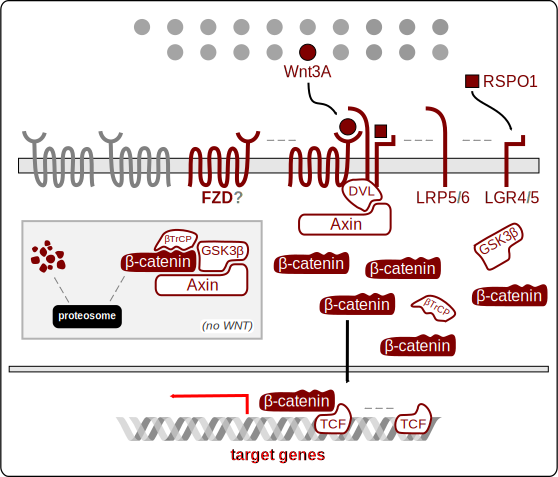
\includegraphics[width=4in]{FIGS/pathways/wnt.pdf}
  {\singlespacing 
  \caption[Structure of the canonical Wnt signaling pathway]
          {A simplified structure of the canonical Wnt signaling pathway.
          Of 19 ligands (circles), Wnt3A is the prototypical canonical ligand
          (filled red circle).
          Wnts binds to a subset of 10 FZDs, with a generally unknown degree
          of specificity. In the absence of
          Wnt (inset gray box), \bcat\ is proteosomally degraded after
          \pn\ and \ubn\ by the destruction
          complex. This complex includes the kinase \gsk, the E3 ubiquitin ligase
          \textbeta{TrCP}, and the scaffold Axin.
          In response to ligand, the destruction complex
          is disrupted in a Dishevelled (DVL)-dependent manner,
          allowing \bcat\ levels to accumulate.
          Nuclear \bcat\ binds to the co-factor TCF/Lef and together
          these factors modulate the transcriptional network of the cell.
  }
  \label{fig:pathways:wnt}}
  \end{figure}

  
  
  
  
  
\subsection{The Wnt ligands}
\label{pathways:wnt:wnt}


 \begin{figure}[!bt]
  \centering
  \includegraphics[width=4in]{FIGS/pathways/wnt_tree.pdf}
  {\singlespacing 
  \caption[Wnt pathway phylogenetic trees]
    { Phylogeny of the Wnt
      ligands (\textbf{a}, \autoref{pathways:wnt:wnt}),
      receptors (\textbf{b}, \autoref{pathways:wnt:frizzled}), and
      transcription factors (\textbf{c}, \autoref{pathways:wnt:bcat}).
      The \textit{T.a.} prefix indicates putative \ta\ proteins (gray).
      WG (Wingless), FZ (Frizzled), and ARM (Armadillo) are \fly\ orthologs
      of mammalian Wnt1, FZDs, and \bcat.
      JUP, Junctional Plakoglobin (also known as \textgamma-catenin)
      is a paralog of \bcat.
	  CTNNB1, gene symbol for \bcat.
      4F0A.B/A, identifiers for crystal structures of \frog\ Wnt8A
      and FZD8 used in the alignments. Wnt3A and Wnt5A (reds) are the
      prototypical canonical and non-canonical Wnt ligands, respectively. 
      As with the \tgfbsf\ pathway, note the high degree of diversity
      for each node when considering the basal \glspl{ta} proteins, and
      that the Wnts and FZDs each fall into multiple distinct subfamilies.
      Distances are approximate, in arbitrary length units
      (see \nameref{pathways:methods}).}
  \label{fig:wnt:trees}}
  \end{figure}



The mammalian Wnt ligands were initially identified with the discovery
of mouse Int-1, which was later found to be homologous to the \fly\
protein Wingless (WG). Mice are, of course,
wingless by default, and so in mammals these two gene names
were concatenated into the meaningless ``Wnt1.'' All other Wnt ligands
are named similarly \cite{Mikels2006}. In mammals, there are a total of
19 Wnts that fall into
multiple subfamilies by sequence homology (\autoref{fig:wnt:trees})
\cite{Clevers2006,Malhotra2009}. 


These small ligands ($\sim$350 amino acids) are highly cysteine-rich,
with 22 cysteine residues that have
conserved spacing across all Wnts. The evolutionary maintenance of these cysteines
was taken to imply the formation of intramolecular cysteine bridges, which suggested
that Wnt ligands should be stable proteins \cite{Mason1992}.
Further, aspects of the primary sequence, including many
charged residues, were suggestive of a protein that should be highly soluble.
Despite the expected stability and solubility of the Wnt ligands, they proved
to be quite problematic to work with \cite{Verheyen2010}.


In overexpression systems, intracellular Wnts were found to have many glycosylated forms and
tended to associate with chaperones, implying some difficulty in properly folding 
these proteins. Extracellular Wnts, in contrast, were found to have fewer glycosylated forms.
Further, the bulk of overexpressed Wnt products tended to remain in the cell \cite{Mikels2006},
and the Wnt proteins that left the cell tended to stay associated with membranes or with the
extracellular matrix \cite{Reichsman1996}. All of this data suggested that the Wnt
ligands were in fact neither stable nor soluble, explaining in part
the difficulty in purifying these proteins.


With the first successful purification of a functional Wnt in
2003, the explanation for the lack of solubility became clear: Wnts have an absolutely
conserved palmitoylated cysteine at the N-terminus. This lipidation is essential, as
mutant proteins lacking the lipidated cysteine
are incapable of signaling \cite{Willert2003}.
The relative insolubility of Wnt ligands have made them quite difficult to purify.
Indeed, purified Wnts are commercially available primarily through a single vendor
(R\&D Biosystems), and at
relatively low purity. As I show later in \autoref{insulation:system}
(\ar{fig:insulation:contamination}), this
low purity of the common reagent has important consequences to interpretation of
some experimental results.


To reduce experimental costs, studies therefore
frequently use Wnt-conditioned media instead of purified Wnts.
This approach suffers in that conditioned media contains a large amount of
unknown secreted cellular products. Cell lines that lack the Wnt
overexpression are often used as negative controls. However, given the degree of
transcriptional remodeling that the Wnt pathway can cause, there are likely
many unknown differences between Wnt-conditioned and control-conditioned
media.


The solubility problem for the Wnt ligands led to an additional difficulty,
that of determination of the tertiary structure of these proteins. Indeed, the first 
crystal structure of a Wnt was obtained only recently \cite{Janda2012}. The
primary sequence of Wnts are not related to any known protein fold, so prior
to the crystal structure there were many unknowns regarding how Wnts bind
to their various receptors and co-receptors. I touch on this more below.


    \begin{table}[!bt]
    \centering
	\footnotesize
    \caption[List of Wnt ligands]
            { Sequence sources for the 
              Wnt alignments in \autoref{fig:wnt:trees}. }
    \label{table:pathways:methods:wnt}
    \begin{tabular}{llll}
    \hline
    Symbol    & Species & NCBI GI & Accession \\ \hline
	Wnt1   & \textit{H. sapiens} & 4885655   & NP\_005421.1    \\
	Wnt2   & \textit{H. sapiens} & 4507927   & NP\_003382.1    \\
	Wnt2B  & \textit{H. sapiens} & 630044901 & NP\_001278809.1 \\
	Wnt3   & \textit{H. sapiens} & 13540477  & NP\_110380.1    \\
	Wnt3A  & \textit{H. sapiens} & 14916475  & NP\_149122.1    \\
	Wnt4   & \textit{H. sapiens} & 17402922  & NP\_110388.2    \\
	Wnt5A  & \textit{H. sapiens} & 371502087 & NP\_001243034.1 \\
	Wnt5B  & \textit{H. sapiens} & 17402919  & NP\_110402.2    \\
	Wnt6   & \textit{H. sapiens} & 16507239  & NP\_006513.1    \\
	Wnt7A  & \textit{H. sapiens} & 17505191  & NP\_004616.2    \\
	Wnt7B  & \textit{H. sapiens} & 17505193  & NP\_478679.1    \\
	Wnt8A  & \textit{H. sapiens} & 17505195  & NP\_490645.1    \\
	Wnt8B  & \textit{H. sapiens} & 110735437 & NP\_003384.2    \\
	Wnt9A  & \textit{H. sapiens} & 15082261  & NP\_003386.1    \\
	Wnt9B  & \textit{H. sapiens} & 17017976  & NP\_003387.1    \\
	Wnt10A & \textit{H. sapiens} & 16936520  & NP\_079492.2    \\
	Wnt10B & \textit{H. sapiens} & 16936522  & NP\_003385.2    \\
	Wnt11  & \textit{H. sapiens} & 17017974  & NP\_004617.2    \\
	Wnt16  & \textit{H. sapiens} & 17402914  & NP\_057171.2    \\
	WG     & \textit{D. melanogaster} & 17648113  & NP\_523502.1   \\
	T.a.30370& \textit{T. adhaerens}  & 196012489 & XP\_002116107.1 \\
	T.a.52489& \textit{T. adhaerens}  & 195996709 & XP\_002108223.1 \\ 
    \hline
    \end{tabular}
    \end{table}


	
	
	
	
	
	
\subsection{The Frizzled receptors}
\label{pathways:wnt:frizzled}



There are 10 human Wnt receptors, the Frizzleds (FZDs).
These are a diverse group of seven-pass G-coupled
protein receptors (GPCRs), though canonical signaling is mediated
primarily by non-G-protein mechanisms \cite{Angers2009}.
Upon binding to Wnt and various cofactors
the Wnt/FZD complex is likely endocytosed and
sequestered into multivesicular bodies within the cell. This receptor
internalization is essential to proper signaling
\cite{MacDonald2009,Taelman2010}. As a consequence of Wnt binding
to the Frizzled receptors, the transcription factor \bcat\
is stabilized. However, to date there are many competing
models and no clear front-runner for how FZD causes this outcome
(see \autoref{pathways:wnt:bcat}).


Essential for Wnt signaling through FZDs are the single-pass
transmembrane co-receptors, LRP5 and LRP6 (tongue-twistingly
expanding to ``Low-density lipoprotein receptor-related protein'' 5 and 6)
\cite{Clevers2006}. The ectodomain structure of LRP6 was recently
solved, revealing four tandem
beta-propellar-EGF-like domains that provide a large interface
for interacting proteins. Prior mutational studies of these domains
showed that they are essential for Wnt binding. Further, Dickkopf-1
(DKK1), a classical extracellular Wnt antagonist, was shown to bind
to these same domains, which would likely occlude the Wnt binding interface
\cite{Chen2011,Ahn2011,Cheng2011}. (I use purified DKK1 in
\ar{insulation:system} to demonstrate specificity of Wnt responses.)


Additional co-factors that are not essential but that dramatically
amplify Wnt signaling are the soluble protein R-spondin 1 (RSPO1)
\cite{Kim2005} and 
another subfamily of GPCRs, LGR4 and LGR5
(short for ``Leucine-rich repeat-containing G-protein coupled receptor
4 and 5''). It was recently discovered that these two co-factors
are themselves likely a ligand-receptor pair
\cite{Kim2005,Glinka2011,DeLau2011}, though the mechanism by which these co-factors
enhance Wnt signaling is still a mystery.


With ten receptors and multiple co-factors, we are left with the issue of
signaling specificity.
Wnts appear to have high promiscuity for the \fz s, with little
certainty in the field regarding which, if any, receptor-ligand pairings are excluded.
It is still unknown which Wnts bind to
which \fz s, or if \fz s can generally signal in both canonical and non-canonical ways
\cite{Angers2009,VanAmerongen2012}.
Unfortunately, while Wnt3A and Wnt5A are generally
considered to be the prototypical ligands for canonical and non-canonical
Wnt signaling, respectively  \cite{Huang2004}, there is
evidence that each can transduce signals through a non-prototypical pathway
under certain conditions \cite{VanAmerongen2012}.
The recent crystal structure of \frog\ Wnt8 with FZD8
did little to enhance our
understanding of the origins of receptor-ligand specificity,
as the intra-protein contacts occurred primarily at highly conserved
Wnt residues \cite{Janda2012}. This is suggestive that there is either
little specificity between ligands and receptors, or that specificity
is a more complicated outcome of interactions with other factors.




    \begin{table}[!bt]
    \centering
	\footnotesize
    \caption[List of Frizzleds]{ Sequence sources for the 
    Frizzled (FZD) alignments in \autoref{fig:wnt:trees}. }
    \label{table:pathways:methods:frizzled}
    \begin{tabular}{llll}
    \hline
    Symbol & Species & NCBI GI & Accession \\ \hline
	FZD1  & \textit{H. sapiens} & 4503825   & NP\_003496.1    \\ 
	FZD2  & \textit{H. sapiens} & 4503827   & NP\_001457.1    \\ 
	FZD3  & \textit{H. sapiens} & 8393378   & NP\_059108.1    \\ 
	FZD4  & \textit{H. sapiens} & 22547161  & NP\_036325.2    \\ 
	FZD5  & \textit{H. sapiens} & 27894385  & NP\_003459.2    \\ 
	FZD6  & \textit{H. sapiens} & 257470999 & NP\_001158087.1 \\ 
	FZD7  & \textit{H. sapiens} & 4503833   & NP\_003498.1    \\ 
	FZD8  & \textit{H. sapiens} & 13994190  & NP\_114072.1    \\ 
	FZD9  & \textit{H. sapiens} & 4503835   & NP\_003499.1    \\ 
	FZD10 & \textit{H. sapiens} & 6005762   & NP\_009128.1    \\ 
	FZ    & \textit{D. melanogaster}  & 17864440  & NP\_524812.1 \\
	T.a.12196 & \textit{T. adhaerens} & 196002269 & XP\_002111002.1 \\
	T.a.31674 & \textit{T. adhaerens} & 196014261 & XP\_002116990.1 \\
    \hline
    \end{tabular}
    \end{table}

	

\subsection{\bcat, the canonical Wnt effector}
\label{pathways:wnt:bcat}


\bcat\ is the main effector of canonical Wnt signaling. This
large protein is one of several catenins that are
used in cellular adhesion. \bcat\ itself has a large
membrane-associated pool dedicated to this task \cite{Jamieson2012}, while only a
``vanishingly small'' baseline cytosolic component is found
in Wnt un-stimulated cells \cite{Li2012}.


In the classic model of Wnt signaling, basal
\bcat\ is constitutively transcribed and translated, but then degraded
just as quickly in the absence of Wnt. Wnt stimulation stabilizes
\bcat, thus allowing cytosolic levels to build. In some systems,
cytosolic \bcat\ accumulation is measureable in as little as 15 minutes,
and reaches a stable peak response by 2 hours that can last longer
than 24 hours \cite{Li2012,Hernandez2012}.
The nuclear import/export rates for \bcat\ are unaffected by signaling,
and so it appears that nuclear accumulation resulting from Wnt 
signaling is due to an
overall change in protein abundance throughout the entire cell 
\cite{MacDonald2009,Clevers2006}.


Importantly, \bcat\ appears to encode information about extracellular
Wnt concentrations primarily in its nuclear concentration, as opposed to the
concentration of particular phosphorylation states. While various \bcat\ 
phospho-states have been discovered and claimed to
be required for the transcriptional activity of this protein, careful
quantification of post-signaling protein levels revealed that the vast
majority of \bcat\ is not phosphorylated in the presence of Wnt. Instead,
the phospho-state ends up at similar concentrations to the basal state \cite{Hernandez2012},
implying that phospho-\bcat\ does not encode Wnt ligand concentrations.


It is interesting to note that, like with the \tgfbsf\ pathways, the large
number of ligands and receptors end up bottlenecking to a small number of
effectors. This bottlenecking is more dramatic in the case of Wnt, as there
is only one \bcat\ gene to which all canonical Wnt signaling leads.
There is a highly homologous paralog, \textgamma-catenin
(also called Junctional Plakoglobin, JUP),
that differs from \bcat\ to a similar degree as does the functionally identical
\fly\ ortholog, Armadillo (see \autoref{fig:wnt:trees}). \textgamma-catenin
appears to have some functional redundancy to \bcat, and even after deletion of
both catenins some Wnt signaling has still been shown \cite{Malhotra2009}.
However, it appears that \bcat\ is the primary mediator of canonical Wnt
signaling. Interestingly, similarly to the \tgfbsf\ pathways described
earlier, this severe bottleneck implies that cells cannot
know which Wnt or Frizzled activated the pathway, unless an additional channel
of signaling carries this information.


To enact its transcriptional functions, accumulated nuclear
\bcat\ partners with one of a set of transcription
factors in the TCF/Lef family (standing for T-Cell Factor/Lymphoid 
enhancer-binding factor). There are four such proteins in mammals
that appear to be functionally redundant but do have different expression
patterns \cite{Clevers2006}. These are TCF7, TCF7L1, TCF7L2, and LEF1.
TCF1 was first discovered as a factor involved
with T-cell differentiation (hence the name) \cite{VandeWetering1991}, and later
connected to Wnt signaling after finding that a \frog\ ortholog, Xtcf-3,
could cause \bcat\ nuclear translocation \cite{MOLENAAR1996}.
TCF/Lef is normally bound to the protein Groucho, which prevents association of TCF/Lef
with \bcat. This block is lifted in response to Wnt signaling after \ubn\
of Groucho by XIAP (X-linked inhibitor of apoptosis) \cite{Hanson2012}.
It has been proposed that TCF/Lef binding to \bcat\ is stable enough to
effectively sequester it in the nucleus
and so allow for long-term Wnt signaling \cite{Jamieson2012},
though to my knowledge this has not been explicitly tested.


In complex with TCF/Lef, nuclear \bcat\ is able to bind to a diverse set of
promoters and modulate transcription. These targets are highly context-dependent,
though the negative auto-regulator Axin2 is considered to be a conserved
target of \bcat\ \cite{Clevers2006,Hatzis2008}. All canonical Wnt signals
are encoded into nuclear \bcat\ concentrations, therefore ligand-
and receptor-specific information must be lost during signal transduction.
This implies that the context-dependency of Wnt signaling responses should
be the result of transcriptional idiosyncrasies or of additional information
channels (e.g. non-canonical Wnt pathways).


\subsection{The destruction complex}
\label{pathways:wnt:destruction}


The functional effect of FZD, after binding Wnt,
is to relieve the otherwise constitutive degradation of \bcat. 
The set of proteins that are involved
with \bcat\ degradation is referred to, ominously,
as the ``destruction complex.'' The mechanisms by which this
complex degrades \bcat\ are fairly well understood, but how
active FZD causes an end to the destruction is still
highly contentious \cite{Hernandez2012,Li2012}.
Here, I discuss the components of this
complex that are best understood, and that will become important
later in the discussion on crosstalk between Wnt and \tgfbsf\
(\ar{pathways:wntTgfb:mechanism}).


\subsubsection{\gsk}

The protein Glycogen synthase kinase 3 beta (\gsk) maintains
a central role in the destruction complex. In fact, \gsk\ is
a signaling hub for many pathways, making it a prime node
for signal integration. \gsk\ is inhibited by Insulin and
growth factor signaling, which lead to phosphorylation of its N-terminal
tail. The phosphorylated tail becomes a ``pseudo-substrate'' that competes with the
actual substrates of \gsk. However, while this mechanism of inhibition
is well established, it is not clear if it is used by the Wnt
pathway. Nor is it clear whether the Wnt pathway maintains
a distinct pool of \gsk\ from growth factor pathways that can act
as an insulated information channel. If not, then modulation of a
common pool of \gsk\ by Wnt or other pathways would necessarily
create inter-pathway crosstalk.


What is clear is that this kinase requires ``priming'' phosphorylation
by another member of the \bcat\ destruction complex,
Casein Kinase 1 alpha (CK1\textalpha). This priming stems from phosphorylation 
of \bcat\ by CK1\textalpha, which produces a recognition site for subsequent
phosphorylation of \bcat\ by \gsk. Phosphorylation by
\gsk\ in turn creates a recognition site for the the ubiquitin E3 ligase
BTRC (beta-transducin repeat-containing protein, also known as \textbeta{TrCP}),
which subsequently ubiquitinates \bcat\ and sends it
off to the grinding mill of the proteosome
\cite{Frame2001,Hernandez2012}. The widely described model of
Wnt signaling has this \gsk-mediated phosphorylation being somehow
prevented in the presence of Wnt, though exactly how is a major subject of debate.
In any case, pharmacological inhibition of \gsk\ by LiCl
\cite{Stambolic1996,Hedgepeth1997} or the
ATP analog BIO \cite{Meijer2003} is sufficient to induce large increases in \bcat\ levels.
Inhibition of \gsk\ is therefore commonly used to experimentally simulate Wnt
treatment, as it gets around the earlier-mentioned difficulties
of working with purified Wnt ligands. Care should be taken when interpreting
results of these experiments, as disentangling \gsk/\bcat\ effects from the myriad of other
\gsk-mediated effects is non-trivial.


\subsubsection{Axin and APC}

There are two large proteins that act as scaffolds on which the drama
of \bcat\ destruction unfolds. These are Adenomatous
Polyposis Coli (APC) and Axin. Despite general agreement that APC is involved
in this process, its effects are often incongruous between experiments
and systems, and so there is a lack of consensus
for what APC actually does in the complex \cite{Li2012}. The roles
of Axin are better understood, and it is generally believed that
this protein forms the primary scaffold of the \bcat\ degradation
complex \cite{Roberts2012}.


Until recently, a prevailing model was that APC, which is known to
be a mobile protein, would drag the destruction complex to an unknown
subcellular compartment in order for \bcat\ degradation to occur.
However, a careful study found that APC could
effectively block Wnt signaling no matter its localization. This was
done by expressing APC constructs, modified with various localization
signals to specific compartments, in the background of APC-null cell types
\cite{Roberts2012}. All variants allowed continued \bcat\ destruction,
which convincingly disproves the APC localization model.


There exists some structural work showing the binding of APC and Axin
to one another. Intriguingly, these studies reveal that Axin binds using
a region with homology to Regulator of G-Protein Signaling (RGS)
sequences \cite{Spink2000}. Because FZDs are GPCRs (and GPCRs activate G-proteins), it is
intriguing that Axin has an RGS domain, though to my knowledge no
functional link has been demonstrated. More important is the fact that
Axin and APC appear to bind to the same interface of \bcat\ \cite{MacDonald2009},
implying that they should compete for \bcat\ binding. This is especially
important because Axin levels are widely-cited to be extremely low in cells \cite{Lee2003},
such that even a small change in its concentration (e.g. via overexpression)
would then affect the balance of APC versus Axin binding to \bcat.


\subsubsection{Dishevelled}


Immediately downstream of FZD, before the destruction complex,
is the protein Dishevelled (DVL), named
for the phenotype of the \fly\ ortholog. This component is absolutely required for
Wnt signaling in general, including non-canonical, though its precise
role is something of a mystery \cite{Angers2009,Gao2010}.
There are three paralogs in mammals, though they have a high degree
of functional redundancy and so likely differ primarily in expression pattern
(DVL1 or DVL2-null mice are viable, though
DVL3-null mice die of developmental heart defects \cite{Gao2010}).


\subsubsection{Mechanisms of destruction}


Having completed a brief tour of the destruction complex components,
I turn to the mechanisms by which Wnt signaling modulates activity of the complex.
The favored models of Wnt-induced \bcat\ stabilization involve
disabling the destruction complex so that \bcat\ phosphorylation,
and subsequent degradation, is reduced. How it does so is still contentious;
I review a few competing models below.


DVL has
a structural PDZ domain that binds to \fz, and DVL and Axin both contain
DIX domains. The homologous DIX domains of these two proteins have been proposed to
allow them to polymerize,
yielding a model wherein FZD activation pulls Axin to the membrane,
through a DVL bridge, thus disrupting the destruction complex \cite{MacDonald2009,Gao2010}.
No definitive evidence for this model has been
established, though the components can be found together in internalized endosomes during
Wnt signaling events. This suggests sequestration as a possible mechanism
for DVL-mediated Wnt signaling \cite{Angers2009}. LRP6, a Wnt co-receptor,
has been similarly proposed
to pull Axin to the membrane. This is consistent with overexpression of either DVL or an LRP6
endodomain fragment being sufficient to induce
increased \bcat\ levels \cite{MacDonald2009,Taelman2010}. This is the model
that I show in \ar{fig:pathways:wnt}.


Sequestration of the Wnt signaling complex into internal
compartments, causing isolation from interactions with cytosolic proteins
like \bcat, is a mechanism with strong support \cite{Taelman2010}.
However, there are some inconsistencies with this model. The primary
mediators of the destruction complex, Axin and \gsk, are
constitutively expressed, such that they would have to be
continuously sequestered to prevent new protein products from slowly
causing a decay in \bcat. Axin is eventually destabilized by Wnt
signaling, which gets around this caveat, but while this occurs
Axin2 levels are increased to compensate. Therefore the long-term
maintenance of Wnt activity becomes hard to explain \cite{Hernandez2012}.


Further, the key study showing this receptor-Axin complex
sequestration also found that global protein levels increased in
cells after Wnt treatment, which they interpreted to be due to
removal of a significant enough fraction of \gsk\ to also decrease its
suppression of non-Wnt proteins \cite{Taelman2010}. Given the
extremely low quantities of Axin in cells \cite{Lee2003}, and the fact
that its interaction with the much more abundant \gsk\ is stoichiometric,
it not clear how a Wnt signal could so significantly impact global
\gsk\ signaling by sequestration of the destruction complex-associated pool.
Recent work is suggestive that the global increase in protein levels
after after a Wnt response is instead due to a cell-cycle dependent
form of non-canonical signaling \cite{Acebron2014}.


In addition to the sequestration model, active
FZD complexes could negatively affect \gsk, Axin, the priming kinase CK1\textalpha,
or some combination of these. All models have support, though
the experimental bases for these models nearly universally
depend on overexpression or knockdown of pathway components \cite{Hernandez2012,Li2012}. While use of such dramatic pathway modulation
does not negate the results, it does complicate the interpretation of those results. Recent work
has begun to make use of endogenous protein levels, which has led to two strong
but incompatible models.


In the first model, the authors take an Axin-centric focus,
making the assumption that all Wnt-relevant \bcat\ destruction is mediated by
Axin \cite{Li2012}. They therefore rely on
co-immunoprecip-itation (co-IP) of endogenous Axin
for all experiments. Using this approach, they show that endogenous Axin
levels remain mostly unchanged during the early Wnt response, implying that modulation
of Axin levels is not the primary mechanism of \bcat\ stabilization
(though this does not rule out
non-degradative forms of modulation).
Instead, the authors were surprised to find that Axin pulled down minimal
\bcat\ in the absence of Wnt, and that Wnt signaling caused more \bcat\
to associate with Axin. They interpreted this to mean that interactions
on this scaffold are normally transient, but that Wnt signaling blocks
some step and so renders the destruction complex inert by saturating it
with non-transient \bcat\ binding. 
With the additional finding that Axin-bound \textbeta{TrCP}
dropped rapidly after Wnt treatment, the authors concluded that Wnt
activity somehow blocks \ubn\ of \bcat\ instead of phosphorylation.


In opposition to the saturation model, another careful study
used kinetic arguments and careful measurements of protein
quantities to show that it is indeed the \pn\ steps that control the Wnt
response \cite{Hernandez2012}. The authors start from the position that
the current models, including the saturation model, are insufficient to
explain the kinetics of the \bcat\ response to Wnt. In particular, the
models fail to explain the maintained high level of \bcat\
after $\sim$2 hours.
They show experimentally that the destruction complex is functional
whether or not Wnt is present, which directly argues against the saturation
model. Further, the authors show mathematically that a saturation-based mechanism
would have a limited range for regulation. Finally, their kinetic models
demonstrated that all observed dynamics of the pathway response could be explained
by the degree of \pn\ at two sites within \bcat. As I note in
\ar{introduction:hierarchy}, however, agreement with an abstract model
does not imply that the model is correct.


What can we make of this general confusion in the field for how Wnt
causes an increase in its effector, \bcat? First, recent studies that
focus on endogeous protein levels are clearly moving in the right
direction, and I think that the contradictions between the current
best studies will begin to be resolved by future use of similarly clean, endogenous approaches.
For my own work, I decided that it was best to avoid favoring one
model over another, since defining experiments with respect to such
tenuous models would make the future of their interpretation
uncertain. For this reason, I take a simple, mechanism-independent approach
to Wnt signaling that only requires that extracellular Wnt concentrations
are encoded as intracellular \bcat\ concentrations (\ar{insulation:introduction}).


    \begin{table}[!bt]
    \centering
	\footnotesize
    \caption[List of catenins.]{ Sequence sources for the 
    Wnt-related catenin alignments in \autoref{fig:wnt:trees}. }
    \label{table:pathways:methods:bcat}
    \begin{tabular}{lllll}
    \hline
    Symbol    & Name               & Species & NCBI GI & Accession \\ \hline
	CTNNB1    & \bcat\             & \textit{H. sapiens}      & 148233338 & NP\_001091679.1 \\
	JUP       & \textgamma-catenin & \textit{H. sapiens}      & 4504811   & NP\_002221.1    \\
	ARM       & Armadillo          & \textit{D. melanogaster} & 24639204  & NP\_476665.2    \\
	T.a.22780 &                    & \textit{T. adhaerens}    & 196000871 & XP\_002110303.1 \\
    \hline
    \end{tabular}
    \end{table}

    

    
\subsection{Non-canonical Wnt signaling}
\label{pathways:wnt:noncanon}


Our understanding of the
best-understood Wnt signaling pathway, the canonical pathway, is still
incomplete. The various non-canonical Wnt signaling
pathways are even less understood. This in large part because the readouts
of these pathways
are either hard to measure or are affected by other factors whose contributions are
difficult to disentangle \cite{Angers2009,VanAmerongen2012}.
Though the focus of this dissertation is on canonical signaling, here I briefly
review the non-canonical pathways to provide background for
an instance of inter-pathway crossalk between \tgfbsf\
and non-canonical Wnt5A signaling.


There are many different non-canonical pathways, with some authors counting
up to ten \cite{Malhotra2009}, though the true number is
certainly unknown. Perhaps the best-studied non-canonical
pathways are those of Planar Cell Polarity (PCP) and Convergent Extension (CE) in \fly.
However, it is important to note that these pathways are studied in different
systems (the wing and developing embryos, respectively)
and share core components, so it is unclear how distinct these pathways truly
are \cite{VanAmerongen2012}. This ambiguity is common among the non-canonical pathways. An additional
non-canonical pathway studied in mammalian systems activates
Ca$^{2+}$ signaling, though the consequences of such
signaling are mostly unknown \cite{De2011}.


While the mechanisms, readouts, and functional consequences of non-canonical signaling
are poorly understood, there are several key components that are well-established.
At the level of receptors, ROR2 (expanding to ``Receptor tyrosine kinase-like
orphan receptor'') has an extracellular Wnt-binding domain homologous to
that of FZD. This receptor activates Ca$^{2+}$ signaling in response
to Wnt5A. The ROR2 homolog ROR1 also has this domain,
but may be a pseudo-kinase \cite{VanAmerongen2012}.
Importantly, Wnt5A signaling through ROR2 is well established to inhibit long-term
canonical Wnt/\bcat\ signaling, though how it does so is still unknown
\cite{Huang2004,Angers2009,Malhotra2009,VanAmerongen2012}.


Downstream of the receptors, DVL is frequently (but not always) 
required for non-canonical signaling. Interestingly, DVL seems to use different
protein domains for canonical and non-canonical signaling, so that mutation of
one domain can preferentially block one type of signaling \cite{Gao2010,VanAmerongen2012}.


Finally, there is no good reason to believe that canonical and
non-canonical signaling must occur in isolation. Because of the
promiscuity of Wnt-FZD binding and the unknown contribution of each
FZD to the various Wnt signaling pathways, it is reasonable to
expect that a Wnt signal may trigger multiple simultaneous downstream pathways.
Perhaps this is a mechanism by which the cell obtains more information
about the original signal, since \bcat\ concentrations alone can only encode
information about the overall extent of canonical Wnt activity, not which 
Wnts triggered that activity.

\section{Functional importance of \tgfbsf\ and Wnt signal integration}
\label{pathways:wntTgfb:function}


Having covered the canonical \tgfbsf\ and Wnt signaling pathways, we
can now move forward to the topic of this dissertation: inter-pathway crosstalk.
The goal of this section is to both motivate the study of Wnt/\tgfbsf\
crosstalk and to review the work that has been done in this field.
There are many systems in which both of these pathways are intensively
studied (indeed entire
textbooks have been written on these pathways). However, most of this work
studies each pathway indepenently; there exists a much
smaller body of work on Wnt/\tgfbsf\ inter-pathway
crosstalk. One of the more experimentally-tractable of such systems is the
adult mammalian gut, and so I focus my review on this system.


The study of adult stem cells has advanced rapidly in recent years,
especially with the identification of resident stem cells for several
tissues \cite{Barker2010} and with the discovery that differentiated
cells can be turned pluripotent by expression of a handful of
transcription factors \cite{Takahashi2006}.
However, there is still much that we do not understand about stem
cell biology in general, especially because \i{in vitro} studies
are difficult to map back to \i{in vivo} phenomena,
and because each stem cell system has proven to have its own quirks including
differential use the same genetic pathways.


In particular, work in this field has
pointed toward \tgfbsf\ signaling being a major factor in stem cell
differentiation, while canonical Wnt signaling seems to control stem cell
maintenance. There are cases where this oppositional role assignment does not occur
\cite{VonBubnoff2001,Fischer2002,Nakashima2005,Itasaki2010a,
Feigenson2011,Lander2012,Malhotra2009,Davidson2012}, though
it is fairly common across stem cell systems
\cite{Verheyen2010,Libusova2010,Gregorieff2005,VandeWetering2002,
Schepers2012,Teo2006}. These roles are
particularly well-studied in the context of the mammalian intestine.


Our understanding
of the intestinal stem cell system has increased significantly in recent years,
due in no small part to the work of Hans Clevers and colleagues.
Clevers' group has dissected the function of many genes involved with
intestinal stem cell development (with a focus on canonical Wnt), has
unambiguously identified the stem-cell population \cite{Barker2007a},
and has developed an \textit{in vitro} system for culturing intestinal
stem cells in such a way that they behave like homoestatic \textit{in vivo} crypts
\cite{Sato2011a,Sato2011b}. This work has even led to successful engraftment
of intestinal stem cells isolated from one mouse into the damaged
intestine of another \cite{Yui2012}. Given the potential value to stem
cell therapy, and the connection of stem cells with colon cancer
\cite{Zeki2007,Barker2009a}, a deeper understanding of intestinal stem
cells is highly sought after in hopes of obtaining new therapeutic strategies
for many bowel diseases.


While the gut stem cell system is highly studied, it is poorly understood
how intestinal stem cells
integrate distinct signals from their environment, such as Wnt and \tgfbsf,
and thus choose one of several differentiated outcomes. Given the oppositional
roles of \tgfbsf\ and Wnt in the gut, and their various functional interactions in other systems
\cite{Attisano2004,Labbe2007,Chong2009,Itasaki2010a,Minoo2010a,
Serra2011,Feigenson2011,Rodriguez-Carballo2011,Chen2012a,Akhmetshina2012,Song2014},
it is important to understand generally how cells integrate these two signals.


\subsection{\tgfbsf\ and Wnt in the intestinal crypt}
\label{pathways:wntTgfb:gut}

\subsubsection{Crypts are the functional unit of intestinal epithelium}

The small and large intestine both contain
similar stem cell systems. Between these two organs, morphological
differences in stem cell systems are revealing in terms of the distinct organ functions.
The small intestine contains a high fraction of absorptive cells (enterocytes)
and an increased epithelial surface area due to relatively large lumenal projections termed
villi, consistent with its role in digestion and absorption of food.
The colon is predominantly made up of mucus-secreting goblet cells
and completely lacks villi, consistent with its need to carry potentially
abrasive and toxic waste \cite{Iacopetta2002}. The protective role of
goblet cells is highlighted by the connection between goblet cell
loss and rapid tumor formation in mice \cite{Yang2008}. The colon is of
particular clinical interest due to the high rates of cancer
and inflammatory diseases of this organ \cite{Jemal2010}. Despite macroscopic differences
in morphology, many aspects of of the stem cell biology seem to be similar
in the small and large intestine.


A cross-section of the intestine would reveal a hollow tube whose wall
consists of several tissue layers. The
most-lumenal layer consists of the mucosa, a single sheet of epithelium
over stromal tissue (fibroblasts, collagen, blood/lymphatic vessels, etc.),
together forming crypts and their support structures.
The epithelium sits atop a basement membrane
\cite{Simon-Assmann2010} which in turn is immediately adjacent to
myofibroblasts such that each crypt is essentially sheathed in these cells.
Though it is likely that important signaling takes place between the
epithelium and stroma \cite{Simon-Assmann2010,Kosinski2010,Ingham2011},
these signals are difficult to study and their importance is unclear given
the fact that \i{ex vivo} isolated crypts maintain a differentiating,
homeostatic structure even in the
absence of a macroscopically polarized stroma \cite{Sato2011a,Lahar2011}.


The crypts are the functional unit of the intestine. The single epithelial layer
of each crypt contains only
$\sim$10 stem cells at the base that divide on average once per day,
generating a conveyor belt of rapidly dividing and differentiating cells
\cite{Snippert2010} \arp{fig:pathways:crypt}. These ``transit amplifying'' cells stop dividing
after full differentiation and are eventually lost to the lumen of the gut
\cite{Eisenhoffer2012}. This process is fast, such that the entire non-stem
cell population of a crypt is turned over every 3-5 days \cite{Buske2011}.


In the small intestine, the top of the crypt (which is the base of
the villus) is roughly the point at which cells are completely differentiated.
Note that this generally accepted model of crypt turnover
is based on studies of the small intestine and is thought to be similar in
the colon, though there are important
differences between the organs that should be considered.
For example, the large intestine completely lacks the paneth cells that have
recently been reported to be required for stem cell maintenance in the small
bowel. However, colonic crypts do contain cells
expressing similar surface proteins \cite{Sato2011b}.
Additionally, the entirety of the colonic crypt contains apparently-differentiated
cells, suggesting that the transit amplifying population
is much smaller than in the small bowel.
On the other hand, the literature generally supports that the population
dynamics and signaling factors are similar between the small and large
intestine, and between mouse and human.


	\begin{figure}%[ht]
	\centering
	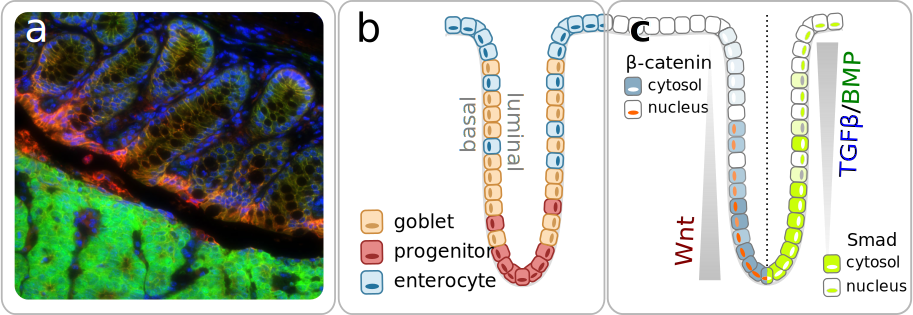
\includegraphics[width=6in]{FIGS/pathways/crypt.pdf}
	{\singlespacing 
	\caption[Expression patterns of Wnt and \tgfbsf\ in colonic crypts]
            { Overview of \tgfbsf\ and Wnt signaling patterns
            in the colonic crypt. \b{a}, Immunostained crypts
            from a CPC;APC mouse \cite{Hinoi2007} showing two opposing sides pinched
            together, with the dark lumen in between. Blue, DNA; green,
            \bcat, red, E-cadherin. The bottom set of crypts are tumorous;
            note the global increase in \bcat. Image curtesy Michael
            Ramirez and Curtis Thorne (Altschuler \& Wu lab,
            Univeristy of Texas Southwestern).
            \b{b}, Cartoon of colonic crypt
            structure, showing key cell types. \b{c}, Cartoon of
            signaling gradients in the crypt, showing high Wnt
            at the crypt base and high \tgfbsf\ at the crypt tops.}
	\label{fig:pathways:crypt}}
	\end{figure}



\subsubsection{Opposing gradients of \tgfbsf\ and Wnt in crypts}


Within the crypt epithelium, there are distinct patterns of expression for
the Wnts and the \tgfbsf\ ligands that together seem to control cell
fate in a crypt-axis positional manner. Using fluorescence in situ hybridization
(FISH), Clevers' group showed that canonical Wnts and various FZDs were
preferentially expressed in the crypt base, while non-canonical Wnts were
expressed throughout the crypt or only at the top \cite{Gregorieff2005}.
The same group later found that LGR5, a Wnt co-receptor,
is a highly specific marker for intestinal stem cells \cite{Barker2007a}.
This discovery allowed for labeling and purification of this cellular population,
and the demonstration that this cell type alone could
re-create crypt-like structure \i{in vitro}.


There is evidence that the paneth cell population is the source
of canonical Wnt3A in the crypt base \cite{Sato2011b},
though this is confounded by a study showing that this cell
type can be ablated \textit{in vivo} without loss of stem cell maintentance
\cite{Rizk2012}.
In contrast to canonical Wnt, but similarly to non-canonical Wnt,
\tgfbsf\ ligands and receptors are expressed exclusively in the
the differentiated epithelium at the tops of the crypts
\cite{Hardwick2004,Massague1990}
and villi \cite{Yamada2013}. Smad activity is restricted to
the same parts of the crypt \cite{Hardwick2008,Libusova2010}.


How the gradients are established and maintained, especially in the face
of a constanty turning over cell population, is not well understood.
The relatively long lifespans of the paneth cell population
\cite{DeSantaBarbara2003} hint that this
cell type may serve as a sort of anchor for these gradients. Another
potential source of gradient maintenance are the transmembrane ephrin
receptors and their ligands, which seem to be required for proper cell sorting: their
loss results in disorganized cellular positions within colonic crypts.
Intriguingly, these ephrins and receptors are regulated by canonical Wnt signaling,
though how these two phenomena interact is unclear \cite{Batlle2002}.


Importantly, it is unclear whether these gradients actually function as such.
While the gradients could be formed by secreted molecules diffusing over
multiple cell lengths, the relative insolubility of Wnts argues against this.
Indeed, in the developing fly wing and in the vertebrate notochord, there is
recent evidence that diffusion of Wnt is not the mechanism by which it creates
gradients \cite{Alexandre2014,Serralbo2014}. Additionally, because Wnt and \tgfbsf\
have so many extracellular antagonists, the presence of a ligand gradient is neither
required nor sufficient to have a functional gradient \cite{Wakefield2013}.


\subsection{Wnt drives stem cell maintenance; \tgfbsf\ drives differentiation}

While the opposing gradients of these two pathways hint at
opposing functional roles, they do not imply it. 
The gradients could be a macroscopic consequence of cell sorting.
Or, the gradients could be a marker of crypt position without exerting any
concentration-dependent influence.
The biological argument that most favors truly oppositional roles is that
modulation of one pathway, experimentally or in the context of disease,
is generally paired with opposite deviations of the other pathway.
I reviews examples of this below.


\subsubsection{Increased Wnt signaling is a driver of colon cancer}

It is well established, and has been for some time, that over-activation of
canonical Wnt is a primary force in colon cancer. Multiple components of
the pathway have been implicated in this disease, though clearly some of
the signaling nodes are easier to hijack than others. One could imagine
upregulation of Wnts, receptors, or \bcat\ as possible
mechanisms. However, the pathway
has negative feedback, via \bcat-mediated expression of Axin2, and 
so constitutive upstream activity would be insufficient for maintenance of
high \bcat. Therefore constitutively high \bcat\
activation is more easily obtained by blocking the function of the destruction complex.
Perhaps for this reason, the most commonly modulated signaling
nodes are components of the complex itself. There is at least one example
of receptor-level modulation, however, which is that RSPO1
(the soluble Wnt co-factor) is frequently
upregulated in colon cancer due to genomic translocation \cite{Seshagiri2012}. Whether this
upregulation is functionally important to cancer, however, is still speculative.


By far, the most common Wnt pathway modification in colon cancer is mutation
of APC, the destruction complex component with perhaps the most mysterious functional role.
In fact, APC is nearly always mutated in this type of cancer ($>$80\% of cases)
\cite{He1998,Clevers2006,Roberts2012}. Interestingly, APC is rarely completely lost,
instead being frequently truncated to its
N-terminal half. The reason for this truncation preference
is unclear and has been the cause of much speculation \cite{MacDonald2009}.
However, it is worth noting that there need not be a reason.
Perhaps there are more ways to mutate APC such that it is truncated instead
of ablated, in which case truncation would simply be the more likely
evolutionary step. However, there is some cell culture evidence that APC-truncated
and APC-null cells have different phenotypes, especially with respect to cell
adhesion and migration \cite{Burgess2011}.


While it is not clear what exactly APC is doing in the destruction complex,
the effects of APC loss on Wnt signaling are well-established.
APC knockdown results in rapid nuclear accumulation of \bcat, followed by increasingly
dense cell packing due to overgrowth and then, eventually, a less-differentiated
cellular phenotype \cite{Sansom2004}. Remarkably,
stem cell-specific deletion of APC leads to adenoma formation
in mere days and results in macroscopic tumor development in only 3-5 weeks
\cite{Barker2009a}. Importantly, this effect requires
\bcat-dependent expression of Myc \cite{He1998},
a classic oncogene, as ablation of Myc can rescue the APC mutant phenotype \cite{Sansom2007}.


\subsubsection{Decreased \tgfbsf\ is a driver of crypt dysplasia} 


Given my earlier description of the \tgfbsf\ pathways as inducers of differentiation,
it is perhaps no surprise that these pathways tend to be lost in colon cancer
and in other dysplastic diseases. As with the Wnt pathway, certain components of the
\tgfbsf\ pathways are more prone to being hijacked by disease than others.
Loss of any particular \tgfbsf\ ligand would likely be insufficient to ablate pathway
activity, as would loss of several of the receptors, given the redundancy at this
level of signal transduction. The obvious targets then are the Smads, which are indeed
mutated or lost in the context of several dysplasias.


Of the Smads, the most efficient target of ablation in disease would be Smad4,
since it is the bottleneck for all upstream \tgfbsf\
pathways. Indeed, Smad4 is commonly mutated in colon cancer ($>$15\% of cases) and
in pancreatic cancer ($>$50\% of cases) \cite{Levy2005,Seshagiri2012}. Additionally, next-generation
sequencing of $>$70 human colon tumors revealed a high prevalence of Smad2 (one
of the \tgf-specific rSmads)
mutations \cite{Seshagiri2012},
allowing speculation on the importance of \tgf\ signaling in colon cancer.
In another dysplastic
disease, Juvenile Polyposis, BMP signaling loss is found in $>$50\% of cases
\cite{Haramis2004a,Miyazono2005,Hardwick2008}. Though it is unknown if the BMP loss in
these cases was sufficient
to cause the human phenotype, overexpression of the BMP-inhibitor Noggin
is sufficient to generate ectopic crypts within the villi of mouse models \cite{Haramis2004a}.


The above data suggest that gain of Wnt signaling has a more potent effect
than does loss of \tgfbsf\ signaling, at least in the context of colon cancer.
However, changes to one of these pathways is always accompanied by changes in the other.
For example, BMP signaling has been found to be reduced
in $>$70\% of colon cancers \cite{Hardwick2008}, though only $\sim$15\% of cases
have mutations in the pathway. Further, in a study of microarrays from 250
colorectal tumor samples it was found that Smad4 and
\bcat\ levels were generally anti-correlated
\cite{Freeman2012}. Taken together, these correlative
results are suggestive that these two pathways
are in some way regulating one another, and that for Wnt signaling to become
tumorigenic it has to suppress the
\tgfbsf-mediated drive towards cellular differentiation.



\section{Nodes of crosstalk between \tgfbsf\ and Wnt}
\label{pathways:wntTgfb:mechanism}


In this dissertation I am interested in understanding the inter-pathway
crosstalk between \tgfbsf\ and Wnt. As discussed in \ar{introduction:encoding},
one of the most problematic aspects of studying cell signaling
is the determination of which input signals a cell cares about
and into what intracellular property that information is encoded.
As this chapter has so far detailed, the field consensus for both
\tgfbsf\ and Wnt is that it is the concentration of the ligands
that carries the information that cells care about
(these are morphogenic signals) and this
information is encoded into nuclear concentrations of canonical
transcription factors.


Further, the literature reviewed in the previous section
strongly suggest that the \tgfbsf\ and Wnt
pathways have many opportunities for crosstalk, especially in the
mammalian gut. With established input/output relationships
in hand, and reason to suspect that the pathways in question modulate one
another, we can begin to ask how these pathways integrate information.
This section provides a review of the signaling nodes at which
inter-pathway crosstalk is thought to occur (see the graphical
summary in \ar{fig:pathways:xtalk}).




  \begin{figure}[!bt]
  \centering
  \includegraphics[width=4in]{FIGS/pathways/tgfb_wnt_xtalk.pdf}
  {\singlespacing 
  \caption[Overview of Wnt and \tgfbsf\ pathway crosstalk]
        { Overview
          of Wnt and \tgfbsf\ pathway crosstalk. 
          This dissertation focuses on canonical Wnt, BMP, and \tgf\, as mediated by Wnt3A,
          BMP4, and \tgf 1/3. Dashed lines indicate
          literature-established
          links between pathways. References:
          \textit{a}\cite{Warner2003,Warner2005a,Liu2006};
          \textit{b}\cite{Mamidi2012};
          \textit{c}\cite{Fuentealba2007,Guo2008};
          \textit{d}\cite{Furuhashi2001,Guo2008,Liu2006b};
          \textit{e}\cite{Candia1997};
          \textit{f}\cite{Zeng2008}.}
  \label{fig:pathways:xtalk}}
  \end{figure}




\subsection{Smad and DVL}
\label{pathways:wntTgfb:dvl}

The DVL proteins, being key post-receptor mediators
of both canonical and non-canonical signaling, occupy
an important position for potential crosstalk with
the \tgfbsf\ pathway. Interactions of DVL with
the MH2 domain of Smads were first identified in a yeast two-hybrid
screen \cite{Warner2003}. The same group and others confirmed
the possibility of such interactions in mammalian cells using
co-immunoprecipitation (co-IP) after overexpression of Smads, with the
conclusion that all three DVLs could bind to most of the
Smads (\ar{fig:pathways:xtalk}a) \cite{Warner2003,Warner2005a,Liu2006}. The Smad-DVL
interaction was also shown for non-canonical Wnt signaling,
with a downstream mediator of Wnt5A, PAR1B, precipitating with both
Smad and DVL (\ar{fig:pathways:xtalk}b) \cite{Mamidi2012}.


While co-IP of overexpressed proteins shows the possibility of interaction,
they neither guarantee that it occurs under normal conditions
nor imply that the interaction has a functional outcome.
In some of the studies cited above, attempts were made
to demonstrate functional consequences of Smad-DVL interaction.
This was done by treating cells with ligands for one or both
pathways after ablation or overexpression of other signaling components.
Using this approach, it was found that BMP2 treatment
could increase complexed DVL1/Smad1, while
Wnt3A-conditioned media had the opposite effect \cite{Liu2006},
suggesting that pathway interactions are sensitive to signaling activity.
Additionally, RNAi of
all three DVLs, PAR1B, or ROR2 can attenuate TGFB signaling, while
overexpression of DVL3 or FZD2 can enhance it
\cite{Mamidi2012,Miyoshi2012}.
The authors of these studies interpreted the data to mean that the
\tgfbsf\ pathway is directly modulated by the Wnt pathways during
signal transduction, though the mechanisms are unclear and seemingly
complex. Importantly, the observed cross-pathway modulation seemed to be mediated
by interactions between DVL and Smad.


A functional consequence of TGFB and non-canonical Wnt5A
integration was recently reported in the context of wounded
colonic epithelium \cite{Miyoshi2012}. In that study, the
authors found that mice lacking Wnt5A were less able to repair
colonic epithelial lesions, seemingly due to an inability of
progenitor cells to differentiate in the wound. Given the use of
\tgfbsf\ pathways in gut stem cell differentiation, it is perhaps
unsurprising that the authors could link a \tgf\ signaling
deficiency to this Wnt5A phenotype. Specifically, they
found that treatment of \textit{ex vivo} colonic
crypts with high concentrations of Wnt5A yielded downstream
\tgf\ responses. The mechanisms for this were not clear, except
for a dependence on the TGFBR2 and ROR2 receptors, but are
consistent with DVL-mediated interactions. Importantly, my
own work is suggestive that this Wnt5A/\tgf\ connection is due to an artifact
(\ar{insulation:system}).


\subsection{Smad and Axin}
\label{pathways:wntTgfb:axin}


Axin, being a large protein that is central
to canonical Wnt signaling, is another good candidate
for interactions with \tgfbsf\ components
(\ar{fig:pathways:xtalk}d). Indeed,
in a co-overexpression assay of Axin and Smad3,
the two proteins were found to co-IP. This interaction was
dependent upon a region of Axin between the \bcat\ and
DVL binding domains, though how binding to this site
might affect Wnt signaling is unclear.
Further, \tgf\ responsiveness was
increased when Axin was overexpressed \cite{Furuhashi2001}.
This was interpreted to mean that Axin can stabilize
Smad activity, either by preventing Smad degradation or
by blocking some other form of Smad interference. 


Two additional studies looked into the consequences
of Smad-Axin interactions, but with contradictory results.
In one case, Axin was found
to bind to an iSmad (Smad7) and to mediate degradation
of that Smad by Arkadia, an E3 ubiquitin ligase. As
a consequence, overexpression of both Axin and Arkadia
led to enhanced TGFB signaling \cite{Liu2006b}. While
the outcome is the same as that described above, the
mechanism is essentially the opposite. In
a different study, Axin was again found to destabilize
a Smad, but this time an rSmad via \gsk\
instead of an iSmad via \ubn. As a result, TGFB signaling was instead
attenuated by increased Axin, and
Axin depletion by RNAi amplified TGFB signaling \cite{Guo2008}.


How can we make sense of the studies of Axin-Smad
interaction, that are all mutually incompatible? It is important
here to recall that basal Axin levels in cells are extremely
low \cite{Lee2003}. Because this protein acts as a scaffold,
its overexpression can have a few obvious non-physiological
effects. The first is that Axin is a big protein, with many
binding surfaces, and so the observed Smad-Axin interactions
may be due to what would normally be extremely rare binding
events. The other is that while Smad and Axin may interact,
overexpression of the scaffold causes interactions between Smad and other
Axin-bound proteins to become at first enhanced and then diluted
as the amount of Axin increases. All of the cited studies use
Axin overexpression, and so the apparent contradictions between them
may be due to either of these phenomena.



\subsubsection{Smad and \gsk}
\label{pathways:wntTgfb:gsk}

\gsk, which primes \bcat\ for \ubn, is able to phosphorylate a large
fraction of the proteome. Recently, this was found include the bSmads
(experimentally) and the tSmads (based on computational prediction).
The Smads have a canonical \gsk\ recognition sequence in the linker region
between the functional MH1 and MH2 domains. Phosphorylation of these sites
in bSmads was found to be \gsk-dependent and could be 
down-regulated by Wnt3A treatment (\ar{fig:pathways:xtalk}c). Importantly, the study
found that total Smad levels were not affected by Wnt treatment, but
that the active phospho-state did show measurable decreases \cite{Fuentealba2007}.
This data was therefore interpreted to mean that \gsk\ could modulate
the long-term duration of Smad activity.


\subsubsection{Smad and \bcat}
\label{pathways:wntTgfb:bcat}


Finally, we turn to interactions with the final effector of
the Wnt pathway, \bcat\ (\ar{fig:pathways:xtalk}f).
Like Axin, the large size of \bcat\ provides
many potential binding interfaces. Additionally, its role as the bottleneck
of all canonical Wnt signaling makes it a good candidate for
cross-pathway interaction. Even so, evidence for interactions between
Smad and \bcat\ are quite limited. There is some evidence that
\fly\ MAD and Armadillo (Smad and \bcat\ orthologs) compete with one another
for binding to TCF, such
that DPP (the BMP2/4 ortholog) can cause a downstream block of \bcat\ transcriptional output
\cite{Zeng2008}. Similarly, though with different functional consequences, in mammals
an iSmad (Smad7) can co-IP with \bcat\ and overexpressed TCF/Lef \cite{Edlund2005}.
It is therefore unclear whether a Smad/\bcat\ interaction is important to signaling
through either pathway.


  
\subsubsection{Transcriptional crosstalk}
\label{pathways:wntTgfb:transcription}


The nodes of putative crosstalk described above occur prior to transcription
factor entry into the nucleus. I therefore classify these as nodes of 
``signaling crosstalk.'' What about at the level of transcription,
after the nucleus has received the transcription factor output of each signaling pathway?
Our knowledge of \tgfbsf/Wnt crosstalk is almost entirely due to studies
at this level of interaction, however studies that look at both pathways
simultaneously are rare. Instead, transcriptional crosstalk is often inferred
by studies finding that activity of one pathway
modulates transcriptional output commonly associated with the other.


A few direct crosstalk studies have been performed, though their results
are not easily comparable.
In the case of TGFB and Wnt, activation of both pathways was found to
increase output of a Wnt transcriptional reporter. The lack of
Smad-response elements in this promoter suggested that
the co-activation was due to an interaction occurring prior to promoter
binding \cite{Warner2005,Lei2004}. Microarrays
from similar co-treatment experiments showed that a set of genes
were regulated differently in the context of both inputs than with either
input alone, though no obvious patterns were found (e.g. genes that
were increased by Wnt or TGFB were not necessarily further increased by both)
\cite{Warner2011,Labbe2007}.


Transcriptional crosstalk is most frequently inferred by the presence
of consensus binding motifs for \bcat/TCF and the Smads within the
same target gene promoter. In this way, 
instances of direct transcriptional co-regulation by TGFB/Wnt
have been found in several systems 
\cite{Hussein2003,Zhou2012,Labbe2000,Rodriguez-Carballo2011}.
For the focal case of the gut in this section, the
co-regulation of the Myc promoter by these two sets of transcription factors
is of obvious relevance \cite{Hu2005} .



\section{Discussion}
\label{pathways:discussion}

The preceding chapter provided a glimpse of the complexity and uncertainty
in the properties of Wnt and \tgfbsf\ signaling and inter-pathway crosstalk.
Here, I summarize the salient points that lead to the approaches and hypotheses
of my experimental work in \ar{insulation:introduction}.


\subsection{Wnt and \tgfbsf\ use morphogenic encoding systems}

The consensus in the literature is that Wnt and \tgfbsf\ signaling are
morphogenic, meaning that they encode information about ligand concentrations.
As I have noted throughout this text, the fact that these pathways
yield concentration-dependent effects does not imply that this is the only
information about the signals that cells are using.


In
\ar{imaging:information} I discuss how the information content
of biological outputs can be quantified using the mutual information metric.
Published reports indicate that the information content of many biological
input/output relationships, when measured by imaging,
is quite low \cite{Cheong2011}. My own
measurements, using the careful image correction discussed in 
\ar{imaging:introduction}, yield only slightly higher information content.
This low mutual information between ligand concentrations and the
outputs of signaling imply that cells can only effectively determine
whether a signal is present or not; they cannot determine a precise
absolute concentration. In effect, these morphogens are not
morphogenic at the single-cell level!
This limited information content of the concentration-based encoding system is
especially interesting in light of the dramatic network
bottlenecking of both pathways. Together, the implication is that
cells can neither determine which of many
different ligands is present in the environment nor the precise concentrations of those
ligands. How much information about these pathways, then, do single
cells have access to?


On the other hand, we may be neglecting additional information channels
that cells use to encode more accurate models of their extracellular
environments. ``Non-canonical'' information channels may provide
just such content. Or, just like the fly embryo syncytium that
makes use of multiple noisy
transcription factor gradients to obtain accurate positional
information (see \ar{introduction:encoding}) \cite{Gregor2007,Dubuis2011},
cellularized systems such as the intestinal crypt may integrate Wnt and \tgfbsf\
concentrations in order to more accurately define fates or positions along
the crypt axis.


\subsection{Signaling crosstalk reduces information content}


In the preceding sections and in my primary experimental work in
\ar{insulation:introduction}, I take care to classify pathway crosstalk
into distinct types: pre-nuclear signaling crosstalk versus nuclear
crosstalk at the level of transcription.
This is for an important reason, which is that
integrating pathways at the level of signal transduction
causes a loss of information content available to the nucleus.
In other words, the nucleus loses
knowledge about the environment when pathways intersect during signaling.


As an example, the cell makes an internal model of environmental \tgfbsf\
using concentrations of active Smad.
If \tgfbsf\ were the only thing that could activate Smad, then the cell
would ``know'' that \tgfbsf\ was present in the environment any time that
active Smad levels increased. But what if Wnt could also modulate Smad?
In this case, when the nucleus sees changes to active Smad levels, it cannot
know whether \tgfbsf, Wnt, or some combination of the two ligands are
present in the environment. This contrasts to the case where \tgfbsf\
ligands only modulate Smad, and Wnt only modulates \bcat, so that the
internal model within the cell models the more complex
reality of the external environment.


\subsection{Informational asymmetry between the cell and its environment}


Perhaps cells only need limited information about their environments,
such that the reduction of information caused by complex inter-pathway
processing during signal transduction is of no consequence. This would
be surprising, however, as these very same cells are what create the
information-rich extracellular milieu in the first place
(e.g. by secreting signals and otherwise modifying the environments of their
neighbors). How could information-poor
intracellular networks create information-rich extracellular environments?


One possibility is that each cell type present in a complex environment
does indeed have limited information about that environment. It could
then be the case that the environmental complexity is
simply due to the combination of low-information outputs from many distinct cell types.
In effect, individual cell types would be insulated from the complexity
of their environments, and would only have to worry about processing the
few signals that they are capable of ``understanding.''


\subsection{Uncertainty in the nodes of \tgfbsf/Wnt signaling crosstalk}


Crosstalk at the level of signaling reduces what a cell can know about
its environment. It is therefore important to determine whether such crosstalk
truly exists before speculating on why a cell would need so little
environmental information, as I so prematurely began to do above.


Cellular signaling is extremely difficult to study, for the reasons
outlined in \ar{introduction:introduction}, and the studies
cited in the current chapter are illustrative of this fact.
While it is possible that the results of all of the cited studies are accurate,
they must be interpreted with care. In particular, all of the cited
studies that identified nodes of \tgfbsf/Wnt crosstalk relied on
some combination of overexpression, RNAi knockdown, or pharmacological
inhibition of pathway components. All of these methods can push the
global cellular signaling network into states that normal cells
cannot inhabit. This is especially true for studies involving
\bcat\ and Axin, as these proteins are scaffolds that are normally present at extremely
low concentrations.


Also, the further apart experimental inputs and outputs
are in time, the less accurate our inferences can be about the mechanisms
connecting them. The cited studies rely heavily on co-immunoprecipitation of
overexpressed pathway components to demonstrate the possibility of
interactions. They then use transcriptional reporters
and other long-term readouts to measure the consequences of these interactions.
However, a relationship between physical interactions
and downstream consequences can only be demonstrated by specifically blocking
that interaction. This has not been done for any node of
putative \tgfbsf/Wnt signaling crosstalk, and for good reason: such an
experiment is exceedingly difficult to design.


In short, current studies on \tgfbsf/Wnt signaling crosstalk do not
show either that such crosstalk definitively exists, nor that the crosstalk
has functional consequences if it does exist.
Indeed, in \ar{insulation:introduction} I show strong evidence under
endogenous signaling conditions that
these pathways are insulated from one another during signaling. This
implies that nuclei maintain more accurate models of their environments by
integrating \tgfbsf\ and Wnt primarily at the level of transcription.


It will be important for future studies to accurately
determine the information content of the \tgfbsf\ and Wnt signaling pathways,
and how that information is encoded by the cell. 
Such studies may reveal that cells encode more about the signal than
just its concentration.
In combination with the results of \ar{insulation:introduction},
that the integration of these
pathways gives cells more information, we may find that
cells create more accurate internal models of their extracellular
environments than is currently believed.



\section{Methods}
\label{pathways:methods}


    \begin{table}[!bt]
    \centering
	\footnotesize
    \caption[List of crystal structures used in phylogenetic trees.]
    { Sources of structures used in
    alignments for \autoref{fig:tgfb:trees} and
	\autoref{fig:wnt:trees}. }
    \label{table:pathways:methods:ligandStruct}
    \begin{tabular}{lllc}
    \hline
    Symbol  & Species & PBD ID & Source \\
    \hline
    TGFB1 &  \textit{Homo sapiens}   & 3KFD.A  & \cite{Radaev2010}  \\
    TGFB2 &  \textit{Homo sapiens}   & 2TGI.A  & \cite{Daopin1992}  \\
    TGFB3 &  \textit{Homo sapiens}   & 2PJY.A  & \cite{Groppe2008}  \\
    BMP2  &  \textit{Homo sapiens}   & 1REW.A  & \cite{Keller2004}  \\
	SMAD3 &  \textit{Homo sapiens}   & 1U7F.A  & \cite{Chacko2004}  \\
	SMAD4 &  \textit{Homo sapiens}   & 1U7F.B  & \cite{Chacko2004}  \\
	SMAD7 &  \textit{Homo sapiens}   & 3KMP.A  & \cite{BabuRajendran2010}  \\
	Wnt8  &  \textit{Xenopus laevis} & 4F0A.B  & \cite{Janda2012} \\
	Fz8   &  \textit{Xenopus laevis} & 4F0A.A  & \cite{Janda2012} \\
    \hline
    \end{tabular}
    \end{table}
    

\textbf{Sequence alignments.}
I obtained sequence data from the National Center for Bioinformatics (NCBI)
servers, choosing each time
the top listed isoform from the Genes database
Protein structures are from the
Research Collaboratory for Structural Bioinformatics (RCSB)
protein database (PDB) \arp{table:pathways:methods:ligandStruct}.
I used subsets of these sequences and structures for alignment in
Promals3D \cite{Pei2008} to obtain phylogenetic trees.
This multi-sequence alignment algorithm takes advantage of
structural information for improved alignments, however the
distances in the phylogenies should be considered approximate since the method
for calculating genetic distance is more naive than the alignment method.
The crystal structures were included in the Wnt and Frizzled trees
because of species differences from the primary sequence data.
Structures for the \tgfbsf\ and Smad trees were dropped because
their sequences identically match a subset of the primary sequences.
The trees were drawn with the R package `ape' \cite{Paradis2004}.


For predicting \textit{Trichoplax adhaerens} orthologs of
genes, I used PSI-BLAST \cite{Altschul1997} with some combination of
human and \i{Drosophila melanogaster} reference proteins. I ran one or more
iterations of the algorithm on the seed sequences, and then chose the few top hits
that were dramatically better matches by both query coverage
and identity. Each putative \ta\ ortholog is listed in the appropriate table in
this chapter. These orthologs are in agreement with the literature
\cite{Srivastava2008}.


Specifically, to identify \tgf/BMP
orthologs I used the \tgf 1-3, BMP2/4, and DPP sequences as seeds,
resulting in 3 putative orthologs (>50\% coverage). For the TGFB receptors, I used
the Type I and Type II receptors separately, but each yielded
a large number (>200) of putative matches that had reasonable identity
(>30\%) but low coverage (<50\%) or vice versa. I therefore did not
include these in the phylogenetic tree. For the Smads,
I used the eight human genes and the \fly\ MAD as seeds, yielding three good hits
(>90\% coverage, >30\% identity). For the Wnts, I used all 19 human
genes and fly WG, yielding 2 hits ($\geq$68\% coverage, >30\% identity).
For the Frizzleds, I used all 10 human
genes and fly FZ, yielding 2 hits (>50\% coverage, $\geq$30\% identity).
For \bcat\ I used human CTNNB1 with Junctional Plakoglobin (JUP, also known
as gamma-catenin) and fly arm,
yielding 1 hit (>70\% coverage, >70\% identity).






\chapter{On the insulation of morphogenic signaling}
\label{insulation:introduction}


Morphogenic signals are frequently found in apparent
gradients within developmental systems and stem cell
niches, and the set of concentrations of these
morphogens at a given point in space and time
is thought to provide the information
needed for cell fate specification
(see \ar{pathways:wntTgfb:gut}).
How cells integrate
the concentrations of distinct morphogenic signals is an
unsolved problem. Cells could integrate this information
during the process of signal transduction to the nucleus (e.g. by
direct protein-protein interactions between pathways),
after the transduced signals reach the nucleus (e.g. by
co-regulation of transcription targets), or at both of
these levels.


Importantly, as discussed in 
\ar{pathways:discussion}, integration at the level of
signal transduction (hereafter ``signaling'')
may lead to a decrease in nuclear
``knowledge'' of the original signals. Integration at
the level of transcription, however, can allow cells
to maintain a more accurate internal model of the
extracellular environment. Therefore, in order to
understand how cells make decisions in the context of
multiple extracellular information sources it is important
to identify the points at which pathway integration occurs.


  \begin{figure}[!bt]
  \centering
  \includegraphics[width=3in]{FIGS/insulation/crosstalk.pdf}
  {\singlespacing 
  \caption[Types of signaling crosstalk.]
        { Two signaling pathways ($S_1$ and $S_2$) can
          crosstalk in multiple ways with respect to a
          a response $R$. \b{a-b}, In the absence of signaling
          from one or both pathways there can be no crosstalk.
          \b{c}, The signals can both affect $R$ in an additive
          manner, so that the signaling outcomes are independent.
          Such a case would occur for pathways that use distinct
          ``pools'' of the same component. \b{d}, If both
          pathways affect the same pool of $R$, or affect one another,
          then they will show
          non-additive, interdependent behaviors.
          This can arise through several distinct
          topologies that are difficult to
          distinguish experimentally.}
  \label{fig:insulation:crosstalk}}
  \end{figure}
  

The Wnt and \tgfbsf\ pathways provide highly-studied
systems for understanding how cells integrate
morphogenic signals.
As discussed in \ar{pathways:introduction}, the 
Transforming Growth Factor Beta superfamily (\tgfbsf) and
Wnt/\bcat\ (hereafter simply ``Wnt'') signaling
pathways are deeply conserved across metazoans,
are essential to development, and are disrupted
in many pathologies. These pathways are tightly
intertwined, frequently being used within the same
tissue compartments to coordinate cell fate decisions.
This coordination occurs despite an absence of shared core
pathway components, which suggests that it is primarily
mediated by long-term transcriptional interactions.
However, a number of studies have also identified
putative nodes of short-term signaling interaction
(see \ar{pathways:wntTgfb:mechanism} and
\ar{fig:pathways:xtalk}),
though the generality and importance of these
interactions remain unclear.


Wnt and TGFB are morphogenic:
their extracellular ligands lead to concentration-dependent
increases in downstream transcription factor activity.
Outside of this general similarity, the mechanisms by
which these pathways transduce their respective signals
are quite distinct. As reviewed in
\ar{pathways:tgfb}, \tgf\ and the related Bone Morphogenic
Protein (BMP) ligands cause their serine/threonine kinase
receptors to directly phosphorylate the target Smad
transcription factors, which subsequently increase in
nuclear abundance. Activation of the Wnt
pathway, on the other hand, blocks the otherwise
constitutive degradation of cytosolic \bcat,
thus leading to a whole-cell increase in the quantity
of this transcription factor
(reviewed in \ar{pathways:wnt}). The transduction of a
Wnt signal requires many protein components,
most of which have been implicated in direct
interactions with Smad proteins (\ar{pathways:wntTgfb:mechanism}).
Unfortunately, identification of interactions between
these pathways has so far led to contradictory and
context-dependent outcomes, suggesting that there is not
a general mechanism of \tgfbsf\ and Wnt signal integration.


However, as I explain in \ar{pathways:discussion},
it is possible that the methods used to study integration
of these pathways are simply incapable of identifying general
mechanisms of crosstalk. The majority of the crosstalk
studies (and even the studies of each pathway in isolation)
rely on overexpression or ablation of pathway components,
which may push cells into abnormal states and thus confound
interpretation of experimental results.
In this chapter, then, I take an endogenous and mechanism-independent
approach to directly test the extent
of signaling crosstalk between these pathways.


Signaling pathways
can interact in multiple ways during transduction. Without any
crosstalk, activation of one pathway will
by definition have no effect on the canonical output of another pathway
(\ar{fig:insulation:crosstalk}b).
With \b{non-additive} crosstalk, two pathways
may affect the same response but do so in an additive
manner (\ar{fig:insulation:crosstalk}c).
This would be the case, for example, with pathways that use
different pools of the same component.
Finally, pathways can interact
in more complex, non-additive ways in which the response
cannot be predicted by knowledge of one pathway alone
(\ar{fig:insulation:crosstalk}d).
Which of these crosstalk categories Wnt and \tgfbsf\ fall
into during signal transduction has not yet been uncovered.


I therefore designed an experimental approach that allows me to
distinguish between the three general classes of 
interaction described above. By measuring the direct
output of signaling for each pathway (i.e. transcription
factor nuclear concentration) as a consequence of
combinatorial \tgfbsf\ and Wnt ligand inputs, I can infer
both the class of crosstalk that the interactions fall into and
the quantitative extent of that crosstalk. Using
this approach, I show in \ar{insulation:wntTgfb} that Wnt and \tgfbsf,
in opposition to reports in the literature,
do not crosstalk at all during signal transduction.


Further, in \ar{insulation:bmpTgfb}
I show that \tgf\ is insulated from BMP signaling despite
sharing the core component Smad4. Intra-\tgfbsf\ inhibition is
widely thought to exist and to be due to competition
for limiting Smad4 (see \ar{pathways:tgfb:crosstalk}).
I find instead that neither of these claims are correct:
BMP4 and \tgf 3 do not inhibit one another even when Smad4 is brought
down to limiting levels.


Taken together, my results suggest then that cellular decision-making
with respect to TGFB and Wnt occurs primarily at
the level of transcription and not at the level of signaling,
thus allowing the cell to create a more accurate nuclear
model of the complex extracellular microenvironment
than would otherwise be possible.


\section[Experimental system for \tgfbsf/Wnt integration]{An endogenous system for studying \tgfbsf/Wnt crosstalk}
\label{insulation:system}




  \begin{figure}[!bt]
  \centering
  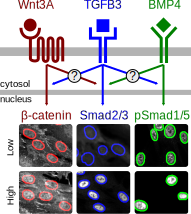
\includegraphics[width=3in]{FIGS/insulation/schematic.pdf}
  {\singlespacing 
  \caption[Schematic of the experimental system for \tgfbsf/Wnt crosstalk.]
        {Schematic of the experimental system for \tgfbsf/Wnt
         crosstalk. To measure inter-pathway signaling crosstalk,
         ligands can be applied combinatorially, followed
         by measurement of nuclear transcription
         factor levels. As shown, Wnt3A increases global
         quantities of \bcat, \tgf 3 causes translocation
         of bulk Smad2/3 to the nucleus, and levels of nuclear
         phospho-Smad1/5/8 increase upon BMP4 treatment.
         HCECs, with (``High'') or without (``Low'') 2hr treatment by
         Wnt3A (240ng/mL), \tgf 3 (4ng/mL), or BMP4 (73ng/mL).
         Outlines are of nuclei, segmented from the Hoechst channel
         (channel not shown) using the same threshold-segmentation method
         as in all imaging studies in this chapter.
         Fields are chosen to demonstrate visually obvious
         outcomes of signaling, though the diversity of responses
         is quite high for all pathways
         (see Figs. \ref{fig:insulation:ligandInformation} \&
         \ref{fig:insulation:readoutInformation}).}
  \label{fig:insulation:schematic}}
  \end{figure}
  

I reasoned that, because transcription factor activity is
the direct endpoint of signal transduction, I can infer the
degree of meaningful \tgfbsf\ and Wnt signaling interaction by measuring
how stimulation of one pathway affects the immediate transcription factor
response of the other pathway (\ar{fig:insulation:schematic}).
Current studies typically rely on transcriptional readouts to infer
such interactions, but these inferences may be confounded by transcriptional
feedback (which I consider to be the result of nuclear decision-making,
not signal transduction). Therefore, to accurately interpret cross-pathway effects
with respect to signaling, I use experimental timepoints that are
as close to the initial signaling event as possible.
Additionally, it is widely
believed that both Wnt and \tgfbsf\ signaling can be highly context-dependent.
I therefore repeat the experiments in this chapter using multiple
cell types, chosen to represent divergent cellular contexts.
By doing so, the hope is that any resulting shared properties of signal
integration can be more confidently extrapolated to other cellular systems.

In order to rigorously quantify single-cell responses to the
many experimental conditions required for this study,
and to make use of the expertise within the Altschuler \& Wu
lab, I use high-throughput immunofluorescence imaging as my primary
experimental platform. Unless otherwise indicated,
the presented measurements in this chapter originate from the
total-intensity feature values of individual nuclei. I typically report the
population-medians of these single-cell values, from replicate experimental
setups (as shown schematically
in \ar{insulation:system:measurement}; see \ar{imaging:introduction}
for more detail on my approach to image analysis).


  \begin{figure}[!bt]
  \centering
  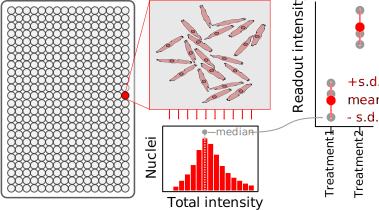
\includegraphics[width=3in]{FIGS/insulation/measurementSchematic.pdf}
  {\singlespacing 
  \caption[Schematic of the population-level fluorescence metric.]
        { 
        The fluorescence intensities reported in this
        chapter are population-level, based on single-nuclei
        measurements. As shown schematically here,
        cells are treated in
        96- or 384-well plates (left) and then fixed, immunostained,
        and imaged (middle, top).
        Nuclei are then identified computationally
        (see \ar{imaging:features}) so that the distributions
        of single-nuclei total fluorescence are obtained
        (middle, bottom). The medians of these distributions are
        then calculated for each replicate well. The reported
        values in this chapter are the means and standard deviations
        of these median values, nearly always from $n$=3 replicates.
        P-values are then calculated using an unpaired, two-tailed
        Student's t-test, and significant differences (p<0.05) are
        indicated with an asterisk. Figure legends indicate
        which samples are being compared for
        statistical significance.
        }
  \label{insulation:system:measurement}}
  \end{figure}
  

\subsection{Choosing cell types}
\label{insulation:system:readouts}


In order to choose useful cell lines, ligands, and readouts
for the study of Wnt and \tgfbsf\ signaling, I was confronted
with something of a chicken-or-the-egg problem. However, ongoing work
within the Altschuler \& Wu 
lab had made use of purified recombinant \tgf 1 for stimulating
the \tgf\ pathway and a total-Smad2/3 antibody for measuring the response.
Additional work had shown the efficacy of a \bcat\ antibody for
measuring cellular responses to purified Wnt3A. I therefore first made
use of these reagents, using literature-supported concentrations,
to identify cell lines that show responsiveness
to these pathways.


  \begin{figure}[!bt]
  \centering
  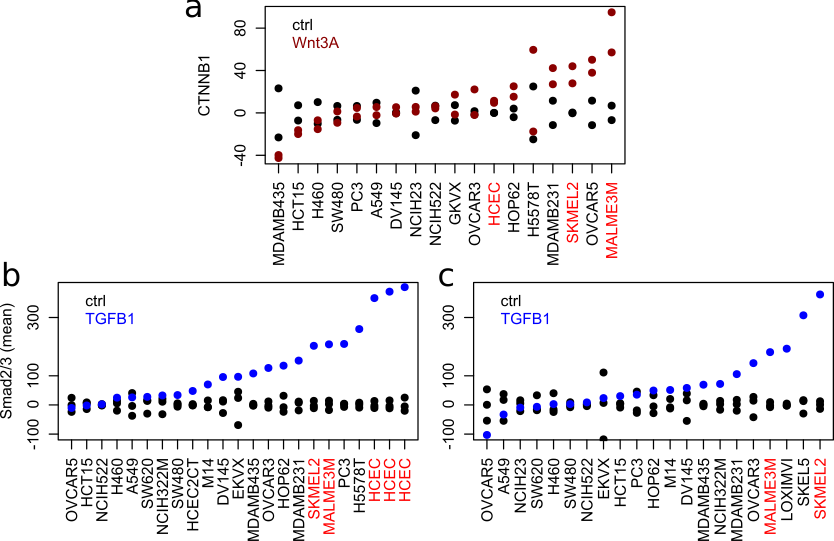
\includegraphics[width=6in]{FIGS/insulation/celltypeScreen.pdf}
  {\singlespacing 
  \caption[A screen for Wnt and \tgf\ responsive cell lines.]
        { A screen for Wnt3A (\b{a}) and
          \tgf 1-responsiveness (partial-replicate screens
          \b{b} and \b{c}) 
          across $\sim$20 cell lines revealed consistent
          responses by human colonic epithelial
          cells (HCECs) and two melanoma lines
          (SKMEL2 and MALME3M), highlighted with bright red text.
          The measured single-cell feature is the nuclear
          mean of fluorescence intensity by imaging
          (arbitrary units). Plots show the median
          of these single-cell values across all cells in
          a treated well (as in \ar{insulation:system:measurement}).
          The control means are subtracted from all values, per cell line,
          to show absolute changes in nuclear intensity.
          Concentrations: 1ng/mL \tgf 1, 200ng/mL Wnt3A.
          Timepoints: 1.25hrs (Wnt3A), 1hr (\tgf 1).
        }
  \label{fig:insulation:celltypeScreen}}
  \end{figure}


I first selected an immortalized (via telomerase and CDK4 expression)
but non-transformed human colonic epthelial cell (HCEC) line. This
cell line has stable ploidy and properties consistent with it being
a pseudo-differentiated cell type \cite{Roig2010}. Given the importance
of Wnt and \tgfbsf\ signaling in the gut (\ar{pathways:wntTgfb:gut}),
this cell line makes for a
reasonable model system for studying crosstalk between these pathways.
As a control, I also chose the rat small intestine
epithelial line (IEC6) \cite{Quaroni1978},
reasoning that it should display similar properties to HCECs.
I found that both of these
cell types respond strongly (in a statistical sense)
to TGFB ligands, moderately to BMP4,
and weakly (but measurably) to Wnt3A.


As discussed in \ar{introduction:encoding:context}, signaling
pathways generally show context-dependency, especially with respect
to differences in cell type. This non-generality is especially
true of the \tgfbsf\ and Wnt pathways (\ar{pathways:introduction}).
Therefore, in order to discover general properties (if indeed they exist)
we need to look for commonalities across cell types; the two intestinal
cell lines chosen may not be sufficient to infer generality. 
One approach to increase generality would be to
exhaustively test a large number of cell types, so that with each
successive cell type we gain confidence in the generality of a biological
phenomenon. Unfortunately, this approach is costly and difficult, and still
does not lead to certainty in the generality of a discovered phenomenon.
I opted then for a simpler approach, which is to test a small number of
divergent cell types. In this way, any behaviors consistent
across cell types can still be extrapolated as ``general'' behaviors,
though the resulting confidence in such a generalization may be somewhat
lower. 


To identify additional cell types for studying \tgfbsf\ and Wnt
crosstalk, I screened a panel of cancer cell lines for responsiveness
to \tgf 1 and Wnt3A. 
Additional selection criteria included cell morphology and
growth patterns that would allow for accurate image segmentation (see
\ar{imaging:features}), as well as cellular
growth rates and adherence properties that would
allow for the throughput needed for the many experimental conditions
required in my studies.
Two melanoma cell lines, SKMEL2 and MALME3M,
satisfied these criteria and were consistently ranked among the most
responsive to both \tgf 1 and Wnt3A (\ar{fig:insulation:celltypeScreen}).
Both of these cell lines can form malignant melanomas in nude mice, and
have abnormal ploidy  \cite{Fogh1977}. In particular, I found that SKMEL2 cells always
form tri-modal cell cycle distributions, implying the presence of diploid,
tetraploid, and octoploid cells within an asynchronous cycling population.
To my knowledge, there are no Wnt or \tgfbsf\ pathway mutations in SKMEL2
or MALME3M cells.


These cell lines should not be used to make
inferences with respect to differences between ``normal'' and cancer
cells, as these cell lines differ also in tissue of origin. Instead,
they should be thought of simply as divergent pairs of cell types that provide
consistent ``contexts'' (e.g. within the two intestinal lines or
within the two melanoma lines ) as well as divergent contexts (e.g.
between the intestinal and melanoma lines).
For all analyses in this chapter, I use only those cells
within the first peak of the imaging-based cell cycle distributions
(see \ar{imaging:variation:dnaQC}). I verified for each individual
pathway that the position of a cell within the cell cycle distribution
was not predictive of pathway behavior (data not shown) and
restriction to the G1/0 cell cycle phase otherwise reduces both experimental noise and
unimportant biological variation.
  
  
\subsection{Choosing signaling inputs and outputs}
\label{insulation:system:inputOutput}


Having chosen the cellular contexts in which to measure
the signaling crosstalk between \tgfbsf\ and Wnt, I then
needed to choose inputs and outputs that
could be believably interpreted to represent these pathways.
As discussed in \ar{introduction:encoding}, as a rule it
is not known what aspects of a signal or a readout are the
most relevant carriers of information for a cell. It is
generally believed, however, that for morphogenic pathways
it is the extracellular concentration of a ligand and the
nuclear concentration of a corresponding transcription factor that
are the relevant parameters. I therefore tested several ligands and readouts
in order to identify experimental inputs and outputs that are
both meaningful and practical.


  \begin{figure}[!bt]
  \centering
  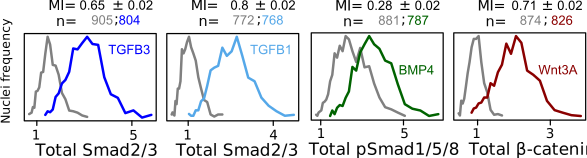
\includegraphics[width=6in]{FIGS/insulation/ligandInformation+.pdf}
  {\singlespacing 
  \caption[Information content of experimental treatments.]
        { Saturating ligand concentrations of \tgf 1/3 (12ng/mL), 
          Wnt3A (730ng/mL),
          and BMP4 (8ng/mL) are informative with respect to
          their canonical
          transcription factors. MI,
          mutual information between the ligand and readout
          (in bits, maximum MI is 1, see \ar{imaging:information}). 
          Histograms, distributions
          of single-cell total nuclear intensities for the
          immunostained transcription factors. $n$, number of cells
          per histogram, pooled from 3 replicate wells 
          (color-coded). Gray, untreated. 
          SKMEL2 cells, 1hr treatment. Arbitrary fluorescence units,
          frequencies scaled to have the same maximum value for display
          purposes.}
  \label{fig:insulation:ligandInformation}}
  \end{figure}
 
\subsubsection{Choosing prototypical ligands}
 
I first assayed several pathway inputs for information
content and signaling specificity. For the BMP2/4 pathway, I found that
all cell lines were non-responsive to purified BMP2 (data not shown) but
responsive to purified BMP4. These two ligands are
highly homologous and are thought to act through the same receptors
(\ar{pathways:tgfb:ligands}) therefore this absence of effective BMP2
signaling does not have a clear interpretation (perhaps a faulty reagent). In any event, the 
BMP4 signal is informative (using the mutual information metric,
as described in \ar{imaging:information});
the distribution of single-cell responses to saturating BMP4 is wide
but significantly different from the control distribution 
(\ar{fig:insulation:ligandInformation}). 


For the \tgf\ pathway I compared \tgf 1 and \tgf 3, as these ligands
are considered to be essentially interchangeable
(\ar{pathways:tgfb:ligands}). Indeed, within a single experiment
these two ligands generated similarly broad and separated Smad2/3
responses with similar mutual information
(\ar{fig:insulation:ligandInformation}). Dose-response curves for
the two ligands have the same
maxima and similar hill coefficients, though \tgf 3 is $\sim$10 time more
efficacious than \tgf 1 (data not shown).
\tgf 3 generally yielded more reliable responses, and so I use this
ligand for the remaining experiments in this chapter.


Finally, I chose to use purified Wnt3A to stimulate the canonical
Wnt pathway. Wnt3A is considered the prototypical ligand for this
pathway (\ar{pathways:wnt:wnt}), and its commercially-available
purified form has been widely used throughout the literature.
Importantly, I discovered that what is likely the most
commonly-used form, a low-purity ($\sim$75\%)
version from R\&D Biosystems, is sufficient to send Smad2/3 to the nucleus with the same
kinetics and dose-response Hill coefficicent as seen with \tgf\ treatment
(\ar{fig:insulation:contamination}a). I was unable to measure contaminating \tgf\ ligands
by Western (\ar{fig:insulation:contamination}b),
though this could be due to low concentrations of a high-efficacy \tgf\ variant.
In any event, this pathway crosstalk is likely
a consequence of trace amounts of contaminating \tgf\ in
the purified Wnt, as a pan \tgf-blocking antibody is sufficient to
block this response. Further, high-purity and carrier-free variants of the
product do not activate Smad2/3 (\ar{fig:insulation:contamination}c).


This artifactual crosstalk also occurs with the prototypical non-canonical
Wnt5A (\ar{fig:insulation:contamination}a,c), which casts
uncertainty onto recently-published work
linking Wnt5A and \tgf\ signaling
(reviewed in \ar{pathways:wntTgfb:dvl}) \cite{Miyoshi2012}.
The presence of such contamination may complicate the
interpretation of many other published studies, as it
suggests that treatment with purified Wnt3A or Wnt5A may generally include treatment
with \tgf, such that some resulting phenotypes 
could be due to stimulation by Wnt, \tgf,
or both.


  \begin{figure}[!bt]
  \centering
  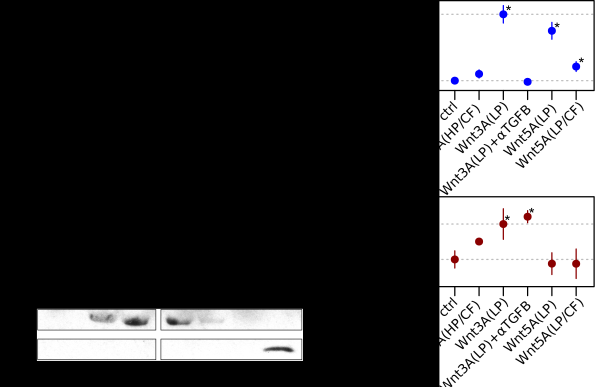
\includegraphics[width=5in]{FIGS/insulation/contamination+.pdf}
  {\singlespacing 
  \caption[Contamination of commonly-used commercial Wnt3A.]
        { The commonly-used low-purity (75\%) Wnt3A and Wnt5a ligands have
          trace amounts of contaminating \tgf.
          \b{a}, Dose-response curves
          for Wnt3A and Wnt5A against Smad2/3 yield EC$_{50}$ concentrations for
          the Wnts that are comparable to those used in the literature
          to stimulate Wnt responses (>100ng/mL is common).
          Duplicate experiments. Median of the mean nuclear
          intensity is plotted for each well (as in \ar{insulation:system:measurement}).
          \b{b}, Western blot of
          the purified Wnt3A ligands using a pan-\tgf\ antibody. HP/CF
          is the high-purity/carrier-free ligand used throughout this
          chapter, +BSA is the low-purity Wnt3A. BSA is shown as a reference.
          The low-purity Wnt3A lane should contain
          $\sim$25\textmu{g} of BSA in this blot, which is enough protein
          to soak up significant \tgf\ antibody.
          \tgf 1 is $\sim$12 kiloDaltons.
          \b{c}, The apparent Wnt$\rightarrow$Smad2/3 response is completely blocked
          by co-treatment with a pan-TGFB antibody that does
          not block the ability of Wnt3A to stimulate a \bcat\
          response. Low-purity Wnt5A also stimulates Smad2/3,
          but a carrier-free (CF) version does not. The high-purity (>90\%)
          carrier-free (HP/CF) Wnt3A shows a minimal Smad2/3
          response that is reproducible in other experiments, though not significant
          in this one. Concentrations: Wnt3A (200ng/mL),
          Wnt5A (100ng/mL), \textalpha{TGFB} (5\textmu{g}/mL).
          Y-axes and p-values as in 
          \ar{fig:insulation:specificity}.
          \b{a,c}, HCECs, 1hr treatment.}
  \label{fig:insulation:contamination}}
  \end{figure}

  
I therefore use high-purity/carrier-free Wnt3A for all experiments
in this chapter. I note, however, that even this ligand often causes
a small increase in Smad2/3 and so crosstalk experiments must be
interpreted with this fact in mind.

  
\subsubsection{Choosing prototypical readouts}


Having identified robust pathway inputs, I then needed to validate
antibody-based pathway outputs for immunofluorescence imaging.
For the \tgf\ pathway, which specifically activates Smad2/3,
and the BMP4 pathway, which specifically activates Smad1/5/8
(see \ar{pathways:tgfb:smads}),
I find that the nuclear fractions of both active phospho-protein and
total-protein levels can respond robustly to pathway activation.
However, it is unclear from the literature whether it is the total
concentration or the phospho-state concentration that encodes
extracellular ligand levels.


  \begin{figure}[!bt]
  \centering
  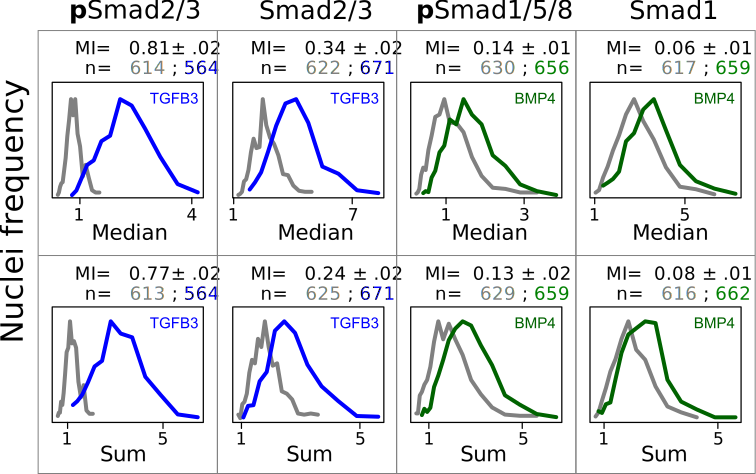
\includegraphics[width=5.5in]{FIGS/insulation/readoutInformation+.pdf}
  {\singlespacing 
  \caption[Information content of Smad readouts.]
        { Nuclear phospho-Smads (pSmads) contain more information about
          ligand concentrations than do nuclear total-Smads,
          though the sum and mean of intensity features are comparable. The
          untreated (gray) and treated (colored) distributions
          of single-nuclei measurements show more overlap
          of total-Smad readouts, resulting in relatively less mutual
          information (MI, in bits, maximum of 1, see \ar{imaging:information}).
          The median (top row) and
          sum (bottom row) of nuclear intensities for a single readout
          have nearly identical information content.
          $n$, number of cells
          per histogram (color-coded). 
          Ligand concentrations: saturating 10ng/mL
          \tgf 3 (blue) or 50ng/mL BMP4 (green).
          SKMEL2 cells, 1.5hr treatment. Arbitrary fluorescence units,
          frequncies normalized to have same maximum value.}
  \label{fig:insulation:readoutInformation}}
  \end{figure}


I therefore measured the mutual information
between these readouts and their ligands, which
revealed that the phospho-state is indeed more informative
(\ar{fig:insulation:readoutInformation}). Care should be taken when
interpreting this data, however, as the difference in information content
may also be due to antibody specificities, along with a myriad of
other causes. I note that
I have never observed maximum mutual information values of more than $\sim$1.2 bits
for any type of input/output relationship from imaging data, consistent
with published reports \cite{Cheong2011}.
The most fair statement, then, is that these particular approximations
of the phospho-state are more informative than these approximations of
total protein levels.


The total-Smad2/3 antibody yielded more-consistent
results across experiments than did the phospho-Smad2/3 antibody,
however, and has similarly-high
information content. I therefore use the total-Smad2/3
and the phospho-Smad1/5/8 (pSmad1/5/8) antibodies for the crosstalk experiments.
For canonical Wnt signaling there is strong evidence that it is the
total-protein level of \bcat, not the phospho-state, that encodes ligand concentration
(\ar{pathways:wnt:bcat}). I therefore use a total-protein \bcat\ antibody
to measure canonical Wnt responses.


\subsubsection{Validating input/output relationships}



  \begin{figure}[!bt]
  \centering
  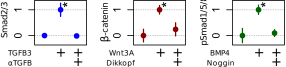
\includegraphics[width=4.5in]{FIGS/insulation/specificity+.pdf}
  {\singlespacing 
  \caption[Specificity of ligand/transcription factor relationships.]
        { The measured canonical transcription factor responses are a specific
          consequence of ligand treatment. \b{Left}, A
          pan-TGFB antibody (\textalpha{TGFB})
          blocks 2hr \tgf 3-induced
          nuclear Smad2/3 accumulation in HCECs. \b{Middle},
          Dikkopf, a soluble antagonist (\ar{pathways:wnt:frizzled}),
          blocks \bcat\ accumulation due to 2hr Wnt3A in
          SKMEL2s. \b{Right},
          Noggin, a soluble antagonist (\ar{pathways:tgfb:ligands}),
          blocks 1.5hr BMP4-induced phospho-Smad1/5/8 in SKMEL2s. Y-axes,
          median across single-cell nuclear intensities (the total feature)
          within a well. As in \ar{fig:insulation:schematic},
          points are the mean and standard deviation
          of $n=3$ replicate wells and `*' indicates one-sided p-value <0.05
          (Student's t-test) compared to control. Intensities normalized by
          $R_\text{i,norm}=\frac{R_\text{i}-\text{mean}(R_\text{ctrl})}
          {R_\text{ligand}-\text{mean}(R_\text{ctrl})}$.
          Concentrations: \tgf 3 (10ng/mL),
          \textalpha{TGFB} (5\textmu{g}/mL),
          Wnt3A (200ng/mL), Dikkopf (1\textmu{g}/mL),
          BMP4 (50ng/mL), Noggin (100ng/mL).}
  \label{fig:insulation:specificity}}
  \end{figure}
  
  
Aside from measuring the mutual information between each
input and output it is essential to ensure that
the input/output relationships are not artifactual. To do so, I verified
that each output could be blocked by a highly specific antagonist
\arp{fig:insulation:specificity}. 
Additionally, while I am primarily
interested in the signal transduction process, it is important
to ensure that a transduced signal leads to a nuclear decision.
In the case of \tgfbsf\ and Wnt signaling, this decision is
a change to the transcriptional network. The conserved
target for Wnt3A is Axin2, a negative auto-regulator
(\ar{pathways:wnt:bcat}). For \tgfbsf,
the conserved targets are the inhibitory-Smads (iSmads), Smad6/7
(\ar{pathways:tgfb:smads}). I therefore measured
mRNA levels of these transcriptional targets,
finding that stimulation does indeed yield transcription
in all cases (\ar{fig:insulation:expression}).


  \begin{figure}[!bt]
  \centering
  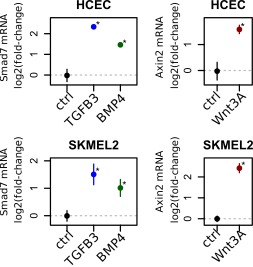
\includegraphics[width=3in]{FIGS/insulation/expression+.pdf}
  {\singlespacing 
  \caption[\tgfbsf\ and Wnt cause canonical target gene expression.]
        { The \tgf 3, Wnt3A, and BMP4 ligands cause
          expression of canonical target genes in the cell lines
          used in this dissertation. Fold-change
          is relative to the control condition. 2hr treatment. Concentrations:
          10ng/mL \tgf 3, 25ng/mL BMP4, 200ng/mL Wnt3A.
          Mean and standard deviation
          of 3 replicates, `*' indicates two-sided p-value <0.05
          (Student's t-test). mRNA levels measured by TaqMan qPCR
          (see \nameref{insulation:methods} for experimental details).
        }
  \label{fig:insulation:expression}}
  \end{figure}
  
 

  
  
\subsection{Interpretation of single-cell immunofluorescence measurements}


As for any method of measurement, it is important to
take a step back and think carefully about the biological
interpretation of the resulting data. For the image-based
single-cell data obtained in my work, cellular nuclei are
identified using Hoechst-staining and threshold segmentation,
and I only analyze those nuclei that likely belong to the G1 cell
cycle phase (see \ar{imaging:segmentation}).
Within these nuclei I tally up all pixel values to obtain
the total intensity feature, which I use as a proxy for
the quantity of the immuno-labeled target protein within the nucleus.
This feature and the mean intensity feature,
which is a proxy for concentration, are similarly informative
in my assays (\ar{fig:insulation:readoutInformation}), and
so I use the total-intensity feature for the practical
reasons described in \ar{imaging:totalIntensity}.
  

How do we interpret changes in this feature? Fold-change
over a reference (e.g. the untreated state) is a commonly used
metric, but the interpretation of fold-change is unclear in cases where
either the basal state is near zero (as any fold-change
value will move towards infinity) or is non-zero because of ``background'' signal
(which pushes all fold-change values towards 1). Using the
fluorescence image model that I present in 
\ar{imaging:model}, we can model the total intensity feature $T$
for any given nucleus $n$ by \ar{eq:system:total}. In this model the intensity of
each pixel $p$ is the sum of multiple fluorescence sources, such as
non-specific fluorescence ($F_{\text{nonspecific,}p}$,
e.g. due to off-target antibody
binding), non-signaling fluorescence ($F_{\text{nonsignaling,}p}$, 
e.g. due to a pool of the target
protein that is not involved in the studied signaling process), and the
actual signaling fluorescence $F_{\text{signaling,}p}$.
    %
    \begin{equation} \label{eq:system:total}
    T_n=\sum_p\left(F_{\text{nonspecific,}p}+F_{\text{nonsignaling,}p}+F_{\text{signaling,}p}\right)
    \end{equation}


Take the case of \bcat\ as an example. Basal
\bcat\ levels within Wnt3A-unstimulated cells are thought to be
essentially zero \arp{pathways:wnt:bcat}, and yet the measured basal levels are
quite high. This is due in large part to the presence of a
membrane-associated \bcat\ pool that does not participate in
Wnt signaling. It is impossible to know how the total nuclear
intensity breaks down into the various components of
\ar{eq:system:total}, and therefore
a metric like fold-change is uninterpretable in terms of the extent
of change for \bcat, though it can be used as a normalization method
to allow for measurements of relative change.


An alternative metric is to simply subtract a reference intensity measurement
from the experimental intensity, as the only term remaining will
be $F_\text{signaling,experiment}-F_\text{signaling,ctrl}$.
While this metric has a simple interpretation (absolute change in
signaling-associated fluorescence intensity), unfortunately it cannot be
used to infer the absolute magnitude
of response since fluorescence units are arbitrary.
Neither division nore subtraction can be used at the
single-cell level for fixed-cell assays,
as the relative contribution of each fluorescent component may vary
from cell to cell. Both metrics can be used
at the population level, however.


In summary, it is impossible to infer the absolute magnitude of change for
a signaling molecule using image-based immunofluorescence without
making assumptions that would be indefensible for the
immunofluoresce studies in this chapter. External
means of validation are then required to show that the observed
change is large enough to have a meaningful effect (as in
\ar{fig:insulation:expression}, where I show that the same experimental
treatments yield sizeable changes to target gene expression).
Relative comparisons between experimental perturbations are possible in any case,
and are easy to understand,
and so for convenience I use units normalized to a 0/1 scale throughout this chapter.


\subsection{Timepoints and concentrations}


Many studies of morphogenic signaling
pathways conflate the signal transduction and the transcriptional
decision-making processes due to use of long-term transcriptional
readouts. This conflation may be acceptable for some experimental
questions, but here my aim is to study integration specifically at
the level of signal transduction.


  \begin{figure}[!bt]
  \centering
  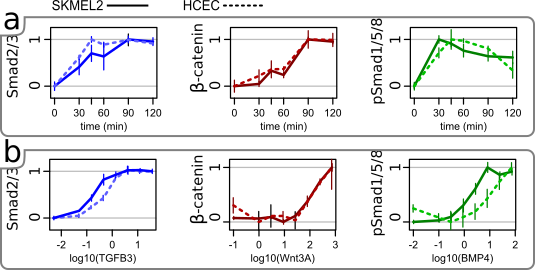
\includegraphics[width=6in]{FIGS/insulation/doseTime.pdf}
  {\singlespacing 
  \caption[Dose-response and timecourse of \tgfbsf\ and Wnt.]
        { The cell lines tested in this dissertation have similar
          but non-identical timelines (\b{a}) and
          dose-response curves (\b{b}). Shown
          are SKMEL2 (solid lines) and HCEC (dashed lines) cell lines.
          Cell lines show measurable responses between 60-120 minutes
          and are saturated by 10ng/mL \tgf 3, 1000ng/mL Wnt3A,
          or 100ng BMP4. Dose-responses are at 1hr.
          Y-axes as in \ar{fig:insulation:specificity},
          normalized so that the minimum and maximum responses
          are 0 and 1. Concentrations used in \b{a}:
		  TGFB3 (4ng/mL), Wnt3A (240ng/mL), BMP4 (70ng/mL).}
  \label{fig:insulation:doseTime}}
  \end{figure}
  

To do so, it is then necessary to minimize the effects of transcriptional
feedback on the stimulated pathways. I therefore performed
time-course experiments for each cell line and pathway in order to identify the
earliest timepoints that could still yield robust pathway responses
(shown for HCEC and SKMEL2 in \ar{fig:insulation:doseTime}a). For
all cell lines and pathways the responses were measurable by 1hr and
maximal by 2hrs, and so my crosstalk experiments take place within
this temporal window.
  

As I discuss in \ar{introduction:encodingSolution}, it is not necessarily true
that the use of a constant ligand concentration across multiple cell lines
is the appropriate way to ensure that the treatment is the ``same.'' Fortunately,
the dose-response curves for each cell line and pathway are not wildly different
(shown for HCEC and SKMEL2 in \ar{fig:insulation:doseTime}b) and so I was able
to determine concentrations that would yield approximately half-maximal responses (EC50)
or maximal responses across all cell types.


The reader may notice the use of differing ligand concentrations between
the experiments in this chapter.
For initial experiments, I did not yet know how responsive the cell types were
to each ligand, and so concentrations were based on prior work in the lab or
on literature-obtained values. For later experiments, doses were first chosen
according to whether a half-maximal or maximal response was experimentally
required, and these doses were then kept high over time to maintain saturating
levels in the face of slowly-degrading reagents and idiosyncratic sensitivities
of cell lines. Importantly, saturating concentrations
minimize the consequences of pipetting
error, since larger error can be tolerated before a measurable difference
in cellular responses will appear.



\section{Signaling integration between Wnt and \tgfbsf}
\label{insulation:wntTgfb}

Up to this point, the content of this dissertation has
all been designed to set up the question: To what extent
do Wnt and \tgfbsf\ interact during signal transduction,
prior to nuclear entry? As discussed throughout
\ar{pathways:introduction}, these pathways have extensive
opportunity for interaction and are widely believed to
integrate information at the level of transcription. Further,
despite a lack of shared core components, these signaling
pathways have been tied together by numerous studies
showing cross-pathway protein-protein
interactions \arp{pathways:wntTgfb:mechanism}. What is still unclear,
however, is whether these interactions take place and have
functional consequences to signal transduction under endogenous levels of
pathway components.


\subsection{Wnt3A and \tgf 3 show complete signaling insulation}


To measure the signaling crosstalk between \tgf\ and canonical
Wnt,
I made use of the experimental strategy described in the previous
section by treating cells with combinations of each ligand.
If these pathways
were to interact in a manner that affects signaling (i.e.
in a manner that transfers information) then
the direct outcome of signaling (that is, nuclear canonical
transcription factor levels) would be affected.


  \begin{figure}[!bt]
  \centering
  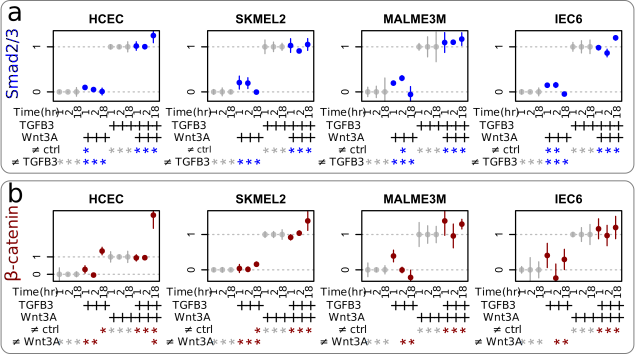
\includegraphics[width=6.5in]{FIGS/insulation/wntTgfbInsulation+.pdf}
  {\singlespacing 
  \caption[Wnt and \tgf\ are insulated during signal transduction (all data).]
        { Wnt and \tgf\ are insulated during signal transduction.
          \b{a}, Wnt3A causes little or no modulation of Smad2/3 responses at
          both short (1-2hr) and long (18hr) timepoints for all
          cell lines tested. \b{b}, \tgf 3 causes little or no
          modulation of \bcat\ responses, except in the case of
          long-term treatment in HCECs (note the 18hr \tgf 3 and 
          \tgf 3+Wnt3A responses). Y-axes and p-values as in
          \ar{fig:insulation:specificity}, with normalization per
          timepoint to set the control to 0 and the canonical-input-only
          condition to 1. These values fixed by normalization are in gray.
          $n=3$ replicates per point. p-values indicate
          whether each condition differs from control
          ($\neq$ctrl) or from the canonical-input-only
          condition (either $\neq$\tgf 3 or $\neq$Wnt3A).
          Concentrations (1 and 2hr): 0.2ng/mL \tgf 3,
          100ng/mL Wnt3A. Concentrations (18hr): 10ng/mL \tgf 3,
          200ng/mL Wnt3A.
          }
  \label{fig:insulation:wntTgfbInsulation}}
  \end{figure}
  

  \begin{figure}[!bt]
  \centering
  \includegraphics[width=5in]{FIGS/insulation/wntTgfb_summary.pdf}
  {\singlespacing 
  \caption[Wnt and \tgf\ are insulated during signal transduction (summary).]
        { Summary figure for insulation between Wnt3A and \tgf 3,
          limited to SKMEL2s and HCECs at 2 and 18hrs.
          \b{a}, At 2hrs, there is complete signaling insulation between
          Wnt3A and \tgf 3.
          \b{b}, However, context-dependent transcriptional integration
          already occurs at the same timepoint: HCECs show inhibition of
          Axin2 mRNA expression by \tgf 3 treatment, while SKMEL2s show
          complete transcriptional insulation.
          \b{c}, This context-dependent effect shows up at the level
          of signaling hours later, in HCECs. The increase in \bcat\ due
          to \tgf 3 signaling likely stems from the inhibition of Axin2
          mRNA (since Axin2 is a negative auto-regulator of Wnt3A). Thus,
          signaling insulation (\b{a}) combined with transcriptional integration
          (\b{b}) leads to a new, biased signaling state over time (\b{c}).
          Daggers
          indicate significant departure from pathway insulation.
          Data for \b{a} and \b{c} from \ar{fig:insulation:wntTgfbInsulation}.
          Data for \b{b} from \ar{fig:insulation:expressionXtalk}.
          }
  \label{fig:insulation:wntTgfbSummary}}
  \end{figure}
    

  
To test this, I treated all four cell types with combinatorial
inputs of \tgf 3 and Wnt3A, and then measured nuclear accumulation
of the transcription factors Smad2/3 and \bcat\ by
single-cell image analysis.
Data for all four cell lines are shown for 1, 2, and 18hr timepoints in
\arp{fig:insulation:wntTgfbInsulation}. This is a lot of data, and so
for simplicity I refer the reader to \ar{fig:insulation:wntTgfbSummary}, which shows
only the essential data for HCECs and SKMEL2s.


I performed the initial experiment at 1 and 2hr timepoints, using
ligand concentrations that ranged from EC50 to saturating across
the cell lines. In all cases, Wnt3A had small or
statistically insignificant effects on Smad2/3 levels, even when 
co-treated with \tgf 3 (\ar{fig:insulation:wntTgfbInsulation}a,
1 and 2hr timepoints; \ar{fig:insulation:wntTgfbSummary}a, top).
The small Wnt3A-induced Smad2/3 increases may be
real, but are likely due to the trace contamination discussed earlier
(see \ar{fig:insulation:contamination}). 
The same absence of signaling integration occurs in the other direction,
from \tgf 3 to \bcat\ (\ar{fig:insulation:wntTgfbInsulation}b,
1 and 2hr timepoints; \ar{fig:insulation:wntTgfbSummary}a, middle).
In this case, the presence of \tgf 3 had no significant effects
on \bcat\ levels in any context. Therefore, Wnt3A and \tgf 3 
are completely insulated during signal transduction
(\ar{fig:insulation:wntTgfbSummary}a, bottom).


Because the literature is full of examples of these two pathways interacting
over longer timescales, I decided to repeat the experiment with a more distant
timepoint.
To ensure that the absence of crosstalk was not due to low activity of the
pathways.
To my surprise, even at 18 hours there was almost no measurable modulation
of the transcription factor activity of one pathway by the other
(\ar{fig:insulation:wntTgfbInsulation}, 18hrs). There was
one exception, however: HCECs show \tgf 3$\rightarrow$\bcat\ interaction
(\ar{fig:insulation:wntTgfbSummary}c, middle). Indeed,
\tgf 3 treatment alone was sufficient to activate \bcat, and co-treatment
with Wnt3A yielded an approximately additive effect.


The complete absence of cross-pathway transcription factor modulation
at early timepoints strongly suggests that the Wnt3A and \tgf 3
signaling cascades are completely insulated from one another,
displaying no signaling crosstalk whatsoever
(\ar{fig:insulation:wntTgfbSummary}a, bottom). Further,
the frequent absence of cross-pathway modulation even given significant
time for transcriptional feedback shows that pathway insulation can be
maintained even after the transcriptional network has been remodeled by
morphogenic signals. Finally, the fact that HCECs lose this insulation
at later timepoints demonstrates a case of context-dependency
(i.e. dependency on cell type) in cellular decision-making
despite context-independent insulation of signal transduction
(\ar{fig:insulation:wntTgfbSummary}c, bottom).

  
\subsection{Wnt and \tgfbsf\ show context-dependent transcriptional integration}
 

Due to the surprising result that the direct outcomes of signaling
(transcription factor levels) are completely insulated between Wnt3A and \tgf 3,
I decided to test for insulation at the level of transcription. By
measuring mRNA expression 2hrs after treatment, I reasoned that I could
identify whether insulation at the level of signaling (as
already demonstrated) necessarily
implies insulation at the level of transcription. Because Axin2 and
Smad6/7 are the only prototypical transcription targets of the \tgfbsf\
and Wnt pathways, I measured mRNA levels of these genes following
combinatorial ligand treatment (\ar{fig:insulation:expressionXtalk};
simplified in \ar{fig:insulation:wntTgfbSummary}b).
 
 
  \begin{figure}[!bt]
  \centering
  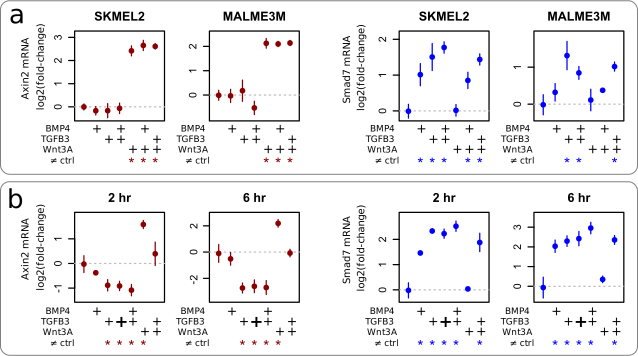
\includegraphics[width=6in]{FIGS/insulation/expressionXtalk.pdf}
  {\singlespacing 
  \caption[ Wnt and TGFB show context-dependent transcriptional crosstalk.]
        { Wnt and TGFB show context-dependent transcriptional crosstalk.
          \b{a}, In the melanoma cell lines, \tgf 3/BMP4 have no effect on
          Axin2 expression, while Wnt3A treatment has no effect on
          Smad7 expression. 2hr treatment.
          \b{b}, In HCECs, \tgf 3 reduces baseline and blocks
          Wnt3A-induced Axin2 expression. This effect is already apparent
          at 2hrs and is maintained at 6hrs. Wnt3A does not affect
          Smad7 expression in any context. Bold `+' indicates doubled
          \tgf 3 concentration, demonstrating transcriptional saturation of this pathway.
          Fold-change is relative to the control condition.
          Mean and standard deviation
          of 3 replicates, `*' indicates two-tailed p-value <0.05
          (Student's t-test).
          Concentrations: 10ng/mL \tgf 3, 25ng/mL BMP4, 200ng/mL Wnt3A.
          See \nameref{insulation:methods} for qPCR details.
        }
  \label{fig:insulation:expressionXtalk}}
  \end{figure}
  

By qPCR, neither of the melanoma cell lines show transcriptional
crosstalk between the canonical \tgfbsf\
and Wnt3A outputs Smad7 and Axin2
(\ar{fig:insulation:expressionXtalk}a), implying that these pathways
are insulated both in terms of the quantity of the transcription factors
sent to the nucleus (as shown in \ar{fig:insulation:wntTgfbInsulation})
and in the general activity of those
transcription factors. (This is not to say that these transcription factors
do not affect one another for any transcriptional targets.)
However, as before, HCECs display a different behavior.
By 2 hours HCECs show strong modulation of Axin2 expression
by \tgf 3 treatment(\ar{fig:insulation:wntTgfbSummary}b),
and this effect increases over time
(\ar{fig:insulation:expressionXtalk}b).


The modulation of Axin2 by \tgf 3 in HCECs is intriguing for
several reasons. First, it provides a simple explanation for the
18hr transcription factor modulation result observed in
(\ar{fig:insulation:wntTgfbSummary}c), since repression of Axin2,
a negative autoregulator of \bcat, could block the negative feedback
otherwise present after Wnt3A stimulation. Second, it clearly
shows that HCECs can simultaneously display signaling insulation
and transcriptional crosstalk,
demonstrating that these two processes can be completely
independent. Finally, the general lack of crosstalk across all
cell lines, coupled with the single instance of transcriptional
crosstalk in HCECs, is suggestive that the oft-cited idiosyncratic
outcomes of Wnt/\tgfbsf\ crosstalk are predominantly due to
context-dependent transcriptional crosstalk.



\section{Signaling insulation between BMP and \tgf}
\label{insulation:bmpTgfb}


 
  \begin{figure}[!bt]
  \centering
  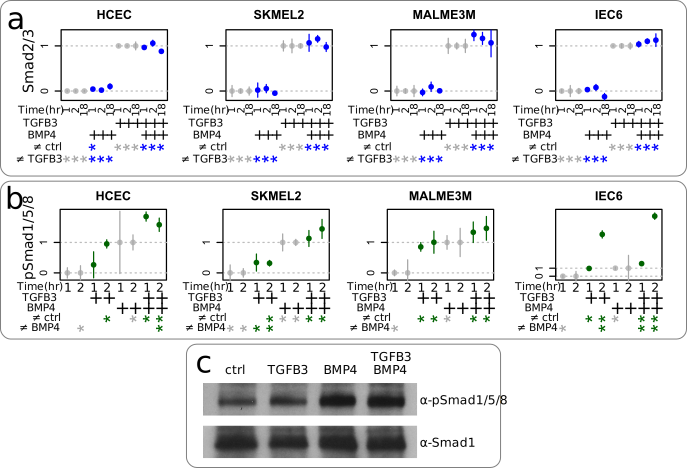
\includegraphics[width=6.5in]{FIGS/insulation/bmpTgfbInsulation.pdf}
  {\singlespacing 
  \caption[BMP4 and \tgf\ do not compete for Smad4 (all data).]
        { The \tgf\ and BMP signaling pathways are additive,
          and do not compete for Smad4. \b{a}, BMP4 causes no
          modulation of Smad2/3 responses at
          both short (1-2hr) and long (18hr) timepoints across all
          cell lines tested. \b{b}, \tgf 3 additively modulates pSmad1/5/8
          responses to BMP4. \b{c}, Measurement of \tgf 3/BMP4 crosstalk by
          Western is consistent with the imaging data. SKMEL2, 2hr treatment.
          \b{a,b}, Y-axes, normalization, and
          p-values as in \ar{fig:insulation:wntTgfbInsulation}. 
          Concentrations (1 and 2hr): 0.2ng/mL \tgf 3, 5ng/mL BMP4. Concentrations (18hr): 10ng/mL \tgf 3, 25ng/mL BMP4.
          Western courtesy Curtis A. Thorne (Altschuler \& Wu lab, UT
          Southwestern).
          }
  \label{fig:insulation:bmpTgfbInsulation}}
  \end{figure}



The above result is perhaps not so surprising,
that two pathways (Wnt3A and \tgf 3) lacking any shared core components do
not modulate one another during signal transduction. 
Under this rationale the BMP2/4 and \tgf 1/3 pathways
might then be expected to interact, given their shared requirement
for Smad4. Indeed, the claim of intra-\tgfbsf\ crosstalk 
via Smad4 competition has been cited in many reviews and papers,
but to my knowledge has not been directly tested
(\ar{pathways:tgfb:crosstalk}). I therefore
decided to use the same experimental setup as above to measure
the extent of crosstalk between BMP4 and \tgf 3
(\ar{fig:insulation:bmpTgfbInsulation}). The essential data is
again summarized in a simpler figure
(\ar{fig:insulation:bmpTgfbSummary}). If these pathways do 
compete for Smad4, then co-treatment with saturating concentrations
of both ligands (to maximize sequestration of Smad4) should cause one or
both pathways to be attenuated.

  \begin{figure}[!bt]
  \centering
  \includegraphics[width=5in]{FIGS/insulation/bmpTgfb_summary.pdf}
  {\singlespacing 
  \caption[BMP4 and \tgf\ do not compete for Smad4 (summary).]
        { Summary figure showing the lack of Smad4 competition between BMP4 and \tgf 3,
          limited to SKMEL2s and HCECs at 2hrs.
          \b{a}, There is additive signaling crosstalk from \tgf 3 to
          pSmad1/5/8, but not from BMP4 to Smad2/3.
          \b{b}, At the same time, the transcriptional output from the combined
          pathways also appears to be additive.
          \b{c}, Smad4 RNAi reduces protein levels of Smad4 in HCECs.
          Histone H3B serves as a loading control. 
          \b{d}, Smad4 RNAi in HCECs reduces overall \tgf 3 responsiveness (top)
          but not pSmad1/5/8 responsiveness (middle), while the signaling
          crosstalk between \tgf 3 and BMP4 remains approximately
          additive. Thus, competition for Smad4 does not cause cross-pathway
          signaling inhibition between \tgf 3 and BMP4. Normalization
          for \b{d} uses the control and single-ligand responses from
          the scramble siRNA treatment to define 0 and 1.
          Y-axes, normalization, and
          p-values as in \ar{fig:insulation:wntTgfbInsulation}. Daggers
          indicate significant departure from pathway insulation.
          Data for \b{a} from \ar{fig:insulation:bmpTgfbInsulation}.
          Data for \b{b} from \ar{fig:insulation:expressionXtalk}.
          Western courtesy Curtis A. Thorne (Altschuler \& Wu lab, UT
          Southwestern).
          }
  \label{fig:insulation:bmpTgfbSummary}}
  \end{figure}
    
  
  
BMP4 treatment
had absolutely no effect on Smad2/3 in any cell line
(\ar{fig:insulation:bmpTgfbInsulation}a;
 \ar{fig:insulation:bmpTgfbSummary}a,top). There is crosstalk
in the other direction:
treatment by \tgf 3 is sufficient to activate pSmad1/5/8, and
the presence of both ligands yields an additive behavior
(\ar{fig:insulation:bmpTgfbInsulation}b). Importantly, these
two pathways also have an approximately-additive effect on
transcription of their shared downstream target, Smad7
(\ar{fig:insulation:expressionXtalk}; \ar{fig:insulation:bmpTgfbSummary}b,top).
As noted
in \ar{pathways:tgfb:smads}, while the BMP2/4 and \tgf\ pathways
are generally considered to be distinct, they have been shown to
cross-activate one another in various settings.
Western blotting was not quantitative enough to confirm the
activation of pSmad1/5/8 by \tgf 3, but is consistent with an
absence of negative cross-regulation
(\ar{fig:insulation:bmpTgfbInsulation}c). In any case,
both the insulation of Smad2/3 from BMP4 and the additive
crosstalk between \tgf 3 and pSmad1/5/8 directly argue against
competitive inhibition between these pathways
during signal transduction.


I then wondered if the absence of inhibitory crosstalk
between BMP4 and \tgf 3 was a context-dependent phenomenon.
For example, the additive behavior is consistent
with the quantity of Smad4 being so high
as to be non-limiting, in which case both pathways would effectively have
distinct pools of Smad4 (as in \ar{fig:insulation:crosstalk}c).
I therefore used siRNA to knock down Smad4 in order to make Smad4 a
limiting factor in an effort to modulate the form of crosstalk
(e.g. to a non-additive form as in \ar{fig:insulation:crosstalk}d).


As a consequence of Smad4 depletion
(\ar{fig:insulation:bmpTgfbSummary}c), \tgf 3 signaling was strongly reduced overall
but was still not inhibited by co-treatment with BMP4
(\ar{fig:insulation:bmpTgfbSummary}d, top). Levels of pSmad1/5/8,
on the other hand, were not affected overall by Smad4 knockdown
(\ar{fig:insulation:crosstalk}d, top) and the effect of co-treatment
remained roughly additive. Therefore, in contrast to expectations,
BMP4 and \tgf 3 do not negatively regulate one another at all
at the level of signal transduction, and do
not compete for Smad4.



\section{Discussion}
\label{insulation:discussion}


In this chapter I measured the extent of crosstalk
between key morphogenic pathways, using a mechanism-independent
and endogenous approach that kept signaling crosstalk separable
from transcriptional crosstalk.
By doing so, I discovered that canonical Wnt and \tgf\
do not crosstalk at all during signal transduction, and that
\tgf\ and BMP do not compete for Smad4 during signaling.
Both of these results yield important simplifications to
the ever-increasing apparent complexity of signal transduction
that stems from discoveries of putative nodes of crosstalk.
Below, I discuss specific implications in more detail.


\subsection{Morphogenic signaling is insulated}


As I explain in \ar{pathways:discussion}, crosstalk during
signal transduction is likely to decrease the accuracy of the
intra-nuclear model of the extracellular environment. In such
a case, the information that eventually passes to the nucleus
for transcriptional processing represents a simplified view
of the cellular microenvironment, such that the nucleus then
has to make a decision with more uncertainty about the state of the outside world.
By instead allowing information to pass relatively unfiltered
from the extracellular milieu to the nucleus (e.g. by insulating
information channels from one another) the nucleus has access to a more
accurate model of the microenvironment and, presumably,
can then make more useful decisions.


The results presented in this chapter suggest that
the morphogenic Wnt and \tgfbsf\ pathways are indeed isolated
from one another, such that they can each pass information to
the nucleus without cross-pathway interference. As each pathway is only
capable of sending a small amount of information regarding
ligand concentration (not shown, but one can infer this from the broad distributions in Figs.
\ref{fig:insulation:readoutInformation} \&
\ref{fig:insulation:ligandInformation}), maintaining this
information from distinct pathways may be the only way
that a cell can obtain an accurate internal model of its
environment. Therefore, I propose that signaling insulation
may be a general property of morphogenic pathways whose
key outputs are changes to the transcriptional network.


Signaling insulation allows for the internalization of a
somewhat unfiltered view of the cellular microenvironment
(\ar{fig:insulation:wntTgfbSummary}a, cartoon).
Context-dependent transcriptional feedback
(\ar{fig:insulation:wntTgfbSummary}b, cartoon) can then modulate
the signaling pathways over time (either by auto-regulation or
cross-pathway regulation)
(\ar{fig:insulation:wntTgfbSummary}c, cartoon). The result of this nuclear
decision-making would be to essentially bias the
cell's view of what could even be an unchanging environment. Thus,
by mixing insulated signaling with long-term feedback,
cells can maintain a relatively complete internal model
of the environment but interpret that environment in a
temporally biased manner.


An obvious argument against general morphogenic insulation
in my own data is that \tgf 3 appears
to activate the BMP-specific Smads (Smad1/5/8). I note that
I was unable to verify that this crosstalk is specific (i.e.
not due to a contaminant) as addition of an anti-\tgf\
antibody along with \tgf 3 treatment did not significantly block
the interaction (data not shown). For this reason, I only
interpret the BMP/\tgf\ crosstalk data to say that one does not
inhibit the other.


An additional counter-argument is that these pathways
may in fact interact, but I have measured the wrong
thing to be able to identify the interactions. This would
be a useful discovery, as what my work shows is that
the generally-accepted method of encoding used by these
pathways shows complete insulation. It seems to me quite
possible that there exists some information channel, at
the level of signaling, that does indeed integrate information
from both Wnt and \tgf\ signals.


\subsection{BMP and \tgf\ do not compete for Smad4}


While it is widely believed that co-activation of the
BMP and \tgf\ pathways should result in some sort of
cross-pathway inhibition via Smad4 competition, I find
no evidence of this phenomenon. Indeed, I am unaware
of any studies that explicitly show this form of crosstalk,
and some studies have shown that Smad4 is highly
abundant \cite{Nicolas2004,Clarke2006}.


Interestingly, my data show that even when Smad4
is brought down to limiting levels, there is still no
cross-pathway inhibition. Smad4 is seen as
the factor that allows receptor-Smad (rSmad) access to
the nucleus, and it is generally believed that this
interaction is stoichiometric and non-transient \cite{Warmflash2012}. 
If this were the case, how could limitation of Smad4
selectively ablate one arm of Smad responses but not the other?


One possibility is that my observed difference between an
ablated Smad2/3 and maintained pSmad1/5/8 responses
(\ar{fig:insulation:bmpTgfbInsulation}e) is due
to some difference between the behavior of the bulk protein on one hand
versus the phosphorylated form on the other. However, such an effect would
be difficult to reconcile with the standard model that
the phospho-state allows Smads to stay in the nucleus
(i.e. the nuclear phospho- and total-protein levels should vary together).


What is, to me, a more likely explanation is that one of the
consequences of ablating Smad4 signaling, wich requires 48 hours
of transfection, is a change to the transcriptional network
with respect to \tgfbsf\ pathway components. For example, loss
of Smad4 may have resulted in a decrease in the quantity of \tgf\
receptors, co-receptors, or even an increase in secreted
antagonists. I did not test this, and therefore cannot make
a conclusion with respect to the differential effect of Smad4 RNAi
on Smad2/3 and pSmad1/5/8. Therefore, the most reasonable takeaway from this
data is simply that reduction in Smad4 does not force pathway
crosstalk.


The lack of competition for even low levels of Smad4 leads
to a potential modification of the current model of Smad
nucleo-cytoplasmic shuttling (see \ar{pathways:tgfb:smads}).
It may be that interactions of the
rSmads with Smad4 are more transient than is currently
believed, and that association with Smad4 is not required
for nuclear receptor-Smad activity and maintained localization.
In such a case, Smad4 could behave more like an enzyme
than a stoichiometric scaffold, in that single Smad4 molecules
could mediate the nuclear translocation of numerous rSmads.
If this process were fast enough, then the two classes of rSmads
would effectively have access to different pools of Smad4;
activity of one pathway would not ``soak up'' the co-Smad even
at pathway saturation.


\subsection{Future directions}


While this work has demonstrated that morphogenic
pathway integration may not be as complicated as we think,
there are many unanswered questions. Perhaps the most straightforward
questions to address are on the generality of morphogenic
insulation. Does insulation extend to other classic morphogenic pathways
(such as Hedgehog and Notch)? Does it extend to yet more
diverse cell lines than those tested here? I suspect that
signal transduction insulation is a general principle, and future
work using the approaches
in this chapter could provide the answers to these questions. 


It would also be informative to study the kinetics of crosstalk.
For example, in the case of HCECs, which show cross-pathway
modulation of transcription factors after 18 hours
(\ar{fig:insulation:wntTgfbInsulation}),
one could measure how much time is required after the
signal this crosstalk becomes apparent. Such data could be used
to determine how
long it takes for a cell to build a new, biased model of
its environment, and how stable that biased model is in the presence
of either a constant or changing signal.


Throughout this dissertation I have been harping on this
concept of information transfer, as we must always make
assumptions regarding which cellular and protein properties
are carrying signaling information. My data for Wnt and
\tgfbsf\ suggest that these pathways carry relatively little information
about absolute extracellular ligand concentrations. This lack
of information implies either that cells are terrible concentration
detectors or that we are not looking at the right encoding
relationship between these ligands and the internal cellular model of those
ligands. A comprehensive study designed to sort out the sources
of information, and the precise intracellular properties into which
that information is encoded, will be essential to our understanding
of how cells make decisions as a result of \tgfbsf\ and Wnt signals.








\section{Methods}
\label{insulation:methods}


The rationale and general methodology for image correction
and analysis are provided in \ar{imaging:introduction}.
Specific experimental details are provided in the image captions;
this section provides information that is
broadly applicable or more detailed than is appropriate for a figure legend.


\textbf{Cell culture.} 
I maintained all cells in
RPMI1640 (Cellgro \#10-040) with 5\% FBS
(Gemini Bio-Products \#100-106) with
antibiotics/antimycotics under standard tissue
culture conditions (37$^{\circ}$C, 5\% CO2). In preparation
for imaging, I plate $\sim 10^4$ cells per well
of a 96-well plastic plate (Corning \#353219) and a fifth
of that for 384-well glass plates (Nunc \#164586). I use
DMEM (Gibco \#11965-126) at the time of seeding when starvation
conditions are needed. In either case,
cells are left to adhere overnight before being treated the following day.
For treatments, I dilute recombinant protein into the same
media that the cells are grown in. The proteins used for treatment are
listed in \ar{table:insulation:proteins}.
Most of the plates used in this chapter are 384-well glass plates.
Human colonic epithelial cells were a kind gift from
Dr. Jerry Shay (University of Texas Southwestern, Dallas TX)
\cite{Roig2010}. The other cell lines were obtained from 
American Type Culture Collection (Manassas, VA).

   \begin{table}[!bt]
    \centering
	\footnotesize
    \caption[List of recombinant proteins.]
    { Recombinant proteins used in this chapter. 
      Vendors: CST, Cell Signaling
      Technology Inc (Danvers, MA); 
      Life, Life Technologies (Grand Island, NY);
      R\&D, R\&D Biosystems (Minneapolis, MN).
    }
    \label{table:insulation:proteins}
    \begin{tabular}{llll}
    \hline
    Protein   & Vendor & Catalog \# & Lot \# \\ \hline
    BMP4        & CST  & 4697    & \\
    DKK1        & R\&D & 5439-DK & SMR2713041\\
    Noggin      & R\&D & 6057-NG & \\
    \tgf 1      & Life & PHG9204 & \\
    \tgf 3      & CST  & 8425    & \\
    Wnt3A-LP    & R\&D & 5036-WN & RSK31 \\
    Wnt3A-HP/CF & R\&D & 5036-WNP/CF & SVH0813081 \\
    Wnt5A-LP    & R\&D & 645-WN    & \\
    Wnt5A-LP/CF & R\&D & 645-WN/CF & MCR4513111 \\
    \hline

    \hline
    \end{tabular}
    \end{table}


\textbf{Gene expression.}
I plated cells in 96-well plastic plates as above and left them to
adhere overnight before treatment the following day.
Each treatment was performed in triplicate wells.
I used an Ambion Cells-to-CT
kit (Life Technologies) to extract mRNA according to manufacturer instructions,
and passed these samples on to the UT Southwestern
Medical Center Microarray core facility for
cDNA library preparation and TaqMan qPCR. The samples were
given obfuscating identifiers and within-plate positions
so as to blind the core facility
to the treatments and replicates.
TaqMan probes (Applied Biosystems) comprised
Smad7 (Hs00998193\_m1), Axin2 (Hs00610344\_m1),
and 18S rRNA (Hs99999901\_s1).
The core facility returned the raw threshold cycle ($C_t$)
values for each probe/sample combination, which I first internally
normalized by 18S rRNA levels to yield
$C_{t(probe,norm)}=C_{t(probe)}-C_{t(18S)}$ and then 
converted these values to fold-change over control.


\textbf{RNA interference.}
I used a Dharmacon Smad4 siGENOME SMARTpool
(GE Life Sciences, \#M-003902-01) to ablate Smad4 in HCEC cells.
For transfection I used Lipofectamine RNAiMax
(Life Technologies) according to manufacturer instructions.
The transfection media was left on cells for 48hrs, after
which I replaced the media with fresh media for >2hrs prior
to experimental treatment.


\textbf{Western blots.}
SDS-PAGE and western blotting were performed using standard techniques.
I plated cells in 6-well dishes and treated them the following day.
After treatment, I washed the wells with ice-cold PBS
and then lysed with RIPA buffer (50 mM Tris (pH 8.0), 150 mM NaCl,
1\% NP40, 0.5\% deoxycholic acid, 0.1\% SDS, 0.5 mM EDTA)
containing protease and phosphatase inhibitors (Sigma Aldrich).
Antibodies used are shown in \ar{table:insulation:antibodies},
generally with 1:1000 dilutions
(the CST rabbit Smad4 antibody was used
for blotting).


\textbf{Immunostaining}.
All solutions are made in PBS
(Gibco \#70013). All wash steps are repeated 3 times with 0.1\%
Tween20 (Fisher \#BP337). Antibodies are diluted into 2.5\%
BSA (Fisher \#NC9871802). Cells are fixed in 4\%
paraformaldehyde (Electron Microscopy Sciences \#15710) for
10min, permeabilized with 0.2\% Triton X-100 (Sigma \#93443)
for 10min, then washed. I then incubate the samples overnight
at 4$^{\circ}$C with appropriate primary antibodies
\arp{table:insulation:antibodies}.
After washing, I secondary-stain for 2hrs at
room temperature with
added 2.5\textmu{g}/mL Hoechst. 
Finally, I wash the samples once more before
storing them in PBST for imaging.
For all experiments, I prepare
6-18 uniformly-fluorescing wells for measuring image
shading, using the same dissolved
secondary antibodies and Hoechst.


    \begin{table}[!bt]
    \centering
	\footnotesize
    \caption[List of antibodies.]
    { Antibodies used in this dissertation. Vendors: CST, Cell Signaling
      Technology Inc (Danvers, MA); BD, BD Biosciences (San Jose, CA);
      Abcam (Cambridge, MA); Life, Life Technologies (Grand Island, NY);
      R\&D, R\&D Biosystems (Minneapolis, MN).
      The indicated dilutions are for immunofluorescence unless appended
      with a `w' for Westerns. The appendix `b' indicates use as a blocking antibody.
    }
    \label{table:insulation:antibodies}
    \begin{tabular}{llllll}
    \hline
    Target     & Dilution & Source & Vendor & Catalog \# & Lot \# \\
    \hline
    Smad2/3     &  1/1000  & Rabbit &   CST & 8685   & 3         \\
    pSmad1/5/8  &  1/100   & Rabbit &   CST & 9511   & 8         \\
    \bcat\      &  1/100   & Mouse  &   BD  & 624084 &           \\
    Smad4       &  1/100   & Rabbit &   CST & 9515   & 4         \\
    Smad4       &  1/100   & Mouse  & Abcam & 3219   & GR94411-1 \\
    Smad1       &  1/100   & Rabbit &   CST & 6944   & 2         \\
    Smad2       &  1/100   & Rabbit &   CST & 5339   & 4         \\
    pSmad2/3    &  1/100   & Rabbit &   CST & 8828   &           \\
    H3B         &  1/1000w & Rabbit &   CST & 9715   &           \\
    \tgf 1-3    &  1/1000bw& Mouse  &  R\&D & MAB1835   & CCI1512031  \\
    AlexaFluor 546 Anti-Mouse IgG (H+L) &  1/1000 & Goat &  Life & A11003 & 1256168   \\
    AlexaFluor 488 Anti-Rabbit IgG (H+L) &  1/1000 & Goat &  Life & A11008 & 1470706   \\
    \hline
    \end{tabular}
    \end{table}


\textbf{Imaging.} I imaged all stained plates on a
Nikon Eclipse Ti-E2000 microscopes controlled by NIS
Elements version 4, with an Andor Zyla sCMOS 11-bit camera. I wrote custom
image coordinate-generating software in Python for increased
stage precision. To obtain the signal from the camera alone, I take
detector images at low exposure times with no light source.


\textbf{Image Correction.}
The background and shading correction
followed the pipeline described in \ar{correction:pipeline}
using custom Matlab software.


\textbf{Segmentation and quality control.} For
all analyses, I wrote a custom Matlab threshold segmentation algorithm 
to automate detection of nuclei using the
Hoechst fluorescence channel. 
I manually set filters for size and shape, by cell type, to remove objects that are
likely to be artifacts. For each nucleus, I then extract
its area (in pixels) and the total of all pixel intensities
for all imaged channels. Finally, I follow the DNA-based
quality control and single-cell regression-based correction
described in \ar{imaging:variation} using custom R software.
The resulting high-quality G1-phase cells are used for analysis.


\textbf{Mutual information measurement.} I implemented
the unbiased mutual information algorithm as described in
\cite{Cheong2011} and discussed in \ar{imaging:information},
using a custom Matlab script. 



\chapter{On quantitative imaging of single cells}
\label{imaging:introduction}

\section{Introduction}

Fluorescence microscopy is a
powerful tool for measuring single-cell properties, especially when sub-cellular
spatial resolution is required. With modern computing
power and robotics, we can now use this technology to amass large
quantities of image data and so study
cell biology with increasing breadth and depth. 
Accurate high-throughput imaging and image analysis of single-cell data across
large numbers of conditions is becoming routine in
some labs and will continue to become even more commonplace
as the technology simultaneously improves and becomes cheaper.
The availability of the technology has led, in recent years, to a boom
in large-scale microscopy studies of single-cell phenotypes
\cite{Neumann2006,Young2008,Feng2009,Houle2010,Held2010,Singh2010,Futamura2012}.
However, our ability to generate
microscopy data is outpacing our collective ability to
analyze and interpret it.


Fluorescence microscopy has been an experimental staple of biology for many years,
though it is still infrequently used for rigorous quantitative analysis. More often,
researchers use fluorescence imaging to demonstrate a particular phenotype
(as I do in \ar{fig:insulation:schematic}),
or to manually count the instances of a visually obvious
phenotype. Our own visual perception is notoriously prone to error, however,
as our brains can choose to perceive patterns that do not exist, thus
allowing for latent biases to affect how we manually tally the data.
As biologists we are often painfully aware of this problem,
and so there seems to be a general unease when it comes
to evaluating imaging data. We all know the joke that,
in published figures, ``representative image'' is a euphemism for
``the best image I could find.''


The distrust is understandable, as proper evaluation
of imaging data is a non-trivial task, and researchers
rarely publish enough details to even allow
for thorough evaluation in the first place. This problem is 
made worse by a lack of imaging and analysis standards, and by the
difficulty inherent to making large image-datasets publicly available.


Biological image
quantification is a difficult and generally unsolved problem \cite{Danuser2011},
and its various approximate
solutions tend to require a level of expertise in mathematics
and computer programming, and at least a cursory
understanding of microscopy optics. Importantly, it also requires expertise
in the experimental biology under study. Few, if any, biology training
programs prepare students for such broad practical knowledge.


Cell biologists, like myself,
are rarely trained in quantitative fields
and so we tend to rely on our colleagues
in analytical fields to do the quantitative work for us. Those analysts,
in turn, typically lean back on the biologists for understanding the
``what'' and ``why'' of the analysis.
Unfortunately, the large knowledge and language
asymmetry between biologists and analysts
creates steep communication barriers that are hard to break
down. Therefore, the full benefits to cell biology of careful
quantitative microscopy may be going untapped.


My own work relies almost entirely on imaging (\ar{insulation:introduction})
and, having spent so much time thiking about and performing image analysis,
I have come to prefer imaging over other methods not only for its efficiency
in measuring single-cell properties across large numbers
of conditions, but also because it provides a literal view into
the mysterious and beautiful world of the cell. I therefore hope that
careful single-cell image analysis will someday become as commonplace as Western
blots.


My overarching goal in writing this chapter is to provide
an image analysis resource that is both accessible
to classically trained biologists
and useful for analysts from non-biological fields
that may be preparing to move into the field. In general, I aim to provide careful
biological and analytical
reasoning for a subset of the many choices that must
be made with respect to
fluorescence imaging experiments. In specific, I focus
on dealing with
experimental and imaging artifacts and noise,
and how to choose biologically meaningful single-cell
measurements. The methods and rationale in this chapter
are used extensively in \ar{insulation:introduction}.



\section{Images as layers of fluorescence}
\label{imaging:model}


The goal of quantitative biological imaging, in overly general terms, is to perform
a set of meaningful mathematical operations on fluorescent images.
We therefore require a mathematical model of fluorescence images
to use as a reference when discussing image correction and analysis.
Note that the model I construct below is designed
to be intuitive with respect to cell culture microscopy,
and so it differs slightly from the
more general models that it is founded upon
\cite{Schultz1974,Madiset1998,L2000,Model2001}.


A fluorescence microscopy image $I$ can be thought of as
a series of fluorescing layers, each with its own distinct properties,
that add together to create the final image \arp{fig:imaging:layers}.
In this simple model, a fluorescence image is composed of multiple
\b{foreground} and \b{background} layers that come 
from distinct components of the sample.
(As described below, I use specific
definitions of these terms ``foreground'' and ``background''
that may differ from one's intuition.)
It is important to note that additivity is a special property
of fluorescence microscopy, as bright-field and other non-fluorescence signals do
not necessarily behave in this way \cite{L2000}.
Further, there are cases where the layers
of fluorescence will become non-additive,
as the fluorophores and the camera
will display non-linear behaviors in certain ranges \cite{Hiraoka1987}. 
The model I describe
here, and all analysis in this chapter, assumes that
all contributing components are behaving within their linear ranges.


  \begin{figure}[!bt]
  \centering
  \includegraphics[width=3in]{FIGS/imaging/layers.pdf}
  {\singlespacing 
  \caption[ Images as layers of fluorscence.]
            { A fluorescence image $I$ of a cell is the sum of
			distinct fluorescence layers. Here,
			$F_1$ is the foreground signal of interest, $F_2$
			is non-specific staining within the cell, and $B$
			is background fluorescence from the imaging surface.}
  \label{fig:imaging:layers}}
  \end{figure}

  
\subsubsection{Experimental image layers $F$ and $B$}


In this dissertation, foreground ($F$) refers
to any image layer that emits fluorescence in a spatially non-uniform manner
within an image; the layer is not ``flat.''
The most useful foreground layer is due to the specific binding of a
fluorescent probe to its target, as this layer is
likely the one that is under study.
Where my definition of ``foreground'' may diverge from others
is that I include spatially non-uniform fluorescence artifacts
as foreground layers. Such artifacts might include
non-specific cellular staining, cellular autofluorescence
(as for layer $F_2$ in \ar{fig:imaging:layers}), and staining artifacts
such as halos, bubbles, or bright puncta.
Many biologists refer to these artifacts
as ``background'', but I have a specific definition for this term as well.


Also specific to this dissertation, ``background'' ($B$) refers to any image
layer that emits fluorescence in a spatially uniform manner within an image
(e.g. layer $B$ in \ar{fig:imaging:layers}).
In other words, the layer is ``flat,'' aside from variation between
pixels due to measurement error.
Background layers may include reflections from the imaging
surface, autofluorescence from unbound fluorophore in the solvent, or fluorophore
that has adhered to the imaging surface.


Finally, all fluorescent image layers scale linearly
with excitation light intensity and
exposure time (again, so long as we are in the
linear range for all image components).
For convenience
we can fold excitation intensity and exposure time into a single term $t$, 
which I refer to simply as ``exposure.'' 
Taken together we get the (yet-incomplete)
image model in \ar{eq:imaging:simpleModel} that contains $n$ foreground
and $m$ background layers.
%
\begin{equation} \label{eq:imaging:simpleModel}
I = t \left( \sum_{i=1}^n F_i + \sum_{j=1}^m B_j \right)
\end{equation}


\subsubsection{Image modification by the microsope}

The model in \ar{eq:imaging:simpleModel} describes the fluorescing
layers of an image, but there are also non-fluorescent properties
of images.
In digital fluorescence microscopy, the camera typically has some
non-zero baseline value that I refer to as the ``detector value'' $D$.
This value is a constant and does not change with
exposure \cite{Goldman2005}.


  \begin{figure}[!bt]
  \centering
  \includegraphics[width=5in]{FIGS/imaging/components.pdf}
  {\singlespacing 
  \caption[ Components of a fluorescence image.]
            { A fluorescence image can be modeled by
            $I=D+S(F+B)$, where $D$ is the baseline detector value,
            $S$ is shading, $F$ is the foreground, and $B$ is the
            background. Here, synthetic images of two foreground
            objects demonstrate each of these
            components. Plots indicate pixel values along the white line
            drawn across the image as i \b{a}. \b{a}, Two foreground objects that
            vary 2-fold in intensity are shown. \b{b}, Addition of
            background reduces the apparent fold-difference between the
            two foreground objects, as does addition of the detector
            (\b{c}). \b{d} Shading distorts the foreground and background,
            but leaves the detector contribution unchanged.}
  \label{fig:imaging:components}}
  \end{figure}



Uneven illumination of the image by the light source,
which I refer to as ``shading'' ($S$),
is an optical problem inherent to microscopy
\cite{Hiraoka1987,Inoue1997,Murray2007,Fiolka2008}. Shading
is a consequence of how light moves through lenses and so it is
not just a property of wide-field microscopy,
though this is a common misconception: shading is also present in confocal
and total internal fluorescence (TIRF) microscopy \cite{Fiolka2008,Herbert2012}.


Shading can be interpreted as variation in relative
exposure as a function of position within the image.
In other words, $S$ modifies
$t$ in a pixel-coordinate dependent manner. Because fluorescence units
are typically arbitrary, in that their absolute values carry
no meaning, I simplify the model further by setting $t=1$
and dropping it from the equation
(note that analyses making use of varied exposure
times could also collapse $S$ and $t$ into a single term).
By including the $S$ and $D$ components,
and a noise term $\epsilon$ to absorb
experimental error, we get the complete model in
\ar{eq:imaging:fullModel}.


I simplify the model further by collapsing all
foreground and background layers into
single terms. The resulting image model in \ar{eq:imaging:simpleFullModel}
is used throughout this text.
This simplification is useful because the basic image
correction and analysis methods presented in this chapter do not
distinguish between foreground layers or between background layers.
It is useful to keep the multi-layer model in mind, however, as
it will help when trying to untangle the overall fluorescence behavior
of experimental images.
See \ar{fig:imaging:components} for a visual
demonstration of the simple model. 


\begin{gather}
I = D + S \left( \sum_{i=1}^n F_i + \sum_{j=1}^m B_j \right)\epsilon  \label{eq:imaging:fullModel} \\
I = D + S (F+B)\epsilon  \label{eq:imaging:simpleFullModel}
\end{gather}


\subsection{Properties of the image components}


With a model in place, it is useful to obtain some intuition for how to
think about images in this framework. First, note that the image itself,
and each layer that makes it up, is a matrix of intensity values
(\ar{fig:imaging:stack}). Many
analytical operations can be performed per pixel coordinate, in effect
ignoring the presence of neighboring pixels.
Other operations take into account
those neighbors (this is especially true of segmentation,
discussed later). Finally, we can think of a ``stack'' of images,
in the same way
one would stack a deck of cards. We can perform operations ``down the
stack'' at particular pixel coordinate.
Such operations include ``per-pixel'' means and medians.


  \begin{figure}[!bt]
  \centering
  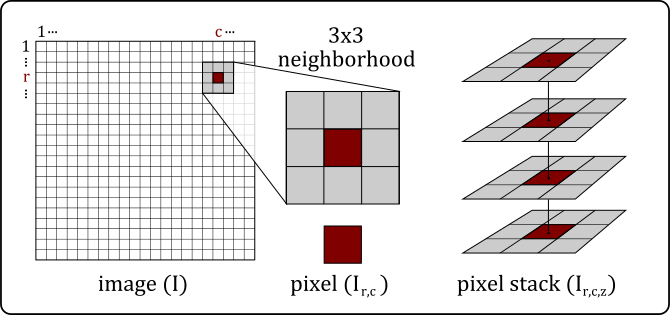
\includegraphics[width=4in]{FIGS/imaging/stack.pdf}
  {\singlespacing 
  \caption[ Pixel coordinate system.]
            { An image $I_{r,c}$ is a matrix of intensity values,
            with pixel coordinates
			given by row $r$ and column $c$. Analyses can
			be performed on single pixels, the entire image, image
			neighborhoods, or image stacks as shown. In the case of an image stack,
			$z$ refers to the image position within the stack. Note that $z$ need not
			refer to a height, as in the common z-stacks of confocal microscopy,
			but can also indicate different color
			channels or even entirely unrelated images. In effect, $z$
            is a ``height'' within the image stack that may not
            correspond to the physical height of an imaged within a sample.}
  \label{fig:imaging:stack}}
  \end{figure}


Each component of the image model in \ar{eq:imaging:simpleFullModel}
is a matrix of the same dimensions,
and each has distinct properties. The foreground components
of $F$ have completely idiosyncratic
values, both within and between images, as these
values depend on where cells are, what is
being stained, and what kinds of randomly-positioned
artifacts are present. Indeed, the
unknown behaviors of the foreground layers are 
what we typically aim to understand
via image analysis.


The background layers of $B$ are defined to
be more predictable, in that they are
unchanging by position within an image. The background should
be constant between images as well,
when identical experimental conditions
are used to obtain those images.
However, the total background
may change as a consequence of some experimental
perturbation. For example, some small
molecules used as drugs may fluoresce
and so add an additional background layer.
Finally, note that due to shading these
``flat'' background layers will appear
distorted in uncorrected images.
To clarify, then, I define background
layers as those that are constant across an image
in the absence of shading.


The detector layer $D$ has the simplest behavior, as it can be considered
constant regardless of the imaging and experimental conditions. ``Constant'' in this
case means that the value at any given pixel position $D_{r,c}$ does not change
over time or between images.
The values within an image, on the other hand, may vary
(see \ar{fig:imaging:properties}a).


The shading value $S$ is problematic for analysis in that it distorts the
$B$ and $F$ layers in non-trivial ways.
Like $D$, this layer also shows variation within an image.
The shading pattern caused by the objective lens
tends to show brighter fluorescence at image centers
and weaker fluorescence at the edges. However,
the presence of other components
in the light path, such as filters, can modify this shading pattern
(\ar{fig:imaging:properties}b) \cite{VandenDoel1998}.
Unlike $D$, the shading pattern can vary between
images as well, though in \ar{imaging:correction} I show that this variation
can be both predictable and correctable. $S$ distorts the $F$ and $B$ layers
multiplicatively, and can cause as
large as 1.5- to 2-fold intensity differences across an image
\cite{Bray2013}.




  \begin{figure}[!bt]
  \centering
  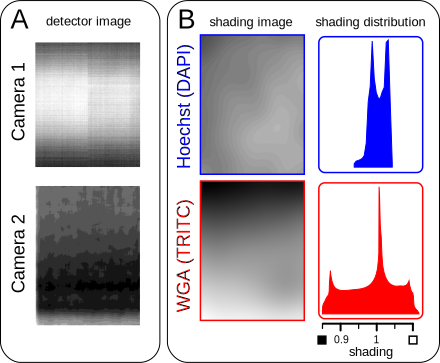
\includegraphics[width=4in]{FIGS/imaging/properties.pdf}
  {\singlespacing 
  \caption[ Example detector $D$ and shading $S$ patterns.]
            { Example within-image variation of the detector $D$
			and shading $S$ image components. \b{a}, Per-pixel
            averages of 10 detector images from
			two cameras are shown. Camera 1, Andor Zyla sCMOS 11-bit.
			Camera 2, Roper Scientific CoolSnap HQ2 CCD 14-bit.
            Intensities and
			images are scaled independently.
			\b{b}, Shading patterns from two optical channels. Uniformly-fluorescent
			background images were made with dissolved Hoechst or wheat
			germ agglutinin (WGA)-TRITC in the DAPI and TRITC optical channels. Note
			that each channel has a dramatically different shading pattern and overall
			degree of shading. Histograms show the all-pixel distributions
			of shading values, which are defined to have
			a median of one (a robust variant of $\E[S]\equiv 1$, defined in
			\ar{imaging:correction}).
			}
  \label{fig:imaging:properties}}
  \end{figure}


Finally, we are left with the noise term $\epsilon$. I use this
term specifically to capture measurement noise, not true biological
variability. The largest source of measurement
noise for modern fluorescence imaging
is probably due to the combination of two factors: the error in converting
photon counts to electrons, and the error introduced during transmission
of those electrons from the camera. Combined, this measurement error
introduces an intensity-dependent uncertainty in the total measured
intensity of the pixel $I_{r,c}$. In general, the relative error
decreases as a function of the square root of intensity \cite{Goldman2005}.




\section{On image correction}
\label{imaging:correction}

Fluorescence microscopy images contain non-biological data,
distortions, and artifacts that may confound analytical results if
not addressed.
In the terms of the image model from the previous section
(\ref{eq:imaging:simpleFullModel}), the
subject of study in fluorescence imaging is contained within a subset of the
foreground layers. All non-foreground components should thus
be removed in order to obtain meaningful quantitative results.
Ideally, the foreground layers that are not of interest (especially
artifacts) should also be removed, though this is a much more difficult
problem that I do not address in this dissertation.
In essence, from the original image $I=D+S(F+B)\epsilon$, we need to
obtain $F$: obtaining $F$ is the goal of image correction.


It is important to be aware that image correction is not a solved
problem. There are many ways in which it can be done, several of which I review
in \ar{imaging:correction:review}, but the most commonly-used methods produce
incomplete correction and/or are prone
to generating artifacts. Further, methods sections of papers that
rely on imaging often do not explain their correction methodology
at all, making it difficult to evaluate some published results.
I therefore make the importance of image correction a focus
of this chapter, and describe an image correction
approach that I developed for accurate determination of $F$
in the difficult context of high-throughput microscopy
\ar{imaging:correction:myMethod} \cite{Coster2014}.


Before going into the details of image correction, I should
first address whether this step is even necessary.
After all, any processing step
could introduce artifacts and thus potentially do more harm than good.
Normal cell-to-cell variability is already relatively high,
with standard deviations of 
$\sim$15-30\% for protein concentrations \cite{Sigal2006a}. One might then
wonder whether error introduced by non-foreground image components
would make much of a difference. Here I show that it can
indeed make a difference. Unsurprisingly,
the size of the difference (and thus the importance) is highly
dependent on the properties of each particular image dataset,
the measurement methods used, and the experimental goals.


\subsection{Non-foreground components distort single-cell phenotypes}
\label{imaging:distortion}


A particular cellular phenotype can be represented
as a set of measurements.
For example, a cell phenotype might be composed of
its measured size, shape, texture,
and average fluorescence intensities in multiple
color channels. Each measurement is
generally referred to as a ``feature.'' The diversity
of features that can be measured
for a  single cell is only limited by the imagination
of the investigator. It would therefore
be impossible to develop a single
comprehensive argument for the importance
of image correction that covers all possible
ways of measuring cellular phenotypes.
Instead, I make a case study of several
commonly-used and biologically-interpretable
single-cell features: the average, total,
and ratios of fluorescence intensity.


    \begin{table}[!bt]
    \caption[Table of symbols for average, total, and ratiometric features.]
    {Symbols used in the mathematical derivations of the consequences of $S$
    and $B$ on single-cell feature distributions.}
    \label{table:imaging:symbols}
    \centering
    \begin{tabular}{cl}
    \hline
    Symbol & Meaning \\ \hline
    $\E[X]$   & Expected value (i.e. the mean) of the random variable $X$ \\
    $F_c$	 & Average foreground intensity within cell $c$ \\
    $S_c$	 & Average shading value within cell $c$ \\
    $B$	     & Background intensity per pixel, a constant\\
    $\alpha_c$ & Area of cell $c$ \\
    $A$	     & Average intensity feature \\
    $T$	     & Total intensity feature \\
    $R$	     & Ratio of intensities feature \\
    $Z_c$    & The value of feature $Z$ for a single cell, $c$.\\
    $\sigma_Z$ & The standard deviation of feature $Z$ across all cells. \\
    $\mu_Z$    & The mean of feature $Z$ across all cells. \\
    $cv_Z$     & The coefficient of variation of feature $Z$ across all cells  ($\sigma_Z/\mu_Z$). \\
    \hline
    \end{tabular}
    \end{table}


How to quantify the effects of image correction on data is not obvious,
since that data can be used in many ways depending on experimental goals.
There are, however, aspects of
single-cell distributions that are meaningful across a broad array of
experiments, and so I use these as metrics when measuring the consequences
of image correction. These are the mean ($\mu$), standard deviation ($\sigma$),
and coefficient of variation ($cv=\sigma/\mu$) of a feature across a population of cells.


The standard deviation and $cv$ are measures of distribution widths, which
are used to determine the statistical separability of distributions.
Inaccurate measurements of the true variability may
consequently reduce statistical power.
The mean of a feature distribution, on the other hand,
is typically used to determine how large of an
effect an experimental perturbation has had. Inaccurate measurements of the true mean
may cause strong results to appear weak, or vice versa, leading to false
negatives or false positives. These distribution metrics are
therefore useful as readouts for the utility of image correction.


The mathematics in the following discussion were
worked out in conjunction with my co-authors on the relevant
publication \cite{Coster2014}: Satwik Rajaram, Chonlarat Wichaidit,
Steven Altschuler, and Lani Wu. The text
and figures draw heavily from the same publication. Those readers
who do not need convincing that image correction is important may skip
to page~\pageref{imaging:correction:review} without a loss in coherence
of this chapter.


  \begin{figure}[!bt]
  \centering
  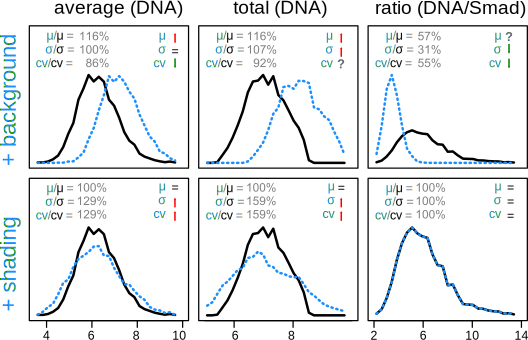
\includegraphics[width=4.5in]{FIGS/imaging/SBeffects.pdf}
  {\singlespacing 
  \caption[ Case study of the effects of $S$ and $B$ on single-cell features.]
            { Image background and shading cause feature-dependent changes
            in estimates of phenotypic variability.
            Human colonic epithelial cells ($n>3700$), stained for DNA
            (using Hoechst) and Smad (using a Smad2/3 antibody), imaged
            at 10X.
            The distributions of
            nuclear feature values were then compared
            before (black histograms) and after (dotted blue histograms)
            artificial background (top row, with
            background $\sim$16\% of Hoechst or $\sim$50\% of Smad foreground)
            or shading (bottom row, linear
            gradient with maximum 1.5 fold intensity difference) were added
            to each image. $\mu$, mean; $\sigma$, standard deviation;
            $cv=\sigma/\mu$. Inset, top left,
            relative size of change to the shown distributions. Inset, top right,
            arrows indicate the direction of
            change in the general case (question marks indicate uncertainty due to
            dependency on other variables). $x$-axes in arbitrary fluorescence units.
            A version of this figure is published as Fig. 1a in \cite{Coster2014}.}
  \label{fig:imaging:SBeffects}}
  \end{figure}





\subsubsection{Mathematical definitions of commonly used single-cell features}


Commonly used single-cell measurements include pixel intensity averages,
totals, and ratios within some cellular compartment $c$ (such as the
nucleus, cytosol, or whole cell).
By defining these features mathematically we
can determine their general behaviors as a consequence of the presence of image background
or shading. Refer to \ar{table:imaging:symbols} for the list of mathematical
symbols, to \ar{table:imaging:properties} for a summary of the statistical
properties used in the mathematical derivations, and
\ar{fig:imaging:SBeffects} for a case study of these behaviors.


For each cellular object, I define $F_c$ and $B_c$ as the average foreground
and background intensities within $c$, while $S_c$ is the
average shading. $B_c$ is a constant for all cells,
as the background is assumed to be the same for all
pixels in the absence of noise, and so I drop the subscript from this term.
I refer to the area of each cell, measured in pixels, as $\alpha_c$.
Finally, for the derivations I assume that the detector value has
been subtracted from all pixels
and that the image contains no measurement noise  ($D=0$
and $\epsilon=1$).


For each cell I can then define the three simple intensity features: total intensity $T$,
average intensity $A$, and the ratio of intensities $R$ between two independent foreground
signals $F_{c1}$ and $F_{c2}$ (e.g. the ratio of nuclear Hoechst and Smad intensities, as in
\ar{fig:imaging:SBeffects}). Because the ratio takes two signals into account, each may
come from a distinct fluorophore and optical setup and so have 
distinct shading and background values. Additionally, those features could be
defined within distinct cellular compartments, such that the compartment
sizes may also differ.
The three features are thus defined for single cells by 
Equations~\ref{eq:correction:average}\nobreakdash-\ref{eq:correction:ratio}.
	%
	\begin{align}
	A_c & = S_c (F_c+B) \label{eq:correction:average}\\
	T_c & = \alpha_c A_c = \alpha_c S_c (F_c+B) \label{eq:correction:total}\\
	R_c & = \frac{ \alpha_{c1} S_{c1}(F_{c1}+B_1) }{ \alpha_{c2} S_{c2}(F_{c2}+B_2) }  \label{eq:correction:ratio}
	\end{align}
	

For simplicity of the following analysis, I take the special case where
$F_c$, $S_c$, $\alpha_c$, and $B$ are all
statistically independent (i.e. cells do not
spatially arrange themselves within an image
by phenotype, and foreground intensity is
independent of cell size). Further, I
assume that cells are small relative to the
spatial rate of change of $S$ across an image.
These assumptions 
allow me to use the properties in
\ar{table:imaging:properties}. Note that these assumptions
will be valid for some experimental cases, but
certainly not all. For the case study
shown in \ar{fig:imaging:SBeffects} they are appropriate:
I verified that nuclear size and staining intensity
were uncorrelated with each other and with position, and that the two
foreground signals (Hoechst and Smad2/3) are independent (data not shown).


Finally, I noted earlier that units of fluorescence are typically arbitrary
and that $S$ causes a multiplicative change in relative intensity across
an image. This means
that we are free to choose how to define the expected value of $S$: a
value other than 1 would cause a scaling of the foreground and
background values, but this scaling would retain the relative relationship between
all measured intensities and so would be of no consequence.
For convenience, then, I define shading so that
its expectation value across all images and pixels is $\E[S]=1$
so that, for a large number of cells, $\E[S_c]\approx 1$. This definition simplifies
the mathematical derivations below, as the $\E[S_c]$ term can be dropped
from several formulae.


    \begin{table}[!bt]
    \centering
    \caption[Table of useful statistical properties.]{
    Statistical properties used in the derivations of the effects
    of shading $S$ and background on the distributions of single-cell
    average $A$, total $T$, and ratio $R$ intensity features. $X$ and $Y$ are independent
    random variables, and $k$ is a constant.}
    \label{table:imaging:properties}
    \begin{tabular}{ccl}
    \hline
    Index & Property \\ \hline
    1 & $\E[S_c] \equiv 1$  \\
    2 & $\mu_{X+k} \equiv \E[X+k] = \E[X]+k$ \\
    3 & $\mu_{XY} = \E[X]\E[Y]$ \\
    4 & $\sigma^2_X \equiv \Var[X] = 
        \E[X^2]-\E[X]^2 \implies \E[X^2]\geq \E[X]^2$\\
    5 & $\sigma^2_{[X+k]} = \sigma^2_X$ \\
    6 & $\sigma^2_{XY} = \E[X^2]\E[Y^2]-\E[X]^2 \E[Y]^2$ \\
    \hline
    \end{tabular}
    \end{table}



\subsubsection{Effects of background $B$ on the average intensity feature $A$}


For this case, we ignore the effects of $S$ and focus on $B$. 
We therefore set $B>0$ and $S_c=1$, so that the average feature 
from \ar{eq:correction:average} simplifies to $A_c=F_c+B$.
This results in the distribution properties for this feature in 
Equations~\ref{eq:correction:bamu}\nobreakdash-\ref{eq:correction:bacv}.
	%
    \begin{align}
    \mu_A    & \equiv \E[A_c] = \E[F_c+B] = \E[F_c] + B  \label{eq:correction:bamu}\\
    \sigma_A & \equiv \sqrt{\Var[A_c]} = \sqrt{\sigma^2_{F_c+B}} = \sigma_{F_c} \label{eq:correction:basd}\\
    cv_A     & \equiv \frac{\sigma_A}{\mu_A} = \frac{\sigma_{F_C}}{\E[F_c]+B} \label{eq:correction:bacv}
    \end{align}


It is clear that $B$ will always cause
an increase in the mean of average intensities, $\mu_A$ \arp{eq:correction:bamu}.
The standard deviation, $\sigma_A$, is
unaffected by background (\ar{eq:correction:bamu}, using Property 5 from \ar{table:imaging:properties}).
As a consequence of the
constant $\sigma_A$ and increased $\mu_A$, the coefficient of variation
will decrease with increasing background. In summary, background will cause
an overestimation of $\mu_A$, an underestimation of $cv_A$, and will not affect
$\sigma_A$ (ee the case study in \ar{fig:imaging:SBeffects}, top left panel).


\subsubsection{Effects of background $B$ on the total intensity feature $T$}


The situation is the same as the previous case,
except with the inclusion of cell size.
The total intensity feature \ar{eq:correction:total}
therefore simplifies to $T_c=\alpha_c (F_c+B)$,
resulting in the distribution properties shown in 
Equations~\ref{eq:correction:btmu}\nobreakdash-\ref{eq:correction:btcv}.
	%
    \begin{align}
    \mu_T    & \equiv \E[T_c] = \E[\alpha_c(F_c+B)]=\E[\alpha_c](\E[F_c]+B) =
        \E[\alpha_c]\E[F_c]+\E[\alpha_c]B
        \label{eq:correction:btmu}\\
    \sigma_T & \equiv \sqrt{\Var[T_c]} = \sqrt{\sigma^2_{\alpha_c(F_c+B)}} =
        \sqrt{\sigma^2_{\alpha_c F_c} + 2\sigma^2_{\alpha_c}\E[F_c]B
        + \sigma^2_{\alpha_c}B^2}
        \label{eq:correction:btsd}\\
    cv_T     & \equiv \frac{\sigma_T}{\mu_T} =
        \frac{ \sqrt{\sigma^2_{\alpha_c F_c}+2\sigma^2\E[F_c]B+ \sigma^2_{\alpha_c}B^2 } }
        { \E[\alpha_c]\E[F_c] + \E[\alpha_c]B }
        \label{eq:correction:btcv}
    \end{align}

    
Though somewhat less obvious than for the average feature,
it should be clear that increasing $B$ will cause
an increase in the mean of total intensities, $\mu_T$
(\ar{eq:correction:btmu}, using Property
3 from \ar{table:imaging:properties}). Importantly,
each cell will be affected differently by background, depending on its size.
Unlike the average feature, the standard deviation $\sigma_T$
increases with background (\ar{eq:correction:btsd},
using Properties 3 \& 6 from \ar{table:imaging:properties}).


Because both $\sigma_T$ and increased $\mu_T$ increase with
increasing $B$, it is not immediately obvious what the effect should be on the
coefficient of variation, $cv_T$ (as the numerator and
denominator in \ar{eq:correction:btcv} both are proportional to $B$).
However, if we take the derivative of the $cv$ with respect to a changing
background, we get \ar{eq:correction:btcvdb}. Because this derivative
is always $\leq 0$, the $cv_T$ will decrease with increasing
background. In summary, background will cause
cell size-dependent overestimation of $\mu_T$ and $\sigma_T$,
and underestimation of $cv_T$ (see the case study in
\ar{fig:imaging:SBeffects}, top middle panel).
	%
    \begin{equation} \label{eq:correction:btcvdb}
    \frac{d}{dB}(cv_T^2)= -2 \frac{ \sigma^2_{F_c}\E[\alpha_c^2] }
        { \E[\alpha_c]^2(\E[F_c]+B)^3 } \leq 0
    \end{equation}


\subsubsection{Effects of shading $S$ on the average intensity feature $A$}


We now move on to the effects of shading on the average and total features,
and therefore set $B=0$. Note that increasing the magnitude of $\E[S_c]$
will have no effect on any of these features, as it is the same as a change in
units. Because shading is a variation in intensity across an image,
we can therefore modulate its strength by
changing the variance of this image component.
The larger the variance, the more shading. For this case, then,
we set $\Var[S_c]>0$.
The average intensity feature from \ar{eq:correction:average} therefore
simplifies to $A_c=S_c F_c$.
This results in the distribution properties shown in 
Equations~\ref{eq:correction:samu}\nobreakdash-\ref{eq:correction:sacv}.
	%
    \begin{align}
    \mu_A    & \equiv \E[A_c] = \E[S_c F_c] = \E[S_c]\E[F_c]=\E[F_c]
        \label{eq:correction:samu}\\
    \sigma_A & = \sqrt{\sigma^2_{S_c F_c}} =  \sqrt{ \E[S_c^2]\E[F_c^2]-\E[S_c]^2\E[F_c]^2 }
        = \sqrt{ \E[S_c^2]\E[F_c^2]-\E[F_c]^2 }
        \label{eq:correction:sasd}\\
    cv_A     & \equiv \frac{\sigma_A}{\mu_A} = \frac{ \sqrt{\E[S_c^2]\E[F_c^2]-\E[F_c]^2} }
        { \E[F_c] }
        \label{eq:correction:sacv}
    \end{align}

From \ar{eq:correction:samu} it is obvious that $S$ has no effect on
the mean of average intensities, $\mu_A$, as it falls out of the formula entirely
(using Properties 1 \& 3 from \ar{table:imaging:properties}).
The standard deviation, $\sigma_A$, however will increase
with background (\ar{eq:correction:sasd},
using Properties 1, 4, \& 6 from \ar{table:imaging:properties}).
As a consequence of the
increasing $\sigma_A$ and constant $\mu_A$, the coefficient of variation
increases with increasing background. In summary, shading will cause
overestimation of variation for $A$
(see the case study in \ar{fig:imaging:SBeffects}, bottom left panel).
Shading does not affect $\mu_A$, but this
is not surprising since I defined shading to have a mean of 1 specifically
so that it would not affect the mean.
    
    

\subsubsection{Effects of shading $S$ on the total intensity feature $T$}


The situation is the same as the previous case, except with the inclusion of cell size.
The total intensity feature \ar{eq:correction:total}
therefore simplifies to $T_c=\alpha_c S_c F_c$.
This results in the total intensity distribution properties shown in 
Equations~\ref{eq:correction:stmu}\nobreakdash-\ref{eq:correction:stcv}.
	%
    \begin{align}
    \mu_T    & \equiv \E[T_c] = \E[\alpha_c S_c F_c] = \E[S_c]\E[\alpha_c F_c]=
        \E[\alpha_c]\E[F_c]
        \label{eq:correction:stmu}\\
    \sigma_T & = \sqrt{\sigma^2_{S_c F_c}} =  \sqrt{ \E[S_c^2]\E[\alpha_c^2 F_c^2]-
        \E[S_c]^2\E[\alpha_c F_c]^2 }
        = \sqrt{ \E[S_c^2]\E[\alpha_c^2 F_c^2]-\E[\alpha_c F_c]^2 }
        \label{eq:correction:stsd}\\
    cv_T     & \equiv \frac{\sigma_A}{\mu_A} = \frac{ \sqrt{\E[S_c^2]\E[\alpha_c^2 F_c^2]-
        \E[\alpha_c F_c]^2} }
        { \E[\alpha_c F_c] }
        \label{eq:correction:stcv}
    \end{align}


The derivation is nearly the same as that for the
previous case for the average feature.
As before, from \ar{eq:correction:stmu} we see that $S$ has no effect on
the mean of total intensities, $\mu_T$. Also as before,
the standard deviation, $\sigma_T$, will increase
with shading, as will $cv_T$
(see the case study in \ar{fig:imaging:SBeffects}, bottom middle panel).
Thus, increasing the shading always artificially
increases the variation of the average and total intensity features.



\subsubsection{Effects of $B$ and $S$ on $R$}


I now turn to the ratiometric feature \arp{eq:correction:ratio}, 
which turns out to be
the least generalizable even within the narrow constraints defined
at the start of this section. And so to simplify, I further constrain
the discussion to the ratio of average intensities. This allows us
to set $\alpha=1$ for both signals (note that these terms also
cancel when taking the ratio within a single compartment). Thus, we have
\ar{eq:correction:ratioMeans}.
	%
	\begin{equation} \label{eq:correction:ratioMeans}
	R_c = \frac{ S_{c1}(F_{c1}+B_1) }
	{S_{c2}(F_{c2}+B_2) } 
	\end{equation}


There are a few distinct cases we can examine to get an idea of
how this ratio behaves. In the first case, we can have the signals
originating from the same channel (for example, the ratio of
nuclear to cytosolic Smad2/3). Here, $B_1=B_2$ and, under my
earlier assumption that cells are small relative to the rate
of change of $S$, $S_{c1}=S_{c2}$. The ratio thus becomes
$R_c=\frac{F_{c1}+B}{F_{c2}+B}$ and is unaffected by shading.
The effects of $B$ are less obvious because it
is in both the numerator and denominator. In the limiting case,
however, $\lim_{B\rightarrow \infty} R_c=1$. Since all values
are forced to 1 with large $B$, the variation across the population
will be forced to 0. In less extreme
cases, however, background can either cause an increase
or decrease in
the apparent variation, depending on its size relative to
both foreground terms. Because of this, the error in the
measured ratio can vary from cell to cell within the same
population. For example, if two cells have the same ratio
but different absolute foreground values, $B$ will cause their
ratios to diverge (e.g. $\frac{1+B}{2+B}\neq\frac{10+B}{20+B}$).
This effect causes the scrambling seen in \ar{fig:imaging:backgroundRatio}.


  \begin{figure}[!bt]
  \centering
  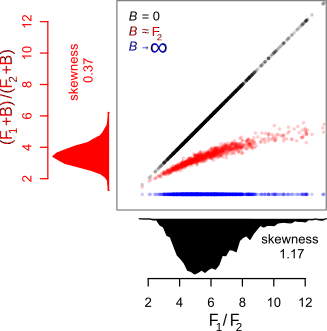
\includegraphics[width=3in]{FIGS/imaging/backgroundRatio.pdf}
  {\singlespacing 
  \caption[ Idiosyncratic effects of background on ratiometric features.]
            { Ratiometric features are idiosyncratically affected by background.
            The same initial data as in the right panels of \ar{fig:imaging:SBeffects},
			but where each single-nucleus ratio
            after addition of background is plotted against its true value (1000/3700 cells shown).
            To each average was added 0 (black), 1000 (red),
            or $10^{10}$ (blue) background units before taking the ratio. The first
            two artificial cases are the same as those in \ar{fig:imaging:SBeffects}.
			The impact on the apparent ratio
            is dependent on the relative sizes of the foregrounds and the background,
            such that the data becomes scrambled in the red curve.
            Note that
			the distribution shape is also affected, such that adding background
			decreased the skewness. $F_1$, average
            single-nuclear Hoechst; $F_2$, average nuclear Smad2/3.}
  \label{fig:imaging:backgroundRatio}}
  \end{figure}


In the second case, we could allow $F_{c1}$ and $F_{c2}$ to come
from distinct channels, which would also allow them to have
different shading
and background. As a consequence, the effects on the
distribution properties are extremely difficult to predict
due to the presence of many independent variables
(as indicated in the case study in \ar{fig:imaging:SBeffects}, right panels).
I therefore leave the discussion here, with
the conclusion that the mean and variation of the ratio feature can both
increase or decrease with different ranges of component values.
This unpredictability has important
ramifications for applications such as
fluorescence resonance energy transfer (FRET) where interpretation
relies on accurate cross-channel ratios \cite{Hodgson2010}.


\subsubsection{On the importance of image correction}

Unfortunately, the mathematical discourse above leaves us
with the dissatisfying result that the importance of image correction
is highly dataset dependent. In \ar{fig:imaging:SBeffects} I show
the size of the distortion for an example dataset with
experimentally-reasonable amounts of background and shading, which
shows effects that are measurable and sometimes relatively large. However,
different analytical requirements can tolerate quite different
amounts of feature distribution distortion before
data interpretation is affected.
The best I can do then, besides the easy blanket statement
``always correct your images!'' is to provide a few rules of thumb for
deciding on the importance of image correction.


First, I
completely ignored the detector contribution ($D$) in the above
discussion because
the matrix $D$ is unchanging and is therefore trivial to subtract from
images. Removal of $D$ should be a part of all image
analysis pipelines. This step is rarely explicitly performed
in the literature but can have a large impact
on measurements of weakly-fluorescent samples. In particular,
shading will be underestimated without subtraction of the detector
fluorescence contribution.


Second, shading tends to increase feature distribution widths
and so should be corrected whenever measurement of true biological
variability is important. Additionally, if the foreground to background ratio
is low, then shading may cause foreground values in one part of an image to fall below
background values in another part. This can have
important consequences to image segmentation \arp{imaging:segmentation}
\cite{Herbert2012}. However, in the case that biological
variability is high relative to the variation in shading
it would not be necessary to correct for $S$.
This is because the observed average and total distributions are
the convolution
of the shading and foreground distributions. If two normal distributions
with variances $\sigma^2_1$ and $\sigma^2_2$ are convolved, they yield a new
distribution with $\sigma^2_3=\sigma^2_1+\sigma^2_2$. Because shading
is a relative term, we have to scale it to the size of $F_c$ to make
use of this property: $\sigma^2_{\text{observed}}=(F_c\sigma_{S_c})^2+\sigma_{F_c}^2$.
Thus, if $F_c\sigma_{S_c}^2<<\sigma_{F_c}^2$ the observed
distribution will be close to the true distribution. While this
is a useful rule of thumb, I note that I have never observed normally-distributed
shading values (see examples in \ar{fig:imaging:properties}b).


Third, background can dramatically shift feature distribution
means. Background should therefore be corrected either when accurate means
or accurate ratios between two means are needed. When background
is low compared to even the lowest foreground values, however, it will have
little impact on the feature distributions discussed above.


Finally, when using cross-channel ratios extra care should be
taken to ensure that both background and shading are corrected.
These ratios should always be interpreted with an eye towards
the possible
effects of imaging artifacts, as artifacts can distort rations
in unpredictable ways.


\subsection{Review of image correction methods}
\label{imaging:correction:review}


Now that I have given some motivation for the importance of image correction, 
I turn to the available methods for this
process. Here, I briefly review the correction methods that
are commonly employed in the literature. In general, when deciding
on a method the investigator should test its theoretical performance
given the image model described in this chapter, $I=D+S(F+B)$.
By taking this approach, deficiencies or important assumptions of
the methods should become clear.


There are many published methods for fluorescence image correction,
perhaps as many methods as there are labs, due to the idiosyncrasies
of imaging data and the lack of standardized approaches.
I group the most common methods into two broad, non-exhaustive
categories, which I refer to as ``reference-image'' and ``per-image''
correction.
Reference-image methods obtain correction parameters from one image
and then use those parameters to correct another image. Per-image methods
find such parameters in the very image that is to be corrected.


Reference-image methods are straightforward and so are commonly used and 
recommended throughout the literature
\cite{VandenDoel1998,Model2001,Zwier2004,Wolf2007,Waters2009}.
These methods make a key assumption: that the reference image 
has approximately the same shading and background
as do the images to be corrected. A good example of this approach
uses two reference images to flatten shading, subtract background,
and normalize the fluorescence
intensity to a standard \cite{Model2001}.
One reference image, $I_\text{uniform}$ contains a
dissolved fluorophore; because this image would be flat without shading, it can
be used to determine how much shading is present in the real images. The other
reference, $I_\text{background}$ is the same as the sample images but contains no
sample. This image can thus be used to estimate background.
Equations~\ref{correction:example1}\nobreakdash-\ref{correction:example2} demonstrate this method.
	%
	\begin{align}
	I_\text{sample}     &= D+S(F_\text{sample}+B) \label{correction:example1}\\
	I_\text{background} &= D+SB \label{correction:ib} \\
	I_\text{uniform}    &= D+S(B_\text{uniform}+B) \\
	I_\text{corrected}  &= \frac{ I_\text{sample}-I_\text{background} }{ I_\text{uniform}-I_\text{background} }
		= \frac{ [D+S(F_\text{sample}+B)]-[D+SB]}{ [D+S(B_\text{uniform}+B)]-[D+SB] }
		= \frac{F_\text{sample}}{B_\text{uniform}} \label{correction:example2}
	\end{align}
	


While reference-image methods are straightforward and often easy to perform,
some of those recommended in the literature are only partially corrective. This is especially
true with respect to the detector value $D$, which
I have not seen explicitly accounted for in these methods.
To find out if a given method performed complete correction, investigators can plug the
image model into the method and check that, algebraically, the output is either
$F$ or some normalized form of it (as in \ar{correction:example2}).
However, note that partial correction may be
sufficient in some cases, particularly when background intensity is low compared
to foreground intensity and when within-image shading variation
is low compared to foreground variation.


Per-image methods, on the other hand, have the challenging task of measuring
all image components ($D$, $S$, $F$, and $B$)
within the image that is to be corrected. These methods typically
work by trying to fit a model to the combination of non-foreground
layers, $D+SB$. Therefore the primary difficulty
is that images typically contain varying fractions of foreground pixels
(e.g. due to variation in cell density),
so that determination of which pixels consist of background
is non-trivial. Further, even if identification of background pixels
is straightforward within an image, the size of the background signal
``underneath'' a foreground object is necessarily unknown and must
be predicted. The method for this prediction is what separates the different
per-image correction algorithms. 


Some per-image methods fit a polynomial \cite{L2000}
or spline surface \cite{Lindblad162266,Lindblad2004,Yin2013} to predicted
non-foreground pixels, therefore assuming a 
particular structure to the shading patterns.
These methods may also assume properties of 
the foreground objects (e.g. fluorescing cells),
such as a maximum size in the case of the rolling ball algorithm employed by
ImageJ\cite{Schneider2012} and Fiji \cite{Schindelin2012},
and may perform non-linear transformations of the underlying
images. Additionally, the accuracy of these
approaches necessarily decreases with
increasing cell density as there are fewer
background pixels from which to estimate
$I_\text{background}$. High confluency or cell clumping can thus cause
per-image methods to introduce artifacts.


When they work properly, per-image based methods generate
$I_\text{background}$ \arp{correction:ib} 
from each sample image, $I_\text{sample}$ \arp{correction:example1}.
From this point, then, the reference-based and per-image based
correction methods are the same; the only difference is in how
$I_\text{background}$ is obtained.
The question that then remains in both cases is which
mathematical operation to perform in order to correct the sample images. 
In the literature,
subtraction ($I_\text{sample}-I_\text{background}$) is frequently
used. However, subtraction does not remove
shading, as the algebraic result is $SF$ instead of $F$. The standard
rolling ball algorithm employed by ImageJ and
FIJI uses this subtractive approach.


The better approach is to use division to remove shading. This can be
done in combination with subtraction to remove both background and shading,
as in the example above \arp{correction:example2}. However, many studies
use simple division ($I_\text{sample}/I_\text{background}$), which results
in $\frac{D+S(B+F)}{D+SB}=1+\frac{SF}{D+SB}$. This result is a
background-normalized foreground with incompletely-corrected shading.
The correction can be completed by prior subtraction of $D$ from both images,
followed by subtraction of 1, which would yield the normalized image $F/B$.


I use a different approach from those listed above, 
which is to independently estimate all
non-foreground parameters so that I can perform the image algebra
that expicitly returns $F$. I discuss this method next.


\subsection{An improved correction method for high-throughput imaging}
\label{imaging:correction:myMethod}


Having determined the importance of image correction, and observed
the diversity and frequent inaccuracy of the available correction methods,
I sought to develop a simple and robust method for my own imaging applications.
All of the work in this dissertation took advantage of the throughput of
microtiter plates (e.g. 96- and 384-well plates), and so in particular I needed
to be able to accurately correct large numbers of images with
minimal computational overhead.
Further, I needed the correction to be robust to cell density,
so that I could correctly measure single-cell biological variability
under a wide variety of experimental conditions.


The approach that I developed (published in \cite{Coster2014}),
is a reference-based
method that relies on a key observation: shading patterns
are highly predictable
in microtiter plates. This allows for a correction method
that forgoes the need to
estimate parameters for every image, yet is more accurate
than using only
a single set of correction parameters. Below I show the
evidence that shading is indeed predictable, and then outline
a correction method for taking advantage of this fact.


\subsubsection{The shading pattern is a function of within-well position}



  \begin{figure}[!bt]
  \centering
  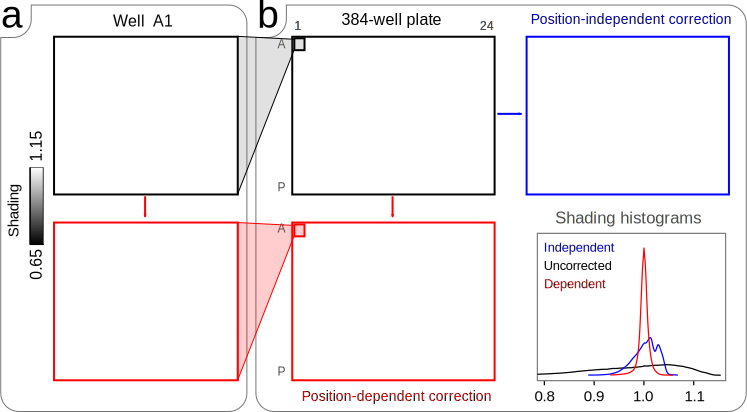
\includegraphics[width=6in]{FIGS/imaging/plateCorrection.pdf}
  {\singlespacing 
  \caption[ Demonstration of within-well positional image correction.]
            { For a within-well position, shading patterns are consistent
			throughout the entirety of a microtiter plate.
			I imaged 3x3 grids within every well of a 384-well
			plate containing dissolved fluorescein. Optical setup:
			black plastic 384-well plate (Corning \#3712), FITC filter,
			20X objective, Andor sCMOS camera.
			I cropped all images identically to remove pixels that contained
            well edges. Within-well images were montaged
			into a single image, and then normalized to the median pixel
			value of that montaged image (e.g. in \b{a}, top). This converts
			the images to an estimate of shading as defined in this chapter.
			Reference 3x3 image montages were
            made by taking the per-pixel average
			across all 3x3 montages (from all wells).
            This was done either with all 9 images in
			the 3x3 grid (Position-dependent correction) or with only the
			central image from the grid repeated 9 times
            (Position-independent correction).
			Finally, the resulting grids were montaged to show the image
			properties across the entire 384-well plate (\b{b}). Panel
			\b{a} shows larger thumbnails of the 3x3 image grids in well A1
			before and after position-dependent correction. The histograms
			in \b{b} shows the distributions of all relative pixel intensities
			in the montaged images. Tighter distributions indicate more
			accurate correction. White objects in the montaged images are
			auto-fluorescing debris; small black corners in remaining in
			corrected images are due to inclusion of a small portion
			of the black well edge.}
  \label{fig:imaging:plateCorrection}}
  \end{figure}


I was initially surprised at the high variability in shading patterns that I
observed within imaging datasets from microtiter plates.
In the literature there
appears to be an implicit assumption that such
variability is common and unpredictable,
as the most common correction methods used in big datasets are
per-image. However, shading is an artifact that is
generated by the light path, which is a static aspect of the microscope
optical setup, and so I would have expected it to be
unchanging within a dataset. Indeed, images taken at different positions along a
glass slide seem to show an unchanging shading pattern.
I therefore reasoned that it was the microtiter plates
themselves that modified the
shading pattern. Further, since microtiter plates are essentially
arrays of identical wells, I
predicted that the shading modification must be a function of the
image location
within a single well (as opposed to the position within the plate).
The source of the within-well shading modulation could be due to
reflections from well edges, local distortions
of the imaging surface, or lensing by
the solvent meniscus.


This prediction of within-well positional dependence of
shading patterns bore out, as can be seen in
\ar{fig:imaging:plateCorrection}. Further, this turned out
to be consistent for both 384- and 96-well plates from various
manufacturers and with different physical specifications
and materials. In 96-well plates
this positional effect is less dramatic, which is consistent with
shading patterns being modified by well edges (as these edges
are much further apart than are those in 384-well plates). I also note that
a position-independent correction method (that uses a single reference
image instead of one per within-well position,
\ar{fig:imaging:plateCorrection}, blue) dramatically improves
the images as well. Therefore this even simpler method may be suitable
for some datasets (though the resulting multi-modality in
\ar{fig:imaging:plateCorrection} could, in principle, generate
artificial cellular subpopulations \arp{introduction:variability}).




\subsubsection{Pipeline for within-well position-based image correction}
\label{correction:pipeline}

The within-well positional shading constancy allowed
me to implement a simple and robust image correction pipeline
for images from microtiter plates. This pipeline is based on the
existing reference-based approaches discussed above and in other
sources \cite{Bray2012,Bray2013}.




  \begin{figure}[!bt]
  \centering
  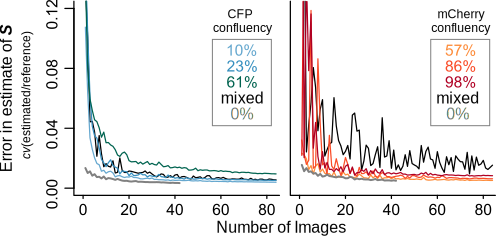
\includegraphics[width=5in]{FIGS/imaging/samplenum.pdf}
  {\singlespacing 
  \caption[ Estimating $S$ from sample-containing images.]
            { Shading ($S$) can be estimated using sample-containing
             images. Media-only wells are controls (0\% confluency).
             The spatially uniform fluorescence in these control wells was used
             to estimate the 
             ``reference'' shading by per-pixel averaging
             across 42 media-only control wells. I define
             ``confluency'' as the fraction of pixels in an image
             with intensities >3$\sigma$ above background.
             I used A549 cells expressing two differently-colored
             fluorescent proteins (left, nuclear CFP; right,
             cytosolic mCherry) at three different seeding
             densities (each seeding density had 84 replicates),
             effectively yielding six different confluency
             levels. I additionally created mixed-confluency
             image sets by randomly selecting across all
             confluency levels within each color channel.
             For each fixed number of images, $n$,
             selected from the same within-well position, I computed
             the ``estimated shading'' as the per-pixel median of
             $n$ randomly selected images. The error in the shading
             estimates are computed as the $cv$ of the per-pixel 
             ratio of (estimated shading)/(reference shading).
             For each confluency level, the inaccuracy of the
             sample-based shading estimate generally decrease
             with increasing numbers of images.}
  \label{fig:correction:samplenum}}
  \end{figure}

  

\begin{enumerate}

\item \textbf{Calibrate the microscope stage for the microtiter plate.}
Ideally, images should be acquired near well centers,
and relative within-well image positions should have
minimal drift between wells (e.g. images in well A1
should not be closer to the left well edge than those in H12).
It is important to be aware that this method will become
inaccurate with increasing positional drift. Also note that
microscope stage-driving software can vary in its accuracy,
and so custom solutions might be required for plates with
small wells.

\item \textbf{Measure the dark current component, $D$.}
The simplest approach is to capture images without a light
source, or with the light path diverted from the camera,
and per-pixel average the images. In practice, a small
number of images is sufficient ($n$=6-20 in my analyses).

\item \textbf{Subtract dark current, $D$, from all images in
the dataset.} The resulting images ($I-D$) are then modeled
by $S(B+F)$. This important step should be performed
regardless of the correction method subsequently
used, for the reasons explained above.
Without subtracting $D$, the estimated shading
patterns can become increasingly inaccurate with large
foreground values or small background values.

\item \textbf{Estimate shading $S$ for each distinct within-well
position.} This step is the most complicated in the pipeline
and should be performed with care. The goal is to obtain a
reference shading pattern for each within-well position.
For example, if an investigator has 9 images/well she will
need to estimate 9 shading patterns. There are at least two
possible approaches to this estimate.

\begin{itemize}

\item \textbf{Uniform reference images.} This approach
is the most robust, but is only possible if
there are extra wells that can be reserved solely for
acquiring reference images. In these extra wells, 
add dissolved fluorophore at the appropriate
concentration for the intended exposure time.
These wells should then be imaged along with the
other sample wells. In practice, I have found that a
small number (e.g. 6) of such uniform images is often
sufficient so long as the wells are free from fluorescing
debris. Across all wells $w$, for a given within-well
position $p$, the images $I_{w,p}$ should be per-pixel averaged
to obtain a reference image $\text{R}_p=\text{mean}_w (I_{w,p}-D)$.
Note that the per-pixel median or other quantile may
be more robust.

\item \textbf{Sample-based reference images.}
In high-throughput studies extra wells may be
unavailable for acquiring reference images.
In this case, the investigator can take advantage
of the large number of available sample images and otherwise
use the same method as for uniform reference images.
Because these sample images contain foreground, many
more values per coordinate are needed to get an
accurate estimate of shading. In \ar{fig:correction:samplenum}
I show how accuracy is dramatically affected by
the number of images used. The same figure suggests that
20-40 cell-containing images may often be sufficient, but this
is dependent on the cellular confluency of those images. 
\end{itemize}


The results of this step will be one reference image per
within-well position. As defined earlier, the shading values
should be centered on 1 to maintain the original intensity
range. Therefore once all reference images are collected
each image $\text{R}_p$ should be divided by the median
or mean of all reference image pixel values (with coordinates
$(r,c)$. The resulting shading patterns are described by
$S_p=\frac{\text{R}_p}{\text{mean}_{r,c,p} R_{r,c,p}}$


\item \textbf{Correct for the shading $S$ at each
within-well position.} To correct for shading,
every image $I_p$ should be per-pixel divided by
the corresponding shading pattern $S_p$ obtained in
the previous step: $\frac{I_p}{S_p}$. The resulting
images then contain only $B+F$.


\item \textbf{Subtract the background from each image.}
There are multiple approaches to this task.
The proper choice depends on the
particulars of the dataset, and so I illustrate two
cases here. In both cases, after subtracting background
we end up with the approximate foreground signal, $F$.

\begin{itemize}

\item \textbf{Global background subtraction.}
In some datasets, the background may vary little between
images. In this case, a global background value can be
estimated by averaging background pixels from a
representative image. Subtract this value from all pixels
in all images.

\item \textbf{Per-image background subtraction.}
In other datasets, there may be significant variability
in background from well to well. This could be due to errors
in staining or variation in exposure time. 
Background values can be estimated per image
by e.g. Otsu thresholding to automatically identify
background pixels \cite{Otsu1975}. Alternatively, a low
quantile pixel value can be taken as background
(the quantile choice is dependent on cell density).
Then, for each image, subtract its estimated
background value.


I note that, in the case of background
differences being due to something that would imply foreground
differences, such as due to exposure time or staining
variation, these per-image background estimates can be used
to normalize intensities between images. For example, to
normalize all images to some reference $B_{ref}$, determine the
normalization factor by taking its ratio with the per-image
background $B_{ref}/B_{sample}$. The image can then be multiplied by this
factor at every pixel, bringing it to the same intensity level
as the reference image. Care should be taken with this approach,
however, as it is not generally obvious when background variation
is predictive of foreground variation. 
\end{itemize}

\end{enumerate}

Note that this pipeline is only meant to remove shading $S$,
background $B$, and detector $D$ from images. What is left will
be all foreground layers, which may include various artifacts.
Further, the foreground values may vary for reasons independent
from imaging. For example, it is well established that assays
in microtiter plates can show batch, edge, row, and column effects.
These effects may non-biologically change the true values of $F$
and should thus be normalized after image correction
\cite{Malo2006,Dragiev2011,Dragiev2012,Carralot2012,Zhong2013}.

  
\subsection{Image correction quality control}

As with any data manipulation, the image correction
method outlined above should be checked to ensure
that no errors are introduced.
An obvious approach is to simply
visually inspect a subset of images, as in 
\ar{fig:imaging:flatfieldCheck}a,
though automated approaches are also feasible.


For background correction,
images should be checked to ensure that only the
background has been subtracted. This can be done
by examining background pixels. Since a perfect
subtraction will have set the centroid of the
background pixel distribution to zero, roughly half
of all post-correction background pixels should
be zero while the other background pixels take on small values.
Unfortunately, this task can be difficult to automate
for the same reason that errors may be introduced:
cell density may vary dramatically within a dataset,
complicating the automated identification of background pixels.


For shading correction, the likely artifacts will be
spatial. In other words, if there is over-correction
or under-correction,
this will cause certain regions of every image (and
the cells within those regions) to have systematically
higher or lower intensities than the global mean. This can be checked
in an automated way after cell segmentation by testing
for dependence of single-cell features on within-image
position (see an example of this approach in
\ar{fig:imaging:flatfieldCheck}b).



 \begin{figure}[!bt]
  \centering
  \includegraphics[width=6in]{FIGS/imaging/flatfieldCheck.pdf}
  {\singlespacing 
  \caption[ Quality control for image correction.]
            {Images can be over- or under-corrected, and
            therefore require quality control. \b{a},
            Visual inspection should reveal a flat background
            and a foreground that does not vary in a
            spatially predictable manner after correction. Histone H2B-Cyan
            Fluorescent Protein labeled A549 cells. Image
            courtesy Jungseog Kang (Altschuler \& Wu lab,
            UT Southwestern). \b{b},
            After segmentation and feature-extraction,
            single-cell features can be tested for within-image
            spatial dependence. Top left, a sample image of
            Smad2/3-stained human colonic epithelial cells,
            showing the radial metric of ``distance from image
            center.'' Plots show nuclear area and
            total nuclear Smad2/3 or Hoechst
            as a function of within-image radial position
            ($n$=1000/$\sim$20000 randomly-chosen cells).
            Intensities were median-normalized by well to prevent
            true experimental variation from affecting this
            test of positional phenotype dependence.
            Inset
            numeric value is the Pearson correlation coefficient
            for the two variables plotted. }
  \label{fig:imaging:flatfieldCheck}}
  \end{figure}

\section{On segmentation and single-cell features}
\label{imaging:features}


Once a dataset has been collected, and corrected as
in the previous section, the analysis begins. In general,
we want to obtain interesting properties of the foreground
layers in our images. In specific, it is nearly always the
foreground properties within individual cells that we care
about. ``Segmentation'' is the process of identifying
those cells (or intracellular objects)
and extracting them from the rest of the image.
Once cells have been segmented, properties of their pixel
values and spatial arrangement can be measured and stored
as sets of features.


Cellular segmentation is still an unsolved computer
vision problem \cite{Danuser2011},
in large part because experimental needs are too specific
to allow for a good general solution. There is, however,
an array of partial solutions available. These range from simple
to highly complex, and vary tremendously in their accuracy
and utility.
In this section I briefly discuss segmentation algorithms
and how one can go about choosing single-cell
features that are biologically meaningful.
My goal in part is to provide
the rationale for my own choices for the
experimental work in \ar{insulation:introduction}.


\subsection{Segmentation approaches}
\label{imaging:segmentation}

There are many approaches to cellular segmentation.
Software solutions such as CellProfiler \cite{Carpenter2006}
implement many of the most-used segmentation algorithms
so that the user can choose one appropriate to the experiment.
Unfortunately, which algorithm should be chosen is not a trivial matter.
Many of these algorithms are complex and therefore difficult
to understand and use. Further, the simpler algorithms may fail
to provide sufficiently accurate segmentation for some image properties.
As a consequence the path of least resistance is often manual segmentation
using tools such as ImageJ \cite{Schneider2012},
but this labor-intensive approach limits the resulting sample
size and may yield biased investigator-specific outcomes.


The value of automated segmentation approaches should be obvious:
they allow for the rapid and reproducible
identification of huge numbers of cells. Automated approaches are
also biased, due to the choice of parameters for the algorithm, but
the bias is systematic and does not change between images.
There are plenty of difficulties with automation, however. With
huge datasets comes the inability to perform thorough quality
control. Additonally, there may be no single set of segmentation parameters,
or even a single algorithm, that will successfully segment all
cellular phenotypes in a diverse experimental setup (e.g. a
drug screen). Automation thus requires extensive testing and
a wary mindset.


As a consequence of these issues, I strongly advocate for use of the simplest
segmentation method that is capable of answer a given
experimental question. Because so many aspects of images
can be measured, it is easy to get carried away with trying to
obtain every single piece of data that the images contain. As already noted, however,
the number of potential measurements is large;
obtaining all data from images is not only impossible, it probably
is not wise since each extracted feature should be understood at a
biological level before it is used (and, as I discuss below, biological
interpretation of features is not a trivial task).
The use of simpler methods makes the resulting segmentation more 
understandable, and so conditions that will cause the algorithm
to produce garbage are more predictable and intuitive. A few of
the more straight-forward and commonly-used methods are
threshold, watershed, and voronoi segmentation, discussed next
(these are depicted graphically in \ar{fig:imaging:segmentationMethods}).


  \begin{figure}[!bt]
  \centering
  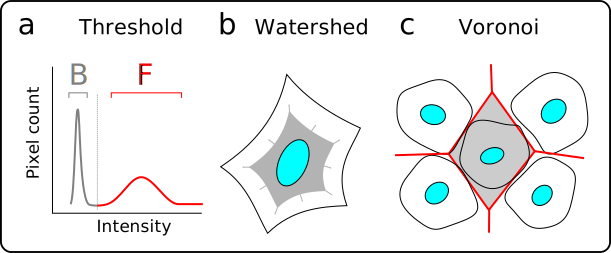
\includegraphics[width=4in]{FIGS/imaging/segmentationMethods.pdf}
  {\singlespacing 
  \caption[ Cartoon of segmentation methods.]
            {Cartoons of three basic segmentation
            methods. \b{a}, Threshold segmentation separates
            background $B$ from foreground $F$ by fluorescence
            intensity. Neighboring pixels are then considered
            part of the same object. The histogram
            represents the distribution of
            all pixel intensities within an image.
            \b{b}, Watershed starts with a known
            intracellular point (e.g. the nucleus, blue)
            and moves outwards (gray, arrows) until it reaches
            cell boundaries. \b{c} Voronoi segmentation assigns
            to a set of already-known objects all of the space closer to
            that object than any other. Red lines, boundaries
            of the Voronoi cells,
            using nuclei centroids as the known points. Gray area,
            segmented region for the middle cell.}
  \label{fig:imaging:segmentationMethods}}
  \end{figure}
  
  
Threshold segmentation (the approach that I use in this
dissertation) is probably the simplest method after manual
segmentation. It works by assuming that the pixel intensities
within cells are generally higher then those in the image
background \ar{fig:imaging:segmentationMethods}a.
Therefore a threshold can be chosen either manually
or via some mathematical or algorithmic approach (e.g.
Otsu thresholding \cite{Otsu1975}) that best separates
background and foreground pixels. Neighboring pixels classified
as foreground can be grouped into
objects, such as nuclei. This method tends to fail for whole-cell
segmentation when
cellular density is high, as neighboring cells can be segmented
as single objects. Additionally, it is not necessarily true
that the nuclear or cytosolic compartments contain higher
pixel intensities than do the background. This is dependent
on the probes used, and is of particular difficulty for
live-cell imaging (see Appendix \ar{pseg} for an experimental solution).
Cellular nuclei are frequently
segmented using this method, as they tend to be spatially distinct
even with high cell density, and DNA stains such as Hoechst
and DAPI create bright foreground signals. Threshold-segmented
nuclei often form the basis for more complex algorithms.


There are many specific algorithms for watershed segmentation
\cite{Vincent1991,Malpica1997,Loo2010} but the general
approach is roughly the same. The algorithm starts with
a ``seed,'' which is a pixel coordinate in the image.
This seed can be randomly generated or chosen from centroids
of threshold-segmented nuclei. The algorithm then searches
away from that seed point, following paths of increasing
intensity (\ar{fig:imaging:segmentationMethods}b).
Sharp decreases in intensity, as frequently
occurs between cells or between a cell edge and the background,
will cause the outward movement to stop. These algorithms
are thus useful for segmenting irregularly-shaped and slightly
crowded cytosolic regions. However, they may require many parameters, and
can yield over-segmentation (the breaking up of single cells
into many objects).


The final method that I want to make note of is Voronoi
segmentation. I have not frequently seen this method used in
the context of segmenting cells in tissue culture, but it
can be useful in the case that cells are at an extremely
high density (so that there is no background) and when
those cells are similar in size and relatively round
or cuboidal. With this approach,
a set of seeds are again needed. These will typically be
the centroids of threshold-segmented nuclei. For each centroid,
then, the algorithm assigns to it all space closer to that centroid
than to any other (\ar{fig:imaging:segmentationMethods}c).
This is a simple and efficient method for roughly segmenting
cellular cytosolic compartments.


With this brief overview of few segmentation methods, a
few points should be clear. First, many segmentation
approaches are fluorescence-based (though some use
brightfield) and so require staining of the cellular
compartments to be segmented (see Appendix \ar{pseg} for a live-cell
solution to this). Second, nuclei are much simpler
to segment than cytosolic regions, because nuclei typically
have narrower ranges of size, shape, and staining intensity.
Therefore threshold segmentation of
nuclei is generally considered to be accurate, and is
a frequent first-step for more complicated segmentation
pipelines. Third, different foreground objects may
require different algorithms for accurate segmentation.
Taken together, the above points help to explain why cellular
segmentation does not have a general solution.



\subsection{Understanding and choosing single-cell features}

Given the nearly unlimited set of features to choose from
it can be difficult to determine the subset that is most
appropriate to the study at hand. There are a few broad
approaches to this problem. The obvious, but non-trivial, approach is to
first choose the biological property of interest and then
identify or create features that approximate that property.
A less obvious approach is to obtain a large number of
features and use computational methods to choose those that
are the most informative \cite{Singh2010}.
In the latter case, the features need
not be biologically interpretable at all. For this discussion
I focus on the first case.


Biologically-motivated features are necessarily approximations
of the underlying property of interest. It is therefore important
to be aware of how the features are defined so that the data
can be interpreted properly. As an example, a project in the
Altschuler \& Wu lab required measurement of neutrophil polarity, but
needed that measurement to be performed on fluorescently-labeled
cytoskeletal components. There is no obvious mathematical
feature of fluorescently-labeled actin or microtubules that would indicate the
degree of polarization of a neutrophil. An approximate solution was
therefore developed, which measures how close together in space are the brightest
pixels \cite{Ku2010,Ku2012}.


This polarity feature will decrease in value with, for example, 
increased collection of actin to one side of the cell.
In the case that the actin intensity is diffuse throughout
the cell, the brightest pixels will also be
diffuse and so the feature value increases.
This feature therefore serves as a useful proxy for polarity. However,
the feature is sensitive to bright punctate artifacts that
are common to immunostained images and is distorted by differences in
cell size. By being aware of these pitfalls they can
be addressed. In this case, visual quality control was performed
on every cell to ensure
the absence of artifacts, and the feature calculation was modified to compensate
for distortions due to cell size \cite{Ku2010,Ku2012}.


Investigators will more frequently use combinations of
simpler features, such as those describing aspects of cell
size and shape (``morphological features'') and
of fluorescence intensity (``intensity features''). It is
important to be aware that these two classes are not completely
independennt. Intensity features in particular can be highly
dependent on morphological features.


As a simple example,
the average intensity is dependent on the area.
It is therefore important to interpret changes to the average
with care, as the change could result from  a
change in cell size, a change in concentration of the labeled
protein, or a combination of the two.
The ratio of nuclear to cytosolic average intensities
additionally suffers from this potential confusion. It has
an added difficulty, however, in that a change in the ratio
can be due to movement of the labeled protein from one compartment
to the other, or to independent changes in one or both compartments.


Ideally, then, a
feature should be carefully chosen to have an unambiguous biological
interpretation and be independent of
other features whose changes are not important to
the study. I argue that interpretability is more important than having
a feature that more closely approximates the biological property
of interest. For example, in my own work (\ar{insulation:introduction})
I am interested in the
concentrations of nuclear transcription factors. Concentration
is intuitively approximated by the average intensity feature, yet
I instead chose the total intensity feature for all of my analysis.
I did so because certain properties of the total intensity feature,
discussed next, allow for less ambiguity in how to interpret
changes in its values.


\subsection{Benefits of the total nuclear intensity feature}
\label{imaging:totalIntensity}


The total intensity
feature is a proxy for the absolute count
of a fluorescently-labeled target molecule. This feature has the
advantage of being independent of cell size, such that changes
in cell morphology may change the average but not total
intensity. Unfortunately, intensity from widefield microscopy images
does not just come from the focal plane, but also from the
space both above and below that plane. As a consequence,
in image represents a messy volumetric cross section through the $z$-axis.
This fact adds some complication to the interpretation of the
total intensity feature: is it measuring the total number of
molecules in the entire cell volume, from a thin cross-section,
or something in between?


Fortunately, my focus on transcription factors in 
\ar{insulation:introduction} allows me to mitigate this concern
by measuring only the nuclear intensities. The nucleus
tends to maintain a taller stature in the $z$-axis than does
the rest of the cell (resulting in the famous ``fried egg'' appearance
of cells in tissue culture). Also, nuclei tend to be of
more similar size and shape than do cytosolic compartments.
For these reasons, I can reasonably assume that whatever the
thickness of the imaged section, I will be imaging a similar
thickness for all nuclei.


Finally, and perhaps most importantly, the nucleus
has a built-in ``ground truth'' for this feature that allows
for both quality control and removal of measurement error
\arp{imaging:variation}.
This ground truth comes from the DNA content of cells, as
each cell within e.g. the G1 phase of the cell cycle in reality
has a near-identical total DNA content. The total intensity
feature is a proxy for this content. Importantly,
total nuclear intensity is the only feature
with such a ``ground truth'' reference.
The small-molecule stain Hoechst
provides a robust and DNA-specific signal that I use throughout
this dissertation to measure total DNA content. I therefore use
the term ``DNA'' interchangeably to refer to the actual molecule
and as a short-hand for ``Hoechst-stained DNA.'' 


\subsection{Measuring information content of a feature}
\label{imaging:information}

One of the major hurdles in experimental cell biology
is our lack of initial knowledge about which environmental
signals ($S$) and cellular responses ($R$) cells care about
(discussed in \ar{introduction:introduction}).
As a consequence, it is generally unclear how
much information about the environment a cell can accurately process
and store, though estimates suggest that the features
we believe cells care about contain
somewhat unimpressive information content \cite{Cheong2011}.

  \begin{figure}[!bt]
  \centering
  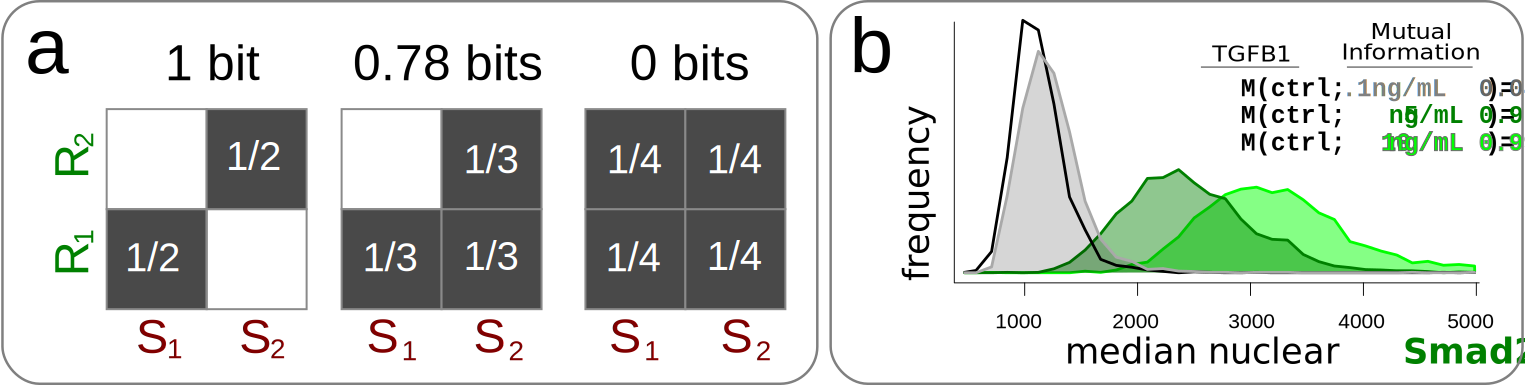
\includegraphics[width=6in]{FIGS/imaging/MI.pdf}
  {\singlespacing 
  \caption[ Mutual information examples.]
            {The mutual information metric can be interpreted
            as yielding $\log_2$ of the number of distinct signal-response
            relationships. \b{a}, A toy cases with
            only two signals, $S_1$ and $S_2$, and two responses,
            $R_1$ and $R_2$, with uniform joint probabilities. Darkened
            boxes show occurring signal-response relationships and their
            joint probabilities. Left, two completely distinct
            signal-response pairs yield $\log_2(2)=1$ bit of mutual
            information. Middle, both signals cause response $R_1$,
            meaning that observation of $R_1$ provides insufficient
            information to know which signal caused that response. The mutual
            information thus decreases to $\log_2(81/16)\approx0.78$
            bits (using \ar{eq:imaging:mi}). Right, with both signals
            causing both responses with equal probability, there is
            no mutual information ($\log_2(1)=0$ bits).
            \b{b}, Mutual information measurements of TGFB1-Smad2/3
            responses. Distributions show the wide variability
            of nuclear Smad2/3 accumulation even in response to
            saturating (10ng/mL) ligand concentrations. Observe
            that the control and saturating doses yield distributions
            that are nearly non-overlapping, and as a consequence
            yield $\sim$1 bit of mutual information (as there are 2
            distinct signal-response relatinships). It should be clear
            that the mutual information between all concentrations and
            outputs can be calculated at once, but there is significant
            overlap between all but the outermost distributions. Thus,
            addition of each subsequent intervening signal will in this
            case yield diminishing improvements to the mutual information
            between TGFB1 and nuclear Smad2/3.
            $n$>3000
            human colonic epithelial cells per condition. I used
            an implementation of the mutual information algorithm as described
            in \cite{Cheong2011}.}
  \label{fig:imaging:MI}}
  \end{figure}

Measuring the information content of a feature with
respect to the signal under study can therefore be useful
when trying to choose between a set of potential $(S,R)$
combinations. This can be
done using the ``mutual information'' metric
between the signal and response, $M(S;R)$  \cite{Cheong2011}.
Mutual information has advantages over other statistical metrics,
such as Z-scores and the like, in that it is completely
non-parametric (i.e. does not assume a distribution shape)
and uses units that
can be directly interpreted as ``information content,'' measured in bits.
I use this metric in \ar{insulation:introduction} to compare
the information content of ligand concentrations for \tgfbsf\
and Wnt, and so here I dig into mutual information a bit
deeper\footnote{Did you catch the joke?}
with the goal of providing an intuition to the reader
regarding its interpretation.


The mutual information between a set of signals $S$
(e.g. ligand concentrations) and
responses $R$ (e.g. nuclear transcription factor concentrations) is defined
by \ar{eq:imaging:mi}. In the formula, $P(R,S)$ is the joint
probability of each signal-response pair
and $P(R)$ and $P(S)$ are the marginal
probabilities.
The mutual information value returned by this formula
is in units of ``bits,'' and can
be interpreted as the $\log_2$ of the number of
distinct signal-response relationships
(see \ar{fig:imaging:MI}a for a toy example).
In essence the quantity describes how accurately
we would be able to guess the signal if we were
told the response (and vice versa).
The goal of the mutual information metric then
is to measure the degree of overlap between
signal-response distributions, it is not to measure
how far apart those distributions are. For example,
two completely separated response distributions will
always have 1 bit of mutual information even if they
are infinitely far apart. Therefore the maximum possible
information content is $\log_2$ of the number of distinct
signals (\ar{fig:imaging:MI}a, left). The minimum mutual information is zero, which
occurs when the distributions completely overlap (\ar{fig:imaging:MI}a, right).
    %
    \begin{equation} \label{eq:imaging:mi}
    M(R;S)=\sum_S\sum_R P(R,S)\log_2\left(\frac{P(R,S)}{P(R)P(S)}\right)
    \end{equation}



Importantly, single-cell
variability in nuclear transcription factor
concentrations is high, such that even the
untreated and saturating ligand
doses yield a small overlap in cellular
responses (\ar{fig:imaging:MI}b) \cite{Cheong2011}. In other words,
if we were given a randomly drawn cellular Smad2/3
response from a dose-response curve for TGFB1 treatment,
we would have high uncertainty as to the precise
TGFB1 concentration that caused the drawn response.


In summary, mutual information is a metric that
measures the overlap of distributions, and so can
be interpreted to indicate the number of distinct
signal-response pairs for a given feature. This
metric can thus be used to directly measure the
relative information content of different features $R$
or signals $S$ (as I do in \ar{insulation:system}).

\section{Dealing with variation}
\label{imaging:variation}


Experimental error is always present in our
measurements. Additionally, any given feature
may show extensive biological variability even within
apparently homogeneous populations. The biological
variation can be informative, as it gives us
insight into the limits to accuracy of cellular
processing and can reveal phenotypically distinct
subpopulations (see \ar{insulation:introduction}).
However, if experimental error is mis-interpreted
as biological variability, we lose statistical resolution
or may assign unwarranted meaning to non-biological
variation. It is then important to be able to separate
experimental from biological variation.


Experimental variation in fluorescence imaging
comes from many sources.
The imaging plane itself may cause
variation by intersecting cells at different
relative heights. This focal plane effect
can cause cell-to-cell differences in the
degree of focus and in how much off-plane
fluorescence is captured. As discussed
in \ar{imaging:distortion}, image shading and
background can also contribute to artificial variation
due to microscopy.


Aside from microscopy artifacts, the process
of preparing cells for imaging may also
generate distortions of true biological variability.
For example, variation in cellular surface
area or volume may lead to differences
in how well an antibody or non-permeable dye
can access an intracellular target.
Such differences in cell morphology may be
enhanced or dampened by fixatives, which can cause cells to shrink
in the $z$-axis \cite{Pawly2006}.


  \begin{figure}[!bt]
  \centering
  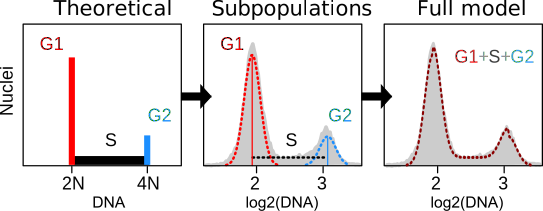
\includegraphics[width=4in]{FIGS/imaging/cycleFit.pdf}
  {\singlespacing 
  \caption[ Fitting total DNA to a simple cell cycle model.]
            {An asynchronous cell population can be
            fit to a simple model of the cell cycle
            with reasonable accuracy. Left,
            the theoretical
            asynchronous cell-cycle distribution consists
            of delta functions for G1 and G2 cells (i.e.
            all cells in these populations have identical
            DNA content) and a uniform distribution for
            S-phase cells that are moving from the G1 to G2
            states at a constant rate. Middle, the
            total DNA feature of G1 and G2 nuclei shows log-normal variation
            that can thus be fit to normal distributions after log-transformation.
            Right, the cell subpopulation models 
            add up to a reasonably accurate estimate
            of the cell cycle distribution. Gray, filled
            histograms are of $\log_2$(total DNA), with 
            DNA in arbitrary units, of $\sim2\times10^4$ Hoechst-stained
            human colonic epithelial cells. Dashed lines are
            the actual fits to this data using the method described
            in the text.}
  \label{fig:imaging:cycleFit}}
  \end{figure}


Finally, non-biological variation can be introduced
during segmentation. This can be due to outright errors
(e.g. a cell being split into two objects) or to
the more subtle fact that the accuracy of a set of
segmentation parameters will vary from cell to cell.
For example, a chosen threshold that perfectly separates
background from foreground for one cell may end up
discarding the outer edges of a dimmer cell.


\subsection{Using DNA features for quality control}
\label{imaging:variation:dnaQC}

Due to the error sources discussed above (among others)
there may be many outlier cells to discard. Manual or pseudo-manual
approaches are often used for this task. 
Visual inspection of a random
subset of segmented cells is a common approach,
though automated solutions are needed for large datasets.
An example is the identification of out-of-focus images using
image-level features from tools like PhenoRipper
\cite{Rajaram2012}.
I use an automated statistical approach that takes
advantage of ``ground truth'' aspects of total DNA
content in cells. 
This approach uses population-level statistics
of DNA features to determine which cells
are likely to be properly
segmented and in focus. In effect, I make the assumption that
cells with biologically-unlikely DNA feature values will have
non-biological values in other features as well.




  \begin{figure}[!bt]
  \centering
  \includegraphics[width=6in]{FIGS/imaging/qualityControl.pdf}
  {\singlespacing 
  \caption[ Using DNA features for quality control.]
            {DNA features can be used for single-cell quality
            control. Bottom left, the Total DNA feature
            is fit to a cell cycle plot (fit not shown)
            and the G1 population is gated as all cells
            within $\mu_{G1}\pm2\sigma_{G1}$ (blue). The population is
            also statistically gated using the nuclear area (bottom,
            middle) and the intra-nuclear intensity $cv$ (bottom, right).
            The gating is $\pm3\times\text{MAD}$ from the median of each
            feature, where $\text{MAD}$ is the median absolute deviation
            ($\text{median}(|X-\text{median}(X)|)$. 
            ($3\times\text{MAD}\approx2\sigma$ for normal distributions.)
            The gated points are considered to be in-focus G1 cells
            that are likely segmented properly. In the top plot,
            these quality-controlled
            cells are found as red points within the blue box. Data from
            >4000 Hoechst-stained human colonic epithelial cells.}
  \label{fig:imaging:qualityControl}}
  \end{figure}



The first step in my quality control pipeline is to identify cell cycle
subpopulations by fitting a cell cycle model
to the total DNA histograms. This allows for later isolation
of these subpopulations and removal of outliers. Note that
in tissue culture microscopy
mitotic (M-phase) cells are often lost during sample washes
and so are already excluded from analysis.


An asynchronous cell population can be accurately
fit to a simple model of the cell cycle. The
theoretical, variation-free model of this cell cycle
consists of of delta functions for the G1 and G2 peaks
with a uniform S-phase distribution in between
(\ar{fig:imaging:cycleFit}, left). In other words, all
cells within G1 or G2 have the exact same DNA content,
and cells moving through S-phase increase their DNA content
at a constant rate. In reality,
the cell cycle distribution arising from measured
total DNA consists of $\log$-normally distributed G1
and G2 peaks, with a variable-shaped S-phase distribution
in between. I note that, on a $\log$-scale, the G1 and
G2 distributions have near-identical standard deviations
($\sigma_{G1}\approx\sigma_{G2}$).



I implemented a simple variant of the
Dean-Jett-Fox cell cycle model \cite{Dean1974,Fox1980}
that is sufficient to accurately identify G1 and G2 cells
from microscopy data.
The formulae that comprise this model are in
Equations~\ref{eq:imaging:g1}\nobreakdash-\ref{eq:imaging:g2},
where: $T_c$ is the $\log_2$-transformed
total DNA of a single cell; $\mu_{G1}$ is the average of this
value across all G1-phase cells; $\sigma$ is the standard
deviation of the G1 and G2 distributions; $v$ is the height of the S-phase
uniform distribution, $f(T_c)$ is the fraction of
cells with the same $T_c$ DNA content (in practice, it is the fraction of cells
falling into the same histogram bin), and $w$ values are weights. \ar{fig:imaging:cycleFit} shows
this model graphically, fit to experimental data.
    %
    \begin{align}
    f_{G1}(T_c) &= \frac{w_1}{\sigma \sqrt{2\pi}}
    e^{-\frac{(T_c-\mu_{G1})^2}{2\sigma^2}} \label{eq:imaging:g1}\\
    f_{S} (T_c) &= \left\{
        \begin{array}{lr}
        0 & : T_c \notin [ \mu_{G1}, \mu_{G2} ] \\
        v & : T_c \in    [ \mu_{G1}, \mu_{G2} ]
        \end{array}
        \right.
    \label{eq:imaging:s}\\
    f_{G2}(T_c) &= \frac{w_2}{\sigma \sqrt{2\pi}}
    e^{-\frac{(T_c-\mu_{G2})^2}{2\sigma^2}} \label{eq:imaging:g2}
    \end{align}


While fitting to a cell cycle distribution model may
be sufficient to identify biological outlier cells, I use two
additional DNA features to further exclude low-quality
images of nuclei. These features
are the nuclear area and the coefficient of variation ($cv$)
of intra-nuclear DNA intensity.
The $cv$ is a rough proxy for the DNA texture,
and so can be used to identify out-of-focus cells
(lower $cv$) or those with chromatin condensation or
punctate artifacts (higher $cv$). I therefore statistically
gate the population by rejecting those cells that are too
far from the median of either of these features
(see \ar{fig:imaging:qualityControl}).


Finally, I restrict my analyses to cells in the G1 phase
\arp{fig:imaging:qualityControl}.
The rationale for this is that I do not expect G1
and G2 cells to have different qualitative behaviors
for the signaling pathways that I study in \ar{insulation:introduction},
though I do expect them to have somewhat different quantitative
behaviors. The effect of combining these subpopulations
would then be a meaningless increase in apparent signaling variability.
I therefore chose the G1 population as it is
typically more populated and is less prone to
double-segmentation errors.


\subsection{Using DNA features to correct measurement error}


By using DNA features for quality control, we can thus collect
all cells within the G1 and/or G2 populations that are high-quality
(from an imaging standpoint) and accurately segmented.
The quality control described above may be a sufficient level of
data clean-up for some experimental goals, but
it does not deal with the problem
identified at the top of this section: 
that is, the separation of true biological variation from
measurement error. In other words, quality control only discards
cells that are too far from the ``typical'' cell, it does nothing
to determine or correct the measurement error in those cells that are kept.


To identify biological variability, then,
I again take advantage of the cell cycle ``ground truth.''
As shown in \ar{fig:imaging:cycleFit}, the theoretical
cell cycle distribution has no variation in the G1 or G2
populations, as all cells have exactly the same diploid
or tetraploid DNA content. The observed variation
around the theoretical values then do not carry any biological
meaning. (Note that this approximation becomes less accurate
with chromosomally-unstable cell populations.)


\subsubsection{Single-cell measurement error correction}
\label{imaging:singleCellCorrection}

If the variation in total DNA carries no biological
information, then it should not be predictive of
of other feature values: any feature dependence on
the DNA content must then be due to a global source
of error. In principle, then, we can then reduce this error by 
removing the meaningless correlations of other features to total DNA content. 


  \begin{figure}[!bt]
  \centering
  
\includegraphics[width=6in]{FIGS/imaging/singleCellNorm.pdf}
  {\singlespacing 
  \caption[ Single-cell correction using DNA features.]
            {The variation in total DNA content (within a single cell cycle peak)
            is non-biological and therefore should not be predictive of
            intensity values for other probes.
            \b{a}, Total Smad as a function of
            total DNA. The raw data show a low
            Pearson correlation coefficient (inset $r$ value)
            and linear regression slope (black line),
            which is over-corrected by
            multiplicative normalization (middle) and
            corrected by regression-based normalization
            (right). \b{b}, Comparison of single-cell values
            before (x-axis) and after (y-axis) regresson-based
            correction. This dataset has low correlation to
            total DNA, and so the change is small. 
            $n=689$ human colonic epithelial cells (G1 only,
            quality-controlled) immunostained
            with anti-Smad2/3 (Smad) and Hoechst (DNA).
            All $y$-axes on the same scale.}
  \label{fig:imaging:singleCellNorm}}
  \end{figure}

I take two single-cell level approaches to correcting
total intensity feature errors
\arp{fig:imaging:singleCellNorm}. The intuitive method
is to estimate a normalization factor for e.g. all G1 cells
using total DNA ($T_{\text{DNA},c}$), and then use this
factor to normalize the total intensity of other
fluorescent probes ($T_{\text{probe},c}$)
in those same cells (\ar{eq:imaging:dnaNorm}). Indeed,
I have seen this approach used in the literature even
without first restricting analysis to one cell cycle
subpopulation. This
method assumes a simple multiplicative relationship
between the DNA and other channels such that, for example, a 10\%
increase in total DNA content would predict a 10\%
increase in different total probe intensity. Note
that this assumption may not hold true, such that this
method can cause over- or under-correction (as in
\ref{fig:imaging:singleCellNorm}a, middle).
    %
    \begin{equation} \label{eq:imaging:dnaNorm}
    f_{\text{norm}}(T_{\text{probe},c})=
    \frac{\text{median}_c(T_{\text{DNA},c})}{T_{\text{DNA},c}}T_{\text{probe},c}
    \end{equation}

    
My preferred method is regression-based, as it
guarantees removal of
correlation between total Hoechst and the total intensity of
another probe (\ar{fig:imaging:singleCellNorm}a, right).
For this method, linear regression is performed to get the
function in \ar{eq:imaging:reg} with slope $m$ and intercept $b$.
This results in a residual value ($\text{r}_{\text{probe},c}$)
for every cell.
The value of each $T_{\text{probe},c}$ can then be corrected
by setting it equal to the median across all values plus the residual
value for the same cell (\ar{eq:imaging:regNorm}).
    %
    \begin{gather}
    T_{\text{probe},c}=f_\text{regression}(T_{\text{DNA},c})=mT_{\text{DNA},c}+\text{r}_{\text{probe},c}+b
        \label{eq:imaging:reg}\\
    f_\text{norm}(T_{\text{probe},c}) =
        \text{median}_c(T_{\text{probe},c})+\text{r}_{\text{probe},c}
        \label{eq:imaging:regNorm}
    \end{gather}

    
For the sample data in \ar{fig:imaging:singleCellNorm} it is
clear that there is low basal correlation between total DNA
and total Smad, though I have observed much
higher correlations in some datasets. I further note that this same rationale
could be extended to non-DNA references and other features
for cases in which cross-probe
correlations are expected to be meaningless.
For all datasets in this dissertation I
apply the total DNA regression-based correction when accurate
single-cell values are needed (such as for the calculation of mutual
information between single-cell distributions).


\subsubsection{Population-level error correction}


While the single-cell correction above can be used to remove
those measurement errors that are directly shared by each probe,
it is reasonable to expect that much
of measurement error is more random and so affects probes independently. Though it is
not possible to correct single-cell values for such
unpredictable error, we can apply correction at the
population level.


  \begin{figure}[!bt]
  \centering
  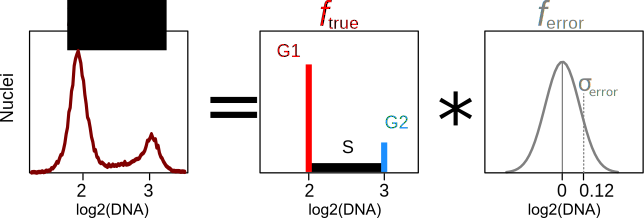
\includegraphics[width=4in]{FIGS/imaging/convolution.pdf}
  {\singlespacing 
  \caption[ Estimating measurement error of the total intensity feature.]
            {An observed total intensity distribution $f_\text{observed}$
            is the result of convolution of the true distribution
            $f_\text{true}$ and the measurement error $f_\text{error}$.
            The error function for total nuclear intensity features
            can be estimated as having $\sigma_\text{error}\approx
            \sigma_\text{DNA}$.
            Cartoon, using distributions from \ar{fig:imaging:cycleFit}.}
  \label{fig:imaging:convolution}}
  \end{figure}


An observed feature distribution can be modeled as the convolution
of a true biological distribution with a measurement error
distribution centered on zero, $f_{true}*f_{error}$. In the case of $\log$-total DNA
in G1 cells, $f_{true}$
is a delta distribution, $\delta_{true}$, positioned at $\mu_{G1}$.
I can then take advantage of
the property that $\delta_{true}*f_{error}=f_{error}+\mu_{G1}$.
In other words, the G1 and G2 distributions are themselves
estimates of the measurement error distribution, if their
means are set to 0
\arp{fig:imaging:convolution}.


For distributions that are log-normal, as are the total
intensity features for all probes used in this dissertation,
I can also use the property that two convolved normal distributions
yield a third normal distribution with mean
$\mu_3=\mu_1+\mu_2$ and variance
$\sigma_3^2=\sigma_1^2+\sigma_2^2$.
Thus, I can estimate the ``true'' cell-to-cell
total nuclear intensity variation
for any probe by \ar{eq:imaging:decon}. There of course may
be other sources of error not compensated for in this way, and
such an approach is only defensible for the total intensity feature.
    %
    \begin{equation} \label{eq:imaging:decon}
    \sigma_\text{probe,true} = \sqrt{ \sigma_\text{probe,observed}^2-\sigma_\text{DNA,error}^2 }
    \end{equation}

    
What utility does this deconvolution have? Published
measurements of cell-to-cell
variability range from 15-30\% \cite{Sigal2006a},
and my own raw data show values within
this same range. However, these values include measurement error
that is not being compensated for. Thus,
cell-to-cell variability, as measured by microscopy, is
necessarily overestimated. The above reasoning shows that
this overestimation is simple to measure, as all that is
needed are the log-scale standard deviations of the G1/2
total DNA distributions and the standard deviations of
the total-probe values in question.


I have not performed a comprehensive
study of the size of this effect, though I have measured it
in several independent datasets for various markers. I find
that deconvolved total intensity distributions yield
$\sim10\%$ lower standard deviations and $\sim10\%$ higher
information content (measured by mutual information \cite{Cheong2011}).
These inaccuracies are small enough that I feel comfortable
stating that measurement errors in high-quality microscopy datasets
are much smaller
than true biological variation.


It is important to note
that this DNA-based deconvolution makes the assumption
that the sources of error are the same between Hoechst and other probes. It is
possible that nuclear antibody-based stains have a partially non-overlapping
set of error sources with small molecules like Hoechst.
One possibility to address this, then, would be to use a
non-specific secondary antibody in a free channel.
That non-specific antibody should
not be correlated with the specific antibody staining in other
channels, and so any measured correlations could be removed using the
same rationale as for DNA content-based correction. Unfortunately,
I have had limited success with this
approach, though non-specific secondary antibodies
do indeed show high single-cell correlation. The problem has been that they also
show unexpected properties, like differences in intracellular
localization, for which adequate controls are not clear.



\section{Discussion}
\label{imaging:discussion}

Unlike other quantitative single-cell
methods, such as flow cytometry, the subcellular resolution of
image data allows for a stupefyingly
large number of feature measurements, and there are no standardized
practices for choosing or implementing these
features. Further, identification of individual
cells takes place at the level of software, not
hardware. Quantitative imaging is thus an
exceedingly difficult task outside of the labs
that specialize in it, and no two of these labs
are likely to converge on the exact same solutions.


With imaging we can directly see the beauty of the
biology we are studying, and the high information
content of images makes this type of data boundless
in its potential utility. We are currently not
meeting this potential, however, and I firmly believe
that this is due to an absence of established standards
and approaches that would make quantitative imaging more broadly accessible
and interpretable. To that end, I hope that this chapter
provides some intuition to those scientists who have
not had the opportunity to work and think extensively
about image data. Further, I hope that my approach
to single-cell image analysis, described in this chapter
and demonstrated in \ar{insulation:introduction} for
a specific biological study, provide useful demonstrations of the utility
of quantitative single-cell analysis.




\section{Methods}
\label{imaging:methods}

This chapter provides the imaging and image analysis details
also
used for the experiments in \ar{insulation:introduction}.
The methods for cell culture, immunostaining,
and imaging are left to that chapter (see \ar{insulation:methods}).
Specific methodological details for the figures in
this chapter are primarily provided within the figure
legends; this section provides the remaining information.


\textbf{Cell culture.} I followed the methods in
\ar{insulation:methods}, with the following additions.
For \ar{fig:correction:samplenum}, I used a fluorescently-labeled
clone of the cell line A549 (ATCC \#CCL-185). This clone
contains a pSeg vector that co-expresses
Cyan Fluorescent Protein fused to
Drosophila Histone H2B to label nuclei and the
Red Fluorescent Protein variant mCherry to label the whole cell
(see Appendix \ar{pseg}). The clone was generated by
Jungseog Kang and Qi Wu (Altschuler \& Wu lab, UT Southwestern).


\textbf{Imaging.} Plates were imaged on one
of two Nikon Eclipse Ti-E2000 microscopes controlled by NIS
Elements version 4, using several optical setups. Image coordinates
were generated using NIS Elements or custom software for higher
precision. The cameras used were either a Roper Scientific CoolSnap
HQ2 CCD 14-bit \ar{fig:imaging:SBeffects} or an Andor Zyla sCMOS 11-bit.




\chapter{Conclusion}
\label{conclusion:introduction}


The study of cellular signaling is a difficult one, in large
part because we know so little, \i{a priori}, about what aspects
of a signal a cell cares about and into what intracellular properties
it encodes those signals. It may be, however, that the complexity of
our understanding of signaling is hiding a reality of underlying simplicity
(\ar{introduction:introduction}). In particular, the static
network models that we rely on include links derived from
different timescales (such that activity along one link
should be considered constant relative to activity along another)
as well as links that may only be present in a
subset of true signaling network instances
(e.g. in certain cell types or experimental conditions).


Wnt/\bcat\ and \tgfbsf\ together
provide a case study for this problem of signaling
complexity (\ar{pathways:introduction}).
For each pathway alone there is a lack
of clarity due to idiosyncratic outcomes between
labs and experiments. There is even less
clarity when considering how the two pathways are integrated
by cells in order for them to make decisions.
Much of the confusion
regarding crosstalk between these pathways may stem
from the reliance of published work on overexpression assays,
which can push cells into abnormal states. Further,
the same studies rely on transcription-based
readouts that are measured long after initial pathway 
activation, allowing for transcriptional feedback to confound
the results \arp{pathways:discussion}. 


Therefore, I tested Wnt/\bcat\
and \tgfbsf\ for crosstalk using an assay that relies on
endogenous levels of proteins (to prevent the signaling networks
from being pushed into abnormal states), short timecourses
(to prevent transcriptional feedback from confounding 
interpretation), and direct readouts of signal transduction
\arp{insulation:introduction}.
This study design allowed me to directly test the affect
of signaling through one pathway on signaling through the other.
In this way, I discovered that Wnt/\bcat\ and \tgfbsf\ are in fact
completely insulated from one another during signal transduction.
Further, I found no evidence for the expected intra-\tgfbsf\ inhibition
nor the competition for the shared component, Smad4, thought to cause it.


Though I observed that signaling insulation is a general
phenomenon, I did uncover an instance of context-dependent
transcriptional crosstalk. Importantly, the resulting transcriptional
feedback led to biasing of signaling
activity over longer timecourses. In effect, this is a direct
example of the fact that some network links may exist only under certain
conditions, and that experimental separation of signaling and transcription is essential
to understanding the nature of morphogenic pathway integration.
From these results, I conclude that there exists a surprising simplicity
of interactions between morphogenic pathways: there is a high degree
of insulation between Wnt/\bcat\ and \tgfbsf, allowing nuclei to make
transcriptional decisions based on more-complete models of their environments
(\ar{insulation:discussion}).


For the experimental approach that led to my discoveries,
I relied heavily on quantitative, single-cell fluorescence
microscopy (\ar{imaging:introduction}).
Single-cell imaging is an increasingly available
and invaluable approach
to studying cell biology (and cell signaling in particular).
Unfortunately, single-cell image analysis is a difficult and unsolved problem.
An oft-neglected issue is that of image correction, prior to
analysis. Indeed, the most commonly-used methods throughout the literature
tend to provide incomplete or error-prone image correction.
I discovered a solution to this problem, in the particular case
of high-throughput microscopy, which takes advantage of predictable optical
properties within microtiter plates (\ar{imaging:correction}).


\subsubsection{On negative results}


When I first found that Wnt3A and \tgf 3 are insulated
from one another during signaling, I was hugely disappointed. This disappointment
came, in large part, from having spent a year under the impression
that there actually was crosstalk. I had performed many experiments
and narrowed down the point of inter-pathway crosstalk to the receptor
or ligand level, before I finally discovered contamination of the purified
recombinant Wnt3A ligand (\ar{fig:insulation:contamination}).


The artifactual result itself was not the most disappointing part;
it was instead the feeling that I now had a ``negative result'' and would
therefore have to drop the project completely and start over.
This attitude had been ingrained within me throughout my science
education: I was taught that scientific discovery is about finding
new and exciting things. Or, in any event, that my discoveries would need to be
new and exciting in order to get published and move my career forward.


While scrambling to make the best out of the situation, I slowly
realized that there was not truly a problem. The fact that the crosstalk
I observed was an artifact was a real result: numerous studies
show signaling interactions between these pathways, and the contaminated
reagent is among the most commonly used for studying Wnt/\bcat\
signaling. As long as I
could unambiguously demonstrate the absence of crosstalk, then my result
was not a negative one at all and could potentially reduce some confusion
in the field. One person's negative result is another person's positive
result, as it were.


In any case, there is value to negative results. In recent years there
has been increasing hubbub in the news and in opinion pieces regarding
the state of biomedical research. Of particular concern has been the
irreproducibility of published results and the toxic effects of
using ``impact'' as the primary metric for determining the merit
of both scientific discoveries and of the scientists who make those discoveries
\cite{Schatz2014,Alberts2014}. Why does the emphasis on impact lead to
irreproducibility? 
A needed statistic when evaluating a claim
is the \i{a priori} likelihood of that claim being true;
when the literature is biased towards exciting (i.e. unlikely)
results because scientists do not publish ``negative'' results, 
we cannot accurately
estimate the likelihood of truth for new claims. This problem
is (in)famously addressed in a paper by John Ioannidis
that should be required reading for all biologists \cite{Ioannidis2005}.


\subsubsection{Parting thoughts}


The overarching field of cellular signaling is an exciting one;
understanding how cells communicate and process information
is absolutely fundamental to our understanding of all of
cell biology. Importantly, a deep understanding of this
topic will allow us to more ably manipulate biological systems,
both in medicine and in bioengineering.
To develop that deep understanding, however, it is essential
that we revisit the complex static maps of established cellular signaling
pathways, and then pay careful attention to how time and context
reshape these networks. By identifying underlying simplicity
in cell signaling, we will be better equipped to both understand
and control cellular information processing and decision-making.


% BACKMATTER
% Appendices


\glsaddall



\begin{appendices}

\chapter[The pSeg plasmid library]{pSeg: plasmids for live-cell segmentation}
\label{pseg}

This dissertation uses only fixed-cell microscopy
assays, but future studies would ideally include
live-cell studies of \tgfbsf\ and Wnt signaling.
Live-imaging and fixed-cell imaging can use the same
general analytical methods,
including the use of nuclear and cytosolic fluorescence
to identify these two cellular compartments. However,
finding appropriate labels for live-cell assays is much more difficult,
as the cells are not permeabilized and toxic stains must
be avoided. In order to effectively deploy segmentation
algorithms, the nucleus and cytosol should ideally be labeled
brightly and homogeneously.


 \begin{figure}[!b]
  \centering
  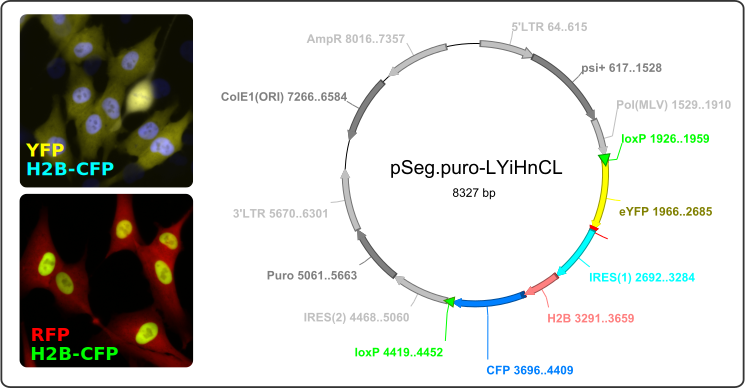
\includegraphics[width=6in]{FIGS/pseg/structure.pdf}
  {\singlespacing 
  \caption[ pSeg structure and sample images.]
            { The pSeg plasmids generally consist of two
            differentially-localized fluorophores. Left, sample
            images from two human colonic
            epithelial cell (HCEC) pSeg clones. The top image is from
            the LYiHnCL pSeg construct shown at right,
            and the bottom image is from an LRiHnCL construct.
            See \ar{table:pseg:symbols} for symbols.
            Right, structure of pSeg construct. The 5' and
            3' Murine Leukemia Virus LTRs
            (long terminal repeats) flank the
            construct, which also has loxP sites oriented
            in the same direction so that the construct
            can be excised by Cre recombinase, thus reverting
            a clone to a ``parental'' phenotype. AmpR, ampicillin
            resistance gene. psi+, viral packaging sequences. Puro,
            puromycin. IRES, internal ribosome entry site.}
  \label{fig:pseg:structure}}
  \end{figure}

One approach to address this problem is via ``central dogma'' (CD)
tagging, in which a fluorescent-protein-encoding gene surrounded by
splice acceptor/donor sites is randomly integrated
into the genome. Any integration that lands within an intron of a gene
has a chance to become an exon for that same gene. Thus,the genetic protein
product will then contain a fluorescent protein as one of its domains,
allowing the localization and dynamics of that protein to be visualized
\cite{Jarvik1996,Jarvik2002}.


High-throughput studies have used this technique to obtain
nucleus- or cytosol-localized labels for the purpose of segmentation,
with the purported benefit that it requires no exogenous expression system
and thus minimizes perturbations to the cell
\cite{Sigal2006,Sigal2007,Sigal2006a,Issaeva2010}. Unfortunately,
the CD-tagging process is slow, since exon-generating integration
events are rare and must be subsequently screened to identify
the rarer-still events that yield the desired localization patterns.
Additionally, the tagging of a protein is itself a perturbation that
may disrupt localization or function. Chosen CD-tagged clones must
then be carefully studied to ensure that the cells (and the tagged
proteins) behave properly.


A much faster alternative is to express
fluorescent proteins from exogenous promoters, though there is
always the concern that the presence of an exogenous promoter may
affect the cell in some unpredictable way. To me, this
is just as problematic as the concern that CD-tagging will
disrupt some unknown function of the tagged protein.
I therefore prefer the efficiency of the exogenous approach.
To take advantage of this efficiency for future live-cell projects, I
created a library of viral constructs, each generating distinct
localization patterns of red, yellow, and cyan fluorescent
protein expression in mammalian cells. I refer to these
as ``segmentation plasmids'' (pSegs).


    \begin{table}[!bt]
    \centering
	\footnotesize
    \caption[List symbols for the pSeg library.]
    { List symbols for the pSeg library in \ar{table:pseg:library}.}
    \label{table:pseg:symbols}
    \begin{tabular}{cll}
    \hline
    Symbol   & Abbreviation & Full \\ \hline
    C & CFP  & mCerulean\\
    G & GFP  & enhanced Green Fluorescent Protein\\
    H & H2B  & Histone H2B (\fly)\\
    i & IRES & Internal ribosome entry site (encephalomyocarditis virus)\\
    L & loxP & loxP site \\
    n & NLS  & Nuclear Localization Signal (SV40)\\
    m &      & membrane- localized Gap43 N-terminus (\i{Danio rerio})\\
    R & RFP  & mCherry\\
    Y & YFP  & enhanced Yellow Fluorescent Protein\\
    \hline
    \end{tabular}
    \end{table}



\subsubsection{pSeg structure}


Each pSeg plasmid has three variable components:
a fluorescent protein (FP) with a whole-cell expression
pattern, a fluorescent protein with a nuclear
expression pattern, and a selection cassette.
I chose the mCherry, eYFP, and Cerulean fluorescent proteins
because they have wide spectral separation and so can all
be used simultaneously in single cells.
The general structure of the insert is
shown in \ar{fig:pseg:structure}.
Whole-cell expression patterns are generated by either
free FP or a FP fused to the Gap43 membrane localization
signal \cite{Livet2007}.
This signal results in faint whole-cell and strong
membrane fluorescence.
Nuclear expression is mediated by addition of either a
nuclear localization sequence (NLS) or fusion to \fly\ histone H2B.
The H2B-fused FP is useful because it can be used to
monitor chromatin condensation \cite{Snippert2011} and
seems to be benign even when generally expressed in mice
\cite{Neurohr2009}.

   \begin{table}[!bt]
    \centering
	\footnotesize
    \caption[List of pSeg plasmids.]
    { Full list of plasmids in the pSeg library. See
     \ar{table:pseg:symbols} for symbol meanings. ``Floxed''
     refers to flanking by loxP.
     PuroR and NeoR refer to puromycin or neomycin resistance
     cassettes.}
    \label{table:pseg:library}
    \begin{tabular}{lll}
    \hline
    floxed \& PuroR & floxed \& NeoR & NeoR   \\ \hline
    LmYiHnCL        & LYiHnCL        & YiHnC  \\
    LmCiHnCL        & LGiHnCL        & YiHnY  \\
    LmRiHnCL        & LRiHnCL        & CiHnC  \\
    LmYiCnnCL       & LYiCnnCL       & CiHnY  \\
    LmCiCnnCL       & LGiCnnCL       & YiCnnC \\
    LmRiCnnCL       & LRiCnnCL       & YiYnnY \\
    LYiHnCL         &                & CiCnnC \\
    LGiHnCL         &                &        \\
    LRiHnCL         &                &        \\
    LYiCnnCL        &                &        \\
    LGiCnnCL        &                &        \\
    LRiCnnCL        &                &        \\ \hline
    \end{tabular}
    \end{table}


Each construct is expressed as a single
mRNA, using the retroviral promoter and an internal
ribosome entry site (IRES) for differential translation
of the the protein products. Finally, the constructs are
also flanked by loxP sites and so can be removed after
genomic integration, thus generating unlabeled ``parental'' cell lines.
The pSeg library consists of 25 color/localization/selection 
combinations in Puromycin or Neomycin-resistant backgrounds,
with or without flanking loxP sites.
\ar{table:pseg:library} shows all of
these constructs (refer to \ar{table:pseg:symbols} for symbol definitions).


I built the library into
the pMYs retroviral backbone, which contains a modified
version of the Murine Leukemia Virus promoter that
improves integration efficiency in some stem cell systems \cite{Kitamura2003}.
The pMYs backbone contains the viral long terminal repeats
(LTRs) and a viral packaging signal (\ar{table:pseg:symbols}), allowing for the creation
of virus using MLV packaging cell lines. 


\subsubsection{Generating cellular pSeg clones}


Integration of the pSeg constructs into target
cells requires the generation of and infection by
live virus (see \nameref{pseg:methods}). A few days
after infection, I FACS (Flow-assisted cell sorting)-sort
single cells into each well of 384-well
plates. I find that survival rates
for singly sorted cells are quite low ($\sim$20-30\%), though
I could double these rates by pre-seeding the
wells with un-labeled cells. The feeder cells can
be selected against later according to the chosen pSeg cassette.
With this appraoch, a clone from the A549 cell line was created in the
Altschuler \& Wu lab by Jungseog Kang and Qi Wu, which
forms the foundation of a CD-tagged library (unpublished).


The slowest part of the process is the establishment of clonal
cell lines from single cells, which can take 6 weeks.
However, this step is essential.
Cell-to-cell variability can be high, even within
a clonal population \cite{Singh2010}. Further, I found that all
pSegs yield populations with diverse localization patterns.
For example, the LRiHnCL construct should express
mCherry and Cerulean in the nucleus, and yet all
possible patterns are observed (\ar{fig:pseg:mixed}).
The reason for this is not clear, though retroviruses
(such as MLV) have diploid genomes within viral
particles and are known to have recombination events
\cite{Coffin1997}. The high degree of repetition within
these constructs (the different fluorescent proteins
have high homology) may then lead to truncations or
expansions of the integrated sequence, such that it
re-arranges the localization signals on the fluorescent
proteins.


Finally, I warn that the Murine Leukemia Virus has
a strong preference for integration into the 5' end
of highly-expressed genes
\cite{Wu2003a,Mitchell2004,Cattoglio2010}. Despite this
preference, the virus does seem to
avoid house-keeping genes, though I note that this
may simply be due to the death of cells that do have
integrations at such sites. As a consequence of integration,
then, functionally important genes may be disrupted. A simple test for
this is to select multiple labeled clones and compete each
against the unlabeled parental population. The clones with the
most similar-to-parental growth rates can then be kept for further experiments. 


 \begin{figure}[tb]
  \centering
  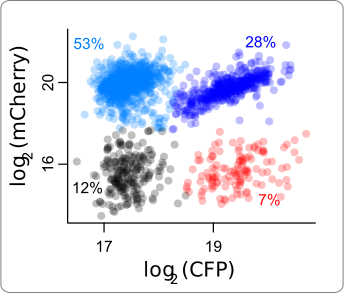
\includegraphics[width=3in]{FIGS/pseg/mixed.pdf}
  {\singlespacing 
  \caption[ Requirement for pSeg clonal selection.]
            { A population of cells infected with the
              pSeg.puro-LRiHnCL construct show all possible
              nuclear localization patterns. Percents show
              the relative population size for each group.
              The bottom-left (black) cells are unlabeled,
              the top-right (dark blue) cells are correctly
              labeled with both fluorescent proteins, and
              the other two populations express only one
              of the two proteins. $n$=1770 human colonic
              epithelial cells, stained with Hoechst for
              segmentation. Arbitrary total fluorescence units.}
  \label{fig:pseg:mixed}}
  \end{figure}






\subsubsection{Methods}
\label{pseg:methods}

\b{Molecular cloning.}
I constructed the pSeg library using a combination 
of standard moleculuar cloning techniques and 
Gibson assembly (New England Biolabs \#E5510)
\cite{Gibson2010}. I verified each construct
by Sanger sequencing, and confirmed each phenotype
by checking the localization patterns in 
transiently-transfected HEK293T cells.


\b{Tissue culture.}
The tissue culture methods and imaging followed those
in \ar{insulation:methods} with the exception of
viral production and infection.
I used the Platinum-A HEK293T packaging
cell line (Cell Biolabs \#RV-102)
and closely followed the protocol used by Uri Alon's
group for CD-tagging \cite{Sigal2007}. 
In brief, virus is generated by transfecting packaging
cells and collecting the supernatant 2-3 days later. This
supernatant is then applied to the target cells, which
are left for 48-72 hours to allow for genomic integration. The
multi-day timeline is essential, as MLV can only
integrate into immediately-post-mitotic
genomes \cite{Roe1993}.


\b{Analysis.}
For the analysis in \ar{fig:pseg:mixed} I used the ImageJ
implementation of the rolling ball algorithm for
correction and a custom Matlab nuclear threshold segmentation algorithm.
I used the Hoechst channel
to manually gate the G1 population and to subsequently
correct the mCherry and Cerulean channels using the
regression method described in
\ar{imaging:singleCellCorrection}. I used
the k-means algorithm implemented in R to automatically
identify each of the subpopulations shown in the figure.




\end{appendices}


%\glossarystyle{listhypergroup}
\footnotesize{
\printglossary[style=mcolindex,title=Glossary]
}


% Bibliography

	\singlespacing
	\small{
	\renewcommand{\chapter}[2]{}
	\clearpage
	\begin{multicols}{2}
	\bibliographystyle{ieeetr}
	\bibliography{REFS/library}
	\end{multicols}
	}

\end{document}





%% FIGURE TEMPLATE
%\begin{figure}[ht!]
%\centering
%\includegraphics[width=6in]{FIGS/figure.pdf}
%{\singlespacing 
%\caption{ The caption.}
%\label{fig:figure ref}}
%\end{figure}
